\documentclass[final]{fhnwreport}       %[mode] = draft or final
                                        %{class} = fhnwreport, article, 
                                        %          report, book, beamer, standalone
%%---Main Packages-----------------------------------------------------------------------
\usepackage[english, ngerman]{babel}	%Mul­tilin­gual sup­port for LaTeX
\usepackage[T1]{fontenc}				%Stan­dard pack­age for se­lect­ing font en­cod­ings
\usepackage[utf8]{inputenc}				%Ac­cept dif­fer­ent in­put en­cod­ings
\usepackage{lmodern}                    %The newer Font-Set
\usepackage{textcomp}					%LaTeX sup­port for the Text Com­pan­ion fonts
\usepackage{graphicx} 					%En­hanced sup­port for graph­ics
\usepackage{float}						%Im­proved in­ter­face for float­ing ob­jects
\usepackage{ifdraft}                    %Let you check if the doc is in draft mode

%%---Useful Packages---------------------------------------------------------------------
\usepackage[pdftex,dvipsnames,table]{xcolor}  %Driver-in­de­pen­dent color ex­ten­sions for LaTeX
\usepackage{csquotes}                   %Simpler quoting with \enquote{}
\usepackage{siunitx} 					%A com­pre­hen­sive (SI) units pack­age
\usepackage{listings}					%Type­set source code list­ings us­ing LaTeX
\usepackage[bottom]{footmisc}			%A range of foot­note op­tions
\usepackage{footnote}					%Im­prove on LaTeX's foot­note han­dling
\usepackage{verbatim}					%Reim­ple­men­ta­tion of and ex­ten­sions to LaTeX ver­ba­tim
\usepackage[textsize=footnotesize]{todonotes} %Mark­ing things to do in a LaTeX doc­u­ment
\usepackage{booktabs}
\usepackage{lscape}
\usepackage{blindtext}
\usepackage{wrapfig}
\usepackage{caption}
\usepackage{romannum}

%%---Tikz Packages-----------------------------------------------------------------------
\usepackage{standalone}
\usepackage{tikz}
\usepackage{circuitikz}
\usetikzlibrary{arrows}
\usetikzlibrary{calc}
\usetikzlibrary{intersections}

%%---Math Packages-----------------------------------------------------------------------
\usepackage{amsmath}					%AMS math­e­mat­i­cal fa­cil­i­ties for LaTeX
%\usepackage{amssymb}					%Type­set­ting symbols (AMS style)
%\usepackage{array}						%Ex­tend­ing the ar­ray and tab­u­lar en­vi­ron­ments
%\usepackage{amsthm}					%Type­set­ting the­o­rems (AMS style)

%%---Table Packages----------------------------------------------------------------------
\usepackage{tabularx}					%Tab­u­lars with ad­justable-width columns
%\usepackage{longtable}
\usepackage{multirow}					%Create tab­u­lar cells span­ning mul­ti­ple rows
\usepackage{multicol}					%In­ter­mix sin­gle and mul­ti­ple columns

%%---PDF / Figure Packages---------------------------------------------------------------
\usepackage{pdfpages}					%In­clude PDF doc­u­ments in LaTeX
\usepackage{pdflscape}					%Make land­scape pages dis­play as land­scape
\usepackage{subfig}					    %Fig­ures di­vided into sub­fig­ures

%%---Other Packages----------------------------------------------------------------------
%\usepackage{xargs}                     %De­fine com­mands with many op­tional ar­gu­ments

%%---Bibliography------------------------------------------------------------------------
\usepackage[style=ieee,urldate=comp,backend=biber]{biblatex}
\addbibresource{literature/bibliography.bib}

%%---Main Settings-----------------------------------------------------------------------
\graphicspath{{./graphics/}}			%Defines the graphicspath
%\geometry{twoside=false}				    %twoside=false disables the "bookstyle"
\setlength{\marginparwidth}{2cm}
\overfullrule=5em						%Creates a black rule if text goes over the margins => debugging


%%---User Definitions--------------------------------------------------------------------
%%Tabel-Definitions: (requires \usepackage{tabularx})
\newcolumntype{L}[1]{>{\raggedright\arraybackslash}p{#1}}    %column-width and alignment
\newcolumntype{C}[1]{>{\centering\arraybackslash}p{#1}}
\newcolumntype{R}[1]{>{\raggedleft\arraybackslash}p{#1}}

%%---Optional Package Settings-----------------------------------------------------------
%Listings-Settings: (requires \usepackage{listings}) => Example with Matlab Code
\lstset{language=Matlab,%
    basicstyle=\footnotesize\ttfamily,
    breaklines=false,%
    morekeywords={switch, case, otherwise},
    keywordstyle=\color{Blue},%
    tabsize=2,
    %morekeywords=[2]{1}, keywordstyle=[2]{\color{black}},
    identifierstyle=\color{Black},%
    stringstyle=\color{Purple},
    commentstyle=\color{Green},%
    showstringspaces=false,%without this there will be a symbol in the places where there is a space
    numbers=left,%
    numberstyle={\tiny \color{black}},% size of the numbers
    numbersep=9pt, % this defines how far the numbers are from the text
    %emph=[1]{word1, word2,...},emphstyle=[1]\color{red}
}					

			                %loads all packages, definitions and settings	

									
\title{\Huge{\textbf{Wetterstation mit Solar Energie}}\\}          %Project Title
\author{\huge{Bachelor Diplomarbeit 2019}}          %Document Type => Technical Report, ...
\date{Brugg/Windisch, \today}             %Place and Date
%%%%%%%%richtigerTeil%%%%%%%
\begin{document}

%%---TITLEPAGE---------------------------------------------------------------------------
\selectlanguage{ngerman}                %ngerman or english
\maketitle
%\vspace*{-1cm}
\vspace*{-0.5cm}						    %compensates the space after the date line.
\vfill
\begin{figure}[H]
\centering
%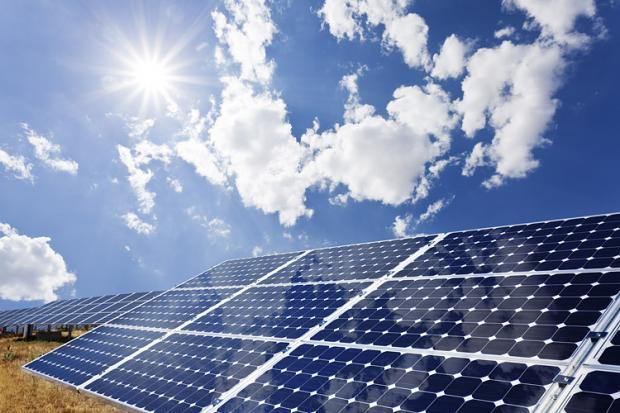
\includegraphics[width=\linewidth]{Titelbild.jpg}
\end{figure}
\vfill

{
\renewcommand\arraystretch{2}
\begin{center}
\begin{tabular}{p{4cm} l}
\textbf{Hochschule}				&	Hochschule für Technik - FHNW\\
\textbf{Studiengang}			&	Elektro- und Informationstechnik\\
\textbf{Autoren}				&	Mischa Knupfer, Andres Minder\\
\textbf{Auftraggeber}			&	Prof. Dr. Taoufik Nouri\\
\textbf{Experte}				&	Patrick Strittmatter\\
\textbf{Betreuer}				&	Prof. Dr. Taoufik Nouri\\
\textbf{Version}				&	2.1 %Normally not used!
\end{tabular}
\end{center}
}

\clearpage
			
%%---ABSTRACT----------------------------------------------------------------------------
\selectlanguage{english}				%ngerman or english
%\thispagestyle{empty}
\pagenumbering{Roman}
\begin{abstract}
\noindent
Climate and weather data are the main sources to determine plots for specific plants or plant species for a specific climate. Because of that, farmers need to know the climate and weather data to optimize their work. Swiss farmers have the advantage of getting this information through a federal agency, which does not apply to farmers in subtropical areas. To provide these information for farmers in subtropical areas, a low-priced mobile weather station is required. This project should design a prototype of a weather station, which can record data for air temperature, Rainfall, wind strength and hours of sunshine. In addition to that, the DS3231 real time clock (RTC) should generate a timestamp to the data before it is stored in the data memory. The core of the weather station is the microcontroller ArduinoMega2560, which contains the program code and manages the data storage. The wind strength is being measured by the WD123 from Froggit, the rainfall by an ombrometer from Misol and the air temperature by the BME280 from Bosch that measures also humidity and pressure of the air. Moreover, a wind vane (p/n 80422) from Argent Data Systems allows the weather station to determine the wind direction. Those gained data points are stored on an internal microSD card.\\[0.5cm]
The mobile weather station is able to provide data for temperature, humidity and pressure of the air as well as the Rainfall and the strength and direction of the wind. Furthermore, the mobile weather station is also able to store the data points with timestamp on the microSD card. In a further project, a battery will be implemented which will be supported by photovoltaic. Furthermore, GPS and data query over SMS (GSM) will also be implemented in that further project.\\
\\
Key Words: mobile weather station, sensors, microSD card, GPS, SMS (GSM)


\end{abstract}	

%%---TABLE OF CONTENTS-------------------------------------------------------------------
\selectlanguage{ngerman}				%ngerman or english
\tableofcontents
\clearpage

%%---TEXT--------------------------------------------------------------------------------
\pagenumbering{arabic}

\cleardoublepage
\thispagestyle{empty}
\vspace*{4cm}
\begin{center}
	\section{Einleitung}
	\label{sec:EinleitenderTeil}
\end{center}
\newpage
\subsection{Einleitung}
\label{subsec:einleitung}
Pflanzen benötigen eine ihnen entsprechende Umwelt. Durch meteorologische Messdaten kann diese ermittelt und durch Agronome optimal bewirtschaftet werden. Ausserdem können bei genügend Messdaten aus einem Erfassungsnetz Wetterprognosen erstellt werden. Die Erhebung solcher Messdaten trägt somit erheblich zum wirtschaftlichen Erfolg in der Agronomie bei und kann bei einem geeignet grossen Erfassungsnetz Bewohner vor Unwetter warnen. In den ärmeren Teilen Afrikas und Südamerikas sind solche Systeme jedoch nicht verbreitet. Aus diesem Grund wird eine kostengünstige, erweiterbare und mobile Wetterstation realisiert, welche die örtlichen Agronomen unterstützen kann. Diese Wetterstation kann die Niederschlagsmenge, die Windstärke \& -richtung, die Lufttemperatur, -druck, -feuchtigkeit und die Sonnenstunden messen. Außerdem kann der Akkumulator der Wetterstation mittels Photovoltaik geladen werden. Die erhobenen Daten sind via SMS\footnote{Mittels GSM/GPRS-Modul} abrufbar und mit einem GPS-Modul kann der Standort der mobilen Wetterstation erfasst werden. Zusätzlich kann mittels eines Terminals (z.B. PuTTY) eine Verbindung über eine serielle Schnittstelle über den USB 2.0 micro-B Anschluss der Wetterstation erstellt und mit ihr kommuniziert werden.\\

Mittels Ombrometer mit Kipplöffelprinzip wird die Niederschlagsmenge ermittelt. Die Windstärke wird über ein Schalenkreuzanemometer und die Windrichtung über einen Windrichtungsgeber eruiert. Über einen RJ-11 Stecker werden diese dann an die Wetterstation angeschlossen und die analogen Signale von einer Mikrocontrollereinheit ausgewertet. Die Lufttemperatur, -druck und -feuchtigkeit werden über den digitalen Kombinationssensor BME280 von \textit{Bosch} und die Beleuchtungsstärke (Lux) zur Ermittlung der Sonnenstunden über den Light-To-Digital Converter TSL2561 von \textit{TAOS}\footnote{Texas Advanced Optoelectronic Solutions} gemessen. Um den Messdaten einen Zeitstempel beifügen zu können, wird die Extremely Accurate Real Time Clock DS3231 von \textit{Maxim Integrated} verwendet. Diese drei digitalen Elemente sind über das I$^{2}$C-Interface mit der Mikrocontrollereinheit verbunden. Zur Datenspeicherung wird eine $\mu$SDHC-Karte verwendet. Im Kommunikationsmodul SIM808 von \textit{SIM Com} werden das GSM/GPRS- und GPS-Modul vereint.\\

Die (Teil-)Realisierung\footnote{Es wird in weiterführenden Projekten weiter daran gearbeitet} dieser Wetterstation wurde in zwei Projekten an der Hochschule für Technik der FHNW im Studiengang Elektro- und Informationstechnik durchgeführt. Diese bestehen aus einem vorangehenden Projekt 5, sowie dem anschließenden Projekt 6 (Bachelor Diplomarbeit) und wurden vom gleichen Team bearbeitet. Dieser Bericht umfasst die Inhalte beider Projekte. Welche Aspekte in welchem Projekt behandelt wurden, können dem Kapitel \ref{subsec:Ziele} \nameref{subsec:Ziele} direkt entnommen werden.\\

\todo[inline]{Berichtaufbau}

\subsection{Auftragsbeschreibung}
\label{subsec:Auftrag}
Das Wetter spielt eine wichtige Rolle in der Agronomie. Regnet es nicht genug, müssen Pflanzen bewässert werden. Trifft auf ein Ort nur wenig Sonnenlicht, so sollten dort nicht die Pflanzen, welche viel Sonnenlicht brauchen, angebaut werden. Windet es zu stark, können Pflanzen beschädigt oder gar zerstört werden. Ist es Tagsüber heiss, so benötigen die Pflanzen mehr Wasser. Hiesige Bauern besitzen den Luxus von guten Wettervorhersagen dank dem Bundesamt für Meteorologie und Klimatologie (MeteoSchweiz). Dieser Luxus ist in anderen Ländern noch nicht gegeben. Prof. Dr. Nouri Taoufik ist aufgefallen, dass in subtropischen Gegenden wie teile Südamerikas oder Afrikas dieser Luxus ebenso fehlt. \\

Aus diesem Grund soll eine kostengünstige, erweiterbare und mobile Wetterstation entwickelt werden, welche diese Bauern unterstützt. Diese Wetterstation soll die Regenmenge, die Windstärke, die Lufttemperatur und die Sonnenstunden messen können. Ausserdem soll die Wetterstation mittels Photovoltaik unterstützt werden, und erhobene Daten via SMS abrufbar sein. \\

Die detaillierte Aufgabenbeschreibung ist im Anhang \ref{appendix:Lastenheft} \nameref{appendix:Lastenheft} und Anhang \ref{appendix:aufgabenstellung} \nameref{appendix:aufgabenstellung} aufgeführt.\\

\include{sections/einleitung/ziele}
\subsection{Konzept}
\label{subsec:Konzept}
\begin{figure}[h]
	\centering
	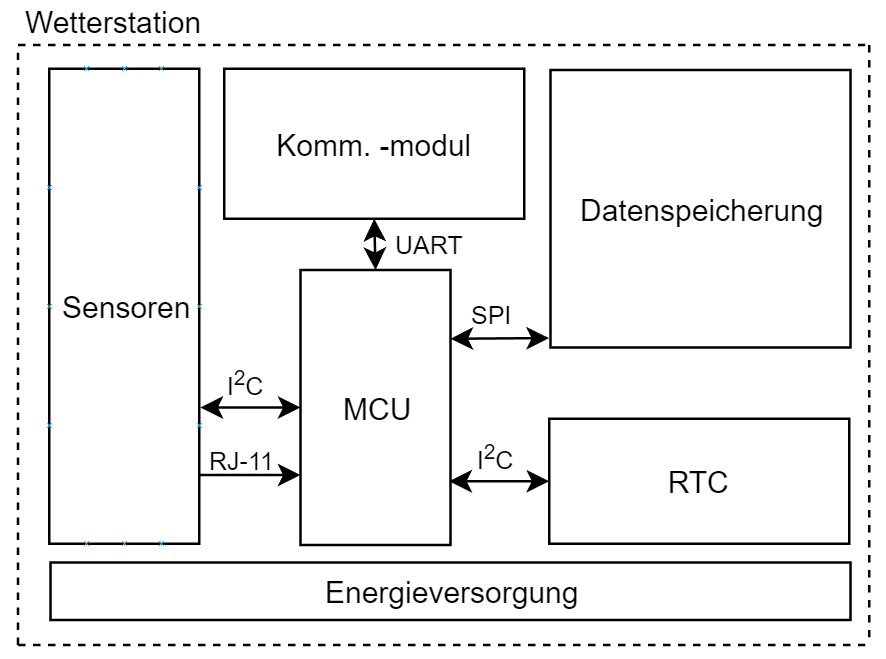
\includegraphics[width=0.9\textwidth]{graphics/Konzeptdiagramme/Grundkonzept.PNG}	
	\caption{Konzeptionelle Übersicht}
	\label{fig:grundkonzept}
\end{figure}

Das Gesamtkonzept ist, wie in der Abbildung \ref{fig:grundkonzept} grafisch dargestellt, modular aufgebaut. Die gestrichelte Linie beschreibt die Systemgrenze der Wetterstation. Als Zentralrecheneinheit wird eine \textit{Micro-Controller-Unit (MCU)} verwendet. Diese ist dafür verantwortlich, dass die Daten richtig verarbeitet und an die entsprechenden Module weitergeleitet werden. Die Messdaten werden in digitaler Form über das I$^{2}$C-Interface vom Modul \textit{Sensoren} an die \textit{MCU} übertragen. Über die RJ-11 Anschlüsse werden analoge Signale übermittelt. Dieser fügt mit dem \textit{Real-Time-Clock (RTC)} einen Timestamp hinzu, wobei anschließend die Daten in der \textit{Datenspeicherung} nichtflüchtig gespeichert werden. Über das \textit{Kommunikationsmodul} können dann die Daten von Nutznießern abgefragt werden.\\

\newpage

\subsubsection{Sensoren}
In dem Block \textit{Sensoren} (Abbildung \ref{fig:sensoren}) sind alle Messeinheiten untergebracht. Die Idee dieses Blockes besteht darin, dass dieser adaptiv ist und somit leicht erweitert werden kann.\\

\begin{figure}[h]
	\centering
	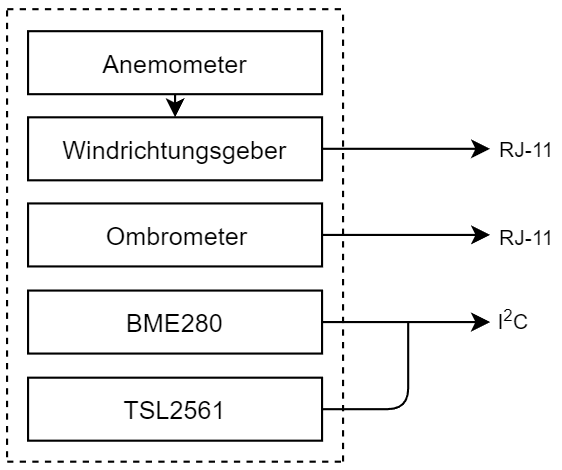
\includegraphics[width=0.5\textwidth]{graphics/Konzeptdiagramme/Sensoren.PNG} 
	\caption{Sensoren}
	\label{fig:sensoren}
\end{figure}

Der Lufttemperatur, -druck und -feuchtigkeits kombinierte Sensor BME280 und der Light-To-Digital Converter TSL2561 sind beide über das I$^2$C-Interface mit der \textit{MCU} verbunden. Das Anemometer kann direkt mit dem Windrichtungsgeber über die vorhandene RJ-11 Buchse angeschlossen werden, wobei dann der Ausgang des Windrichtungsgebers beide analogen Signale überträgt. Das Ombrometer wird separat angeschlossen.\\

\subsubsection{RTC}
Die Extremely Accurate Real Time Clock DS3231 (RTC) wird nur zur Zeitabfrage für einen Timestamp verwendet. An die \textit{MCU} ist sie über das I$^{2}$C-Interface angeschlossen. In der Abbildung \ref{fig:rtc} ist noch ein zusätzlicher Block \textit{CR2032} zu erkennen, der eine Knopfbatterie beschreibt. Sie hat den alleinigen Zweck, dass wenn mal keine Boardspeisung mehr vorhanden und somit der Akkumulator der Wetterstation leer ist, das RTC noch immer Speisung hat. Das RTC läuft dann weiter und muss bei einem kurzzeitigen Ausfall nicht gleich zurückgesetzt werden.\\

\begin{figure}[h]
	\centering
	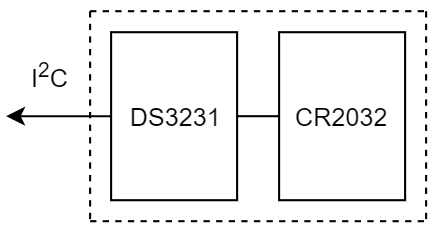
\includegraphics[scale=0.6]{graphics/Konzeptdiagramme/rtc.PNG}
	\caption{Real-Time-Clock (RTC)}
	\label{fig:rtc}
\end{figure}


\subsubsection{Datenspeicherung}
Die nichtflüchtige Datenspeicherung erfolgt auf einer $\mu$SD-Karte. Dabei werden die Wetterdaten pro 10 Minuten einmal in einem *.txt File gespeichert. Zu den gespeicherten Daten zählen:
\begin{itemize}
	\item Lufttemperatur, -druck, feuchtigkeit
	\item Windgeschwindigkeit, -stärke
	\item Regenmenge
	\item Bestrahlungsstärke
	\item GPS-Koordinaten
	\item Speicherzeitpunkt
\end{itemize}
Der Vorteil bei der Speicherung auf einer $\mu$SD-Karte ist, dass bei einem Komplettausfall der Wetterstation die Daten trotzdem problemlos mittels entfernen der $\mu$SD-Karte extrahiert werden können.\\

\subsubsection{Kommunikationsmodul}
Abbildung \ref{fig:kommunikationsmodul} zeigt die verschiedenen Schnittstellen, über welche Daten mit der Umgebung (User) und \textit{MCU} ausgetauscht werden können.\\

\begin{figure}[h]
	\centering
	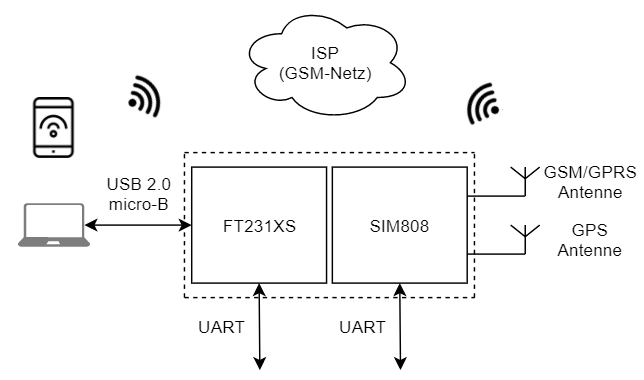
\includegraphics[scale=0.7]{graphics/Konzeptdiagramme/Kommunikationsmodul.PNG}
	\caption{Kommunikationsmodul}
	\label{fig:kommunikationsmodul}
\end{figure}

Der User hat die Möglichkeit, per Computer die Daten der Wetterstation direkt abzufragen, oder aber auch über sein Mobilfunktelefon mittels SMS. Dafür benötigt der User eine zusätzliche SIM-Karte vom lokalen Internet Service Provider\footnote{Z.B. Swisscom, Salt, Sunrise, usw.} (ISP) für die Wetterstation, welche er dann mittels Computer über die serielle Schnittstelle entsperren kann.\\

\newpage
\subsubsection{Energieversorgung}
\label{subsubsec:energieversorgung}

In der Abbildung \ref{fig:Energieversorgung} ist die Systemgrenze (gestrichelte Linie) der mobilen Wetterstation ersichtlich. Innerhalb dieser Systemgrenze befinden sich der \textit{Akkumulator}, der \textit{MCP73871} Ladechip, der \textit{LM1117} 3.3V Linearregler und der \textit{LMC7660} Spannungswandler. Ausserhalb der Systemgrenze sind die Photovoltaikanlage, rsp. das Solarpanel, das 230V AC-Stromnetz und ein Computer. Das Solarpanel, sowie auch das Stromnetz können über einen DC Jack Stecker mit den Dimensionen 5.5mm Aussen- und 2.1mm Innendurchmesser angeschlossen werden. Zusätzlich ist der Akkumulator ebenfalls über den USB 2.0 micro-B Anschluss mittels Computer ladbar. Somit kann die Wetterstation auch bei ungenügender Sonneneinstrahlung geladen werden. Es ist möglich, beide Anschlüsse gleichzeitig angeschlossen zu haben.\\

\begin{figure}[h]
	\centering
	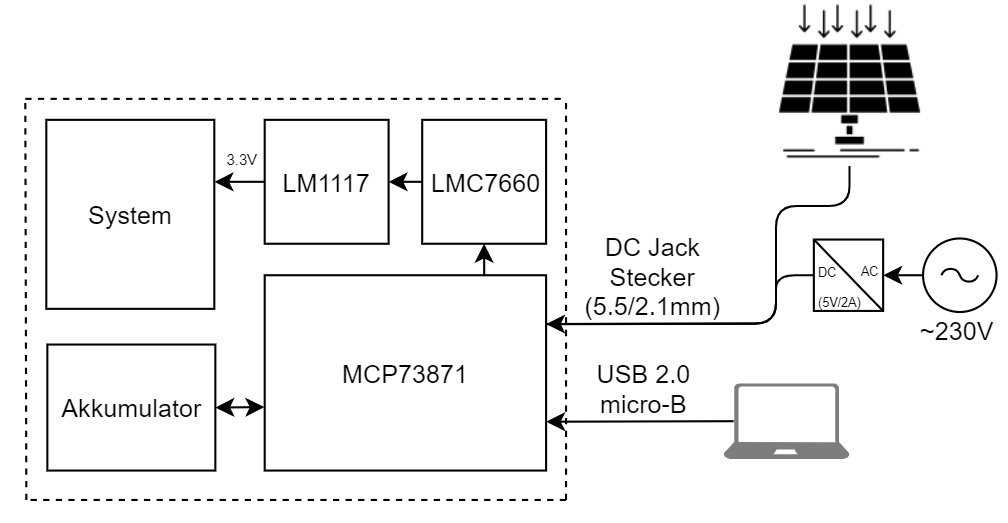
\includegraphics[scale=0.5]{graphics/Konzeptdiagramme/Energieversorgung.PNG}
	\caption{Energieversorgung}
	\label{fig:Energieversorgung}
\end{figure}

Der \textit{Akkumulator} bildet das Kernstück der Energieversorgung, da dieser die Quelle für die mobile Wetterstation ist. Er dient als Stützung der Versorgungsspannung (3.3V), falls die Wetterstation nur über das Solarpanel betrieben wird, damit sie auch in der Nacht funktionstüchtig bleibt. Der \textit{MCP73871} ist der Ladechip. Dieser reguliert den Ladestrom in Abhängigkeit des Laststromes vom System. Damit der \textit{LM1117} konstant 3.3V als Systemspannung generieren kann, wird der \textit{LMC7660} als positiver Spannungsmultiplizierer vorgeschaltet. Der Funktionsblock \textit{System} beinhaltet alle Bauteile der Wetterstation, welche mit 3.3V Versorgungsspannung betrieben werden müssen. Da die Wetterstation auf Low Consumption ausgelegt wird, sind dies fast alle Bauelemente.\\
 


\cleardoublepage
\thispagestyle{empty}
\vspace*{4cm}
\begin{center}
	\section{Firmware}
	\label{sec:Firmware}
\end{center}
\newpage
\subsection{Development Environment}
\label{subsec:dev_envir}
Die Firmware der Wetterstation wurde im AtmelStudio 7 der Atmel Corp. und der Arduino IDE geschrieben. Die Arduino IDE wurde hauptsächlich verwendet, um notwendige Librarys über dessen \textit{Library Manager} hinzuzufügen. Dies war besonders für die Sensoren BME280 und TSL2561, sowie für die RTC DS3231 und das Schreiben/Lesen der $\mu$SD-Karte notwendig. Anschliessend konnte das gesamte Projekt ins AtmelStudio importiert werden. Grund für diese Importierung ist, dass über AtmelStudio ein ISP (In-System-Programmer) verwendet werden kann. Dies ist mit der Arduino IDE nicht möglich. Der Vorteil bei der Verwendung eines ISP's liegt darin, dass der Mikrocontroller auch nach dem Einbetten in die Hardware programmierbar bleibt. Das Programm wurde in der C/C++ Syntax objektorientiert geschrieben und aufgebaut, somit ist die Firmware der Wetterstation skalierbarer und übersichtlicher.\\

Zur Übersicht der verwendeten Toolchain dient die Tabelle \ref{tab:toolchain}. Zusätzlich sind auch die Downloadlinks der aktuellen Versionen darin enthalten. Die gesamte Toolchain ist als Freeware erhältlich.\\

\begin{table}[h]
\renewcommand{\arraystretch}{1.5}
\centering
\caption{Toolchain}
\label{tab:toolchain}
\begin{tabular}{llp{8cm}}
\toprule 
\textbf{Programm} & \textbf{Version} & \textbf{Link} \\ 
\toprule 
AtmelStudio 7 & 7.0.1645 & \url{https://www.microchip.com/mplab/avr-support/atmel-studio-7} \\ 
\hline 
Arduino IDE & 1.8.5 & \url{https://www.arduino.cc/en/main/software} \\ 
\hline 
PuTTY & 0.71 & \url{https://www.putty.org/} \\ 
\bottomrule 
\end{tabular} 
\end{table}

\subsubsection{In-System-Programmer}
\label{subsubsec:insystemprogrammer}

\begin{minipage}[b][6.5cm][t]{0.5\textwidth}
Als ISP wird der AVR Dragon von Atmel verwendet. Dieser ist ein kostengünstiges Entwicklungstool, welches alle Programmiermodi für die Atmel AVR-Device Familien (z.B. der verwendete atmega2560 Mikrocontroller, siehe \textbf{Referenz}) unterstützt. Er enthält auch eine vollständige Debugging-Unterstützung für die meisten AVR-Devices. Diese wurde aber in diesem Projekt nicht genutzt. Der AVR Dragon wird über das USB 2.0 Kabel (Typ B) gespiesen, mit welchem er an den Computer angeschlossen wird. \cite{avrdragonug}\\

\end{minipage}
\begin{minipage}[b][6.5cm][t]{0.48\textwidth}
\centering
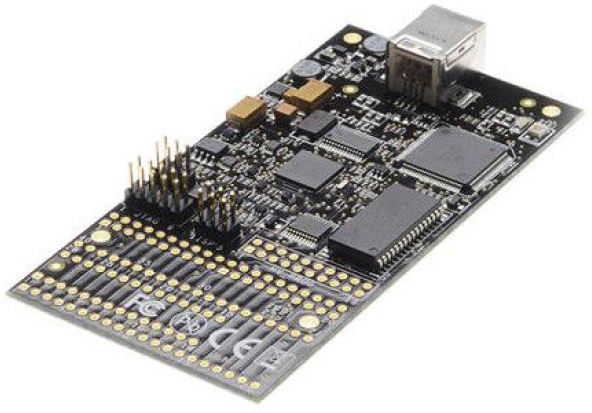
\includegraphics[width=\textwidth]{graphics/ISP/avr_dragon.PNG}
\captionof{figure}{AVR Dragon \cite{avrdragonug}}
\end{minipage}

\paragraph{Programmierinterface}
\label{para:programmierinterface}

Der AVR Dragon kann direkt mit dem Target Board, also der Wetterstation verbunden werden. Dafür werden vom AVR Dragon verschiedene Programmierinterfaces unterstützt: \cite{avrdragonug}\\

\begin{itemize}
	\item SPI Programming 
	\item High Voltage Serial Programming
	\item Parallel Programming
	\item JTAG Programming (\textit{D})
	\item PDI Programming (\textit{D})
	\item aWire Programming (\textit{D})
\end{itemize}
Jene, welche mit einem (\textit{D}) gekennzeichnet sind, dienen auch als Debugging Interface. In Bezug auf das Target Board wird der atmega2560 Mikrocntroller der Wetterstation über das SPI Interface programmiert. Der dafür vorgesehene SPI Header (6-Pin Header) ist auf dem AVR Dragon bereits gemounted, wodurch keine Lötarbeiten erforderlich sind (Abb. \ref{fig:spiheader}, rotes Rechteck).\\

\begin{center}
\begin{minipage}[b][7cm][t]{0.4\textwidth}
\centering
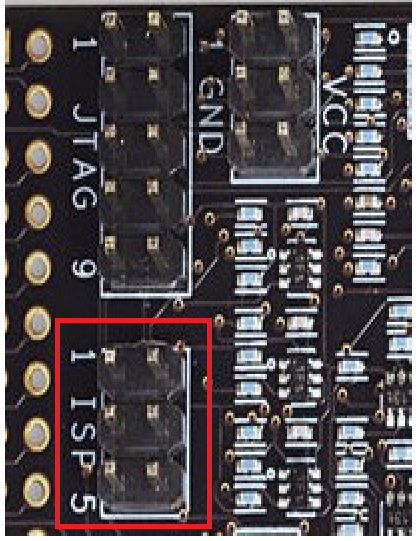
\includegraphics[height=6cm]{graphics/ISP/spi_header.PNG} 
\captionof{figure}{SPI Header \cite{avrdragonug}}
\label{fig:spiheader}
\end{minipage}
\begin{minipage}[b][7cm][t]{0.58\textwidth}
\centering
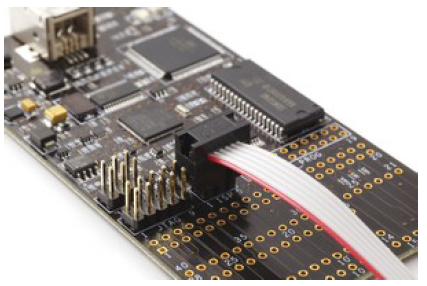
\includegraphics[height=6cm]{graphics/ISP/spi_header_anschluss.PNG} 
\captionof{figure}{Anschluss \cite{avrdragonug}}
\label{fig:spiheader_anschluss}
\end{minipage}
\end{center}

Beim Anschließen des Target Boards sollte darauf geachtet werden, dass die Speisespannung des Targets (3.3V) an dem Pin 2 des Headers angeschlossen ist. Somit kann der AVR Dragon mittels internem Level Converter alle Signale zwischen dem Target Board und sich selbst dem Target anpassen. Das Flachbandkabel sollte also wie in der Abbildung \ref{fig:spiheader_anschluss} angeschlossen werden.

\subparagraph{Zu Beachten:}
Da die $\mu$SD-Karte auf dem Target Board auch über das SPI Interface an den Mikrocontroller angeschlossen ist, so sollten die Jumper beim Anschließen entfernt werden. Es könnte zu Komplikationen führen, wenn Peripherie beim Flash-Vorgang noch an das SPI Interface angeschlossen ist.\\

\paragraph{Device Programming}
\label{para:device_programming}
Um auf das Target (Wetterstation) das Programm flashen zu könenn, müssen noch einige Dinge berücksichtigt werden. In diesem Kapitel wird das wichtigste in Kürze für das Device Programming erklärt. Die folgende Bildabfolge (Abb. \ref:{fig:deviceprogramming} bis \ref{fig:flashing}) soll den Ablauf veranschaulicht erklären und aufzeigen, worauf geachtet werden muss.\\

Als erstes muss das Device Programming über die Menübar \textit{Tools/Device Programming} geöffnet werden (Abb. \ref{fig:deviceprogramming}).\\

\begin{figure}[h]
\centering
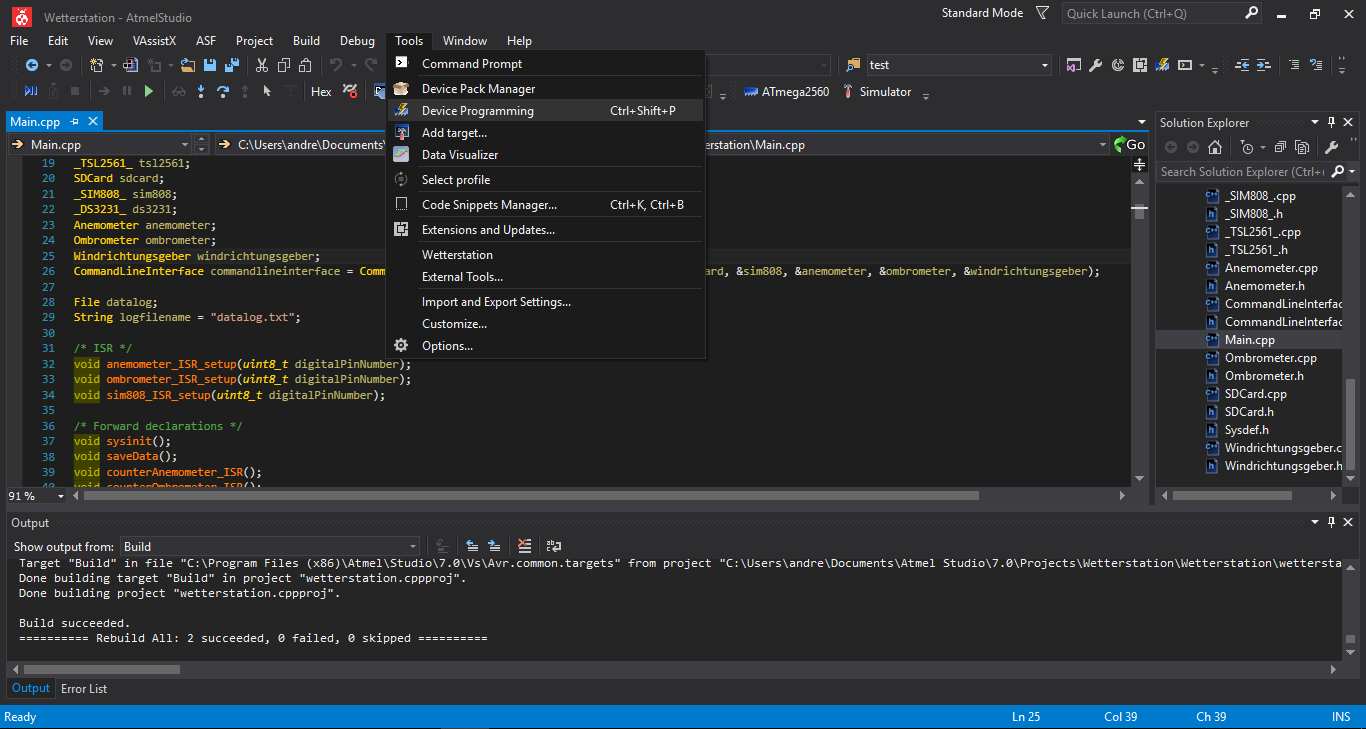
\includegraphics[width=0.7\textwidth]{../../../graphics/device_programming/1.PNG}
\caption{Auswahl Device Programming}
\label{fig:deviceprogramming}
\end{figure}
Wenn der AVR Dragon bereits per USB an den Computer angeschlossen wurde, dann sollte dieser bei Tool (oben links) auswählbar sein. Als Device selbst muss der ATmega2560 gewählt werden. Dies ist vom verwendeten Mikrocontroller abhängig. Das Programmier Interface ist ISP. In der Abbildung \ref{einstellung des ispclocks} ist noch zu sehen, dass der ISP Clock (Flash-Geschwindigkeit) einstellbar ist. Dieser sollte maximal einem Viertel der operierenden Taktfrequenz des Mikrocontrollers sein. In diesem Fall bei 8MHz Taktfrequenz also 2MHz.\\

\begin{figure}[h]
\centering
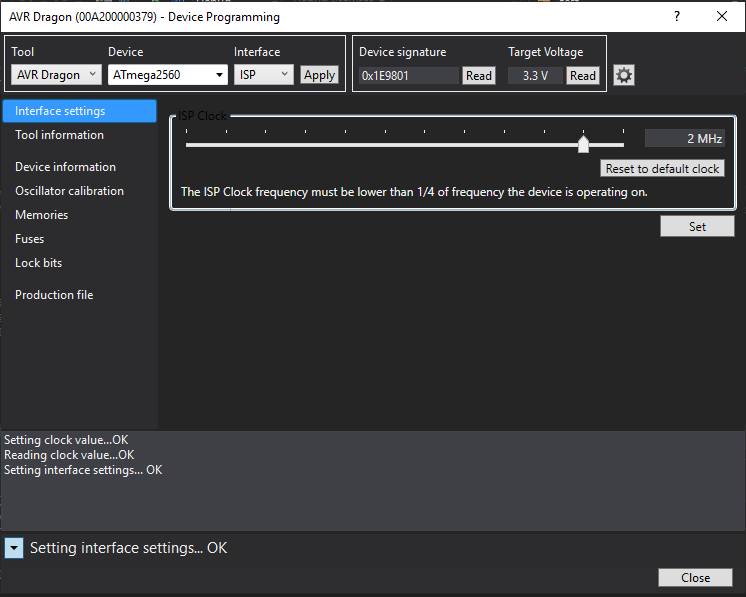
\includegraphics[width=0.7\textwidth]{../../../graphics/device_programming/2.PNG}
\caption{Einstellung des ISP Clocks}
\label{fig:einstellung des ispclocks}
\end{figure}
Für die Fuse Register (Abb. \ref{fig:fuseregister}) ist zu beachten, dass der Clockdivider \textit{LOW.CHKDIV8} abgewählt ist. Beim Kauf des Chips ist dieser oft default mässig eingeschaltet. Da auf dem Target ein externer Oscillator verwendet wird, muss auch dies hier angegeben werden. Dafür das Fuse Register \textit{LOW.SUT_CKSEL} auf einen externen Crystal Oscillator von 3.0 bis 8.0 MHz stellen. Anstatt alle Häckchen einzeln zu setzen, könnten die Values der Fuse Register auch direkt per Hexadezimalzahl angegeben werden. Somit werden alles nötige übernommen. Zum Schluss noch mit \textit{Program} bestätigen. Es können problemlos die Factory Settings überschrieben werden.\\

\begin{figure}[h]
\centering
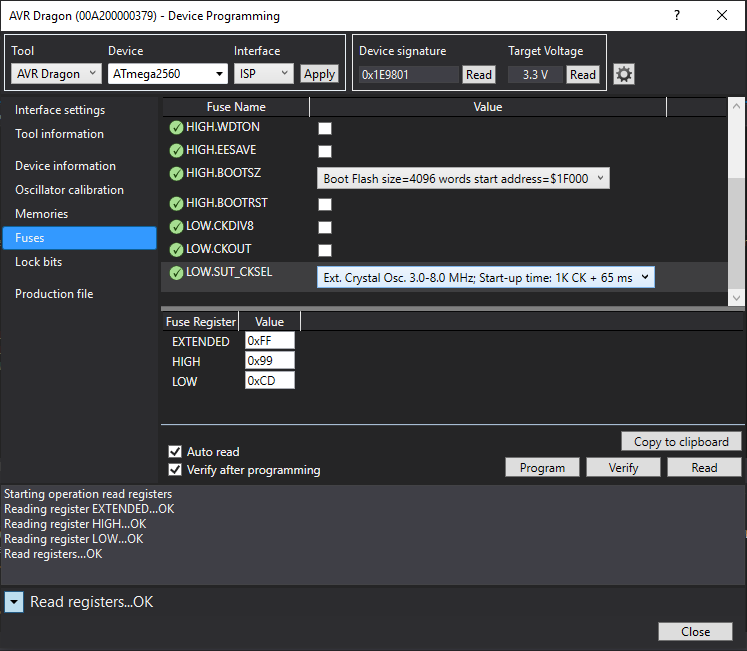
\includegraphics[width=0.7\textwidth]{../../../graphics/device_programming/3.PNG}
\caption{Fuse Register}
\label{fig:fuseregister}
\end{figure}
In der Abb. \ref{fig:lockbits} werden die Lock Bits gezeigt. Hier muss lediglich darauf geachtet werden, dass keine Lock Bits gesetzt werden. Das Lock Bit Register also auf 0xFF einstellen.\\

\begin{figure}[h]
\centering
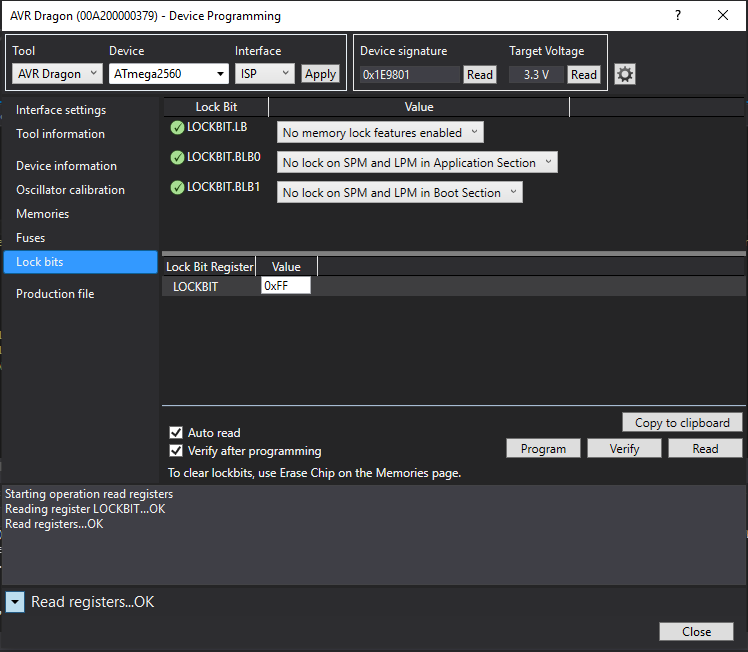
\includegraphics[width=0.7\textwidth]{../../../graphics/device_programming/4.PNG}
\caption{Lock Bits}
\label{fig:lockbits}
\end{figure}
Jetzt kann das geschriebene Programm auf den Mikrocontroller geflashed werden. Von Vorteil ist es, das Häckchen für \textit{Erase device before programming} zu setzen. Ansonsten muss dies jedes mal manuell vor dem Flashen durchgeführt werden. Zum Flashen den Button \textit{Program} drücken.\\

\begin{figure}[h]
\centering
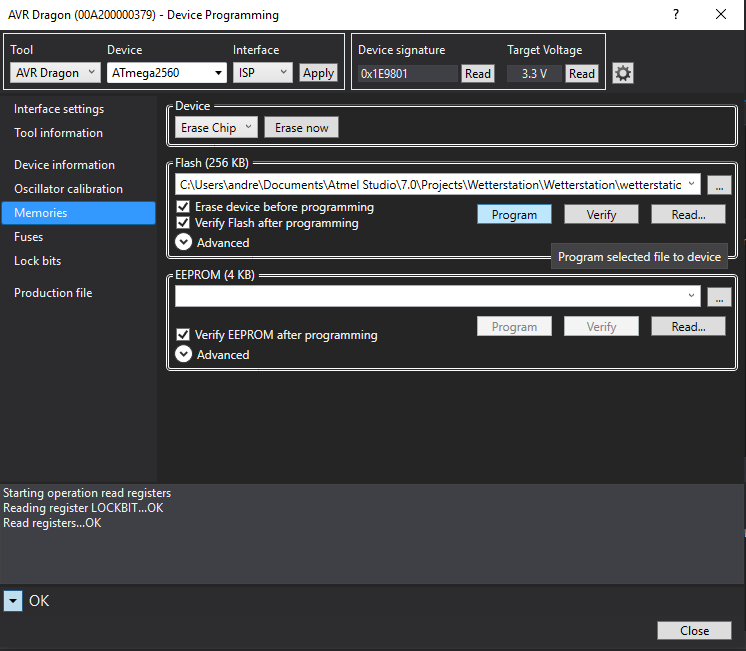
\includegraphics[width=0.7\textwidth]{../../../graphics/device_programming/5.PNG}
\caption{Flashing}
\label{fig:flashing}
\end{figure}

\subsection{UML-Diagramm}
\label{subsec:uml}

\begin{landsacpe}
\begin{figure}[h]
\centering
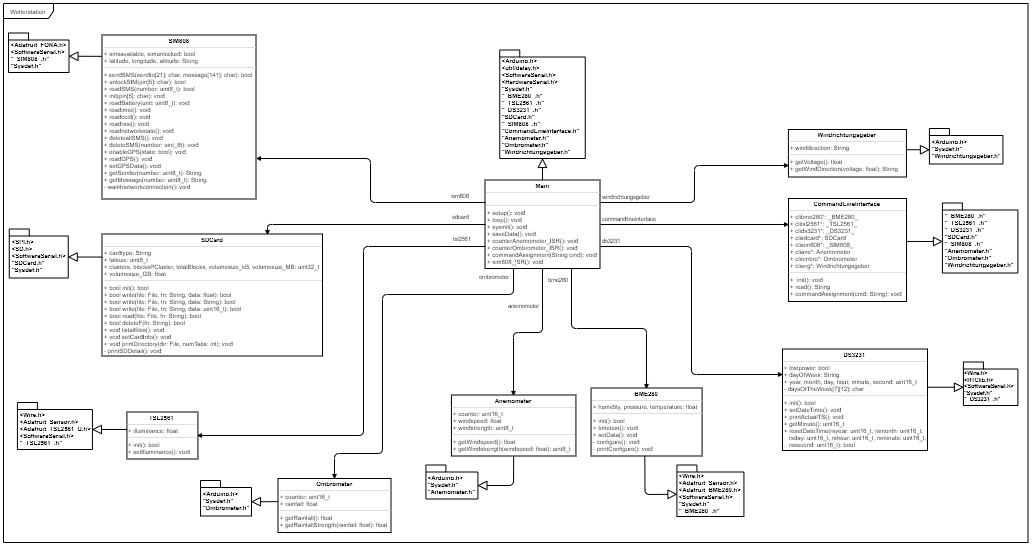
\includegraphics[width=0.9\textwidth]{../../graphics/UML/uml_diagramm_p6.PNG} 
\caption{UML-Diagramm}
\label{fig:uml_diagramm}
\end{figure}
\end{landscape}

Das in der Abbildung \ref{fig:uml_diagramm} dargestellte UML-Diagramm soll den Aufbau und die logischen Zusammenhänge der Firmware visualisieren. Darin wird gezeigt, welche Headerfiles bei den Klassen benötigt werden. Zudem sind die Attribute, wie auch die Funktionen mit ihren Access Specifier, Argumenten und Rückgabewerten aufgelistet. \\

\todo[inline]{Text überarbeiten. Ausführlich kurz das Programm erläutern}

Durch diese Struktur ist es möglich, adaptiv mehrere Komponenten hinzuzufügen und anzupassen. Zudem könnten somit auch mehrere Sensoren vom gleichen Typ ohne grossen weiteren Aufwand implementiert werden.\\

\subsubsection{Lizenzen}
\label{subsubsec:lizenzen}

Die verwendeten Librarys sind grundsätzlich aus der Arduino IDE von Arduino. Arduino selbst ist eine aus Soft- und Hardware bestehende Physical-Computing-Plattform, bei welcher beide Komponenten auf Open-Source-Basis quelloffen sind \cite{arduinoWiki}. Nach Aussage von Arduino selbst, stehen alle C/C++ Mikrocontroller Librarys unter der \textbf{LGPL} \cite{ArduinoLicense2019}. Einige Lizenz-Texte stehen im Anhang \ref{sec:lizenztexte}. \\

%Die RTClib steht unter der \textbf{MIT}-Lizenz, zusätzlich befindet sich noch der Lizenz-Text im Anhang \ref{subsec:rtclib_lizenztext}. Auch der Lizenz-Text der Adafruit_BME280 ist im Anhang \ref{subsec:adafruit_bme280_lizenztext}.\\

\begin{table}[h]
\centering
\caption{Lizenzen}
\label{tab:lizenzen}
\begin{tabular}{|l|l|l|}
\hline 
\textbf{Library} & \textbf{Author} & \textbf{Lizenz} \\ 
\hline 
Arduino & Arduino Team & LGPL V2.1 \\ 
\hline 
SPI & Cristian Maglie, Paul Stoffregen, Matthijs Kooijman, Andrew J. Kroll & LGPL V2.1 \\ 
\hline 
Wire & Nicholas Zambetti, Todd Krein, Chuck Todd & LGPL V2.1 \\ 
\hline 
SoftwareSerial & Limor Fried, Mikal Hart, Paul Stoffregen, Garrett Mace, Brett Hagman & LGPL V2.1 \\ 
\hline 
SD & SparkFun Electronics & GPL V3 \\ 
\hline 
RTClib & JeeLabs & - \\ 
\hline 
Adafruit\_Sensor & Kevin Townsend & Apache V2.0 \\ 
\hline 
Adafruit\_BME280 & Kevin Townsend & BSD \\ 
\hline 
Adafruit\_FONA & Limor Fried & BSD \\ 
\hline 
Adafruit\_TSL2561\_U & Kevin Townsend & BSD \\ 
\hline 
\end{tabular} 
\end{table}
\todo[inline]{Schreiben: SD GPL wegen sdfatlib. Es hat da zwei drin, File.cpp und SD.cpp. JeeLabs angeben mit link http://news.jeelabs.org/code/. Die The Android Open Source Project hat bei Adafruit Sensor das Copyright. Vielleicht hinzuschreiben. Und zum schluss noch den Text überarbeiten.}
\subsection{Validierung der Firmware}
\label{subsec:validierung_Firmware}
\subsection{Manual}
\label{subsec:manual}

\subsubsection{USB-to-Computer}
\label{subsubsec:usbtocomputer}

\subsubsection{SMS-Abfrage}
\label{subsubsec:smsAbrage}

\cleardoublepage
\thispagestyle{empty}
\vspace*{4cm}
\begin{center}
	\section{Hardware}
	\label{sec:Hardware}
\end{center}
\newpage
\subsection{Übersicht}
\label{subsec:Uebersicht}
Um eine bessere Vorstellung über die Wetterstation zu erhalten, wird hier das noch unbestückte PCB grafisch dargestellt und die verschiedenen Komponenten erläutert. Um die Übersichtlichkeit wahren zu können, werden in verschiedenen Bildern die Hauptbereiche mit einem roten Rahmen markiert und mit einer Zahl, jeweils neu beginnend bei 1, versehen. Wichtige Teilbereiche werden ebenfalls markiert und mit einem Buchstaben versehen, jeweils neu beginnend bei A.

\begin{figure}[h]
\centering
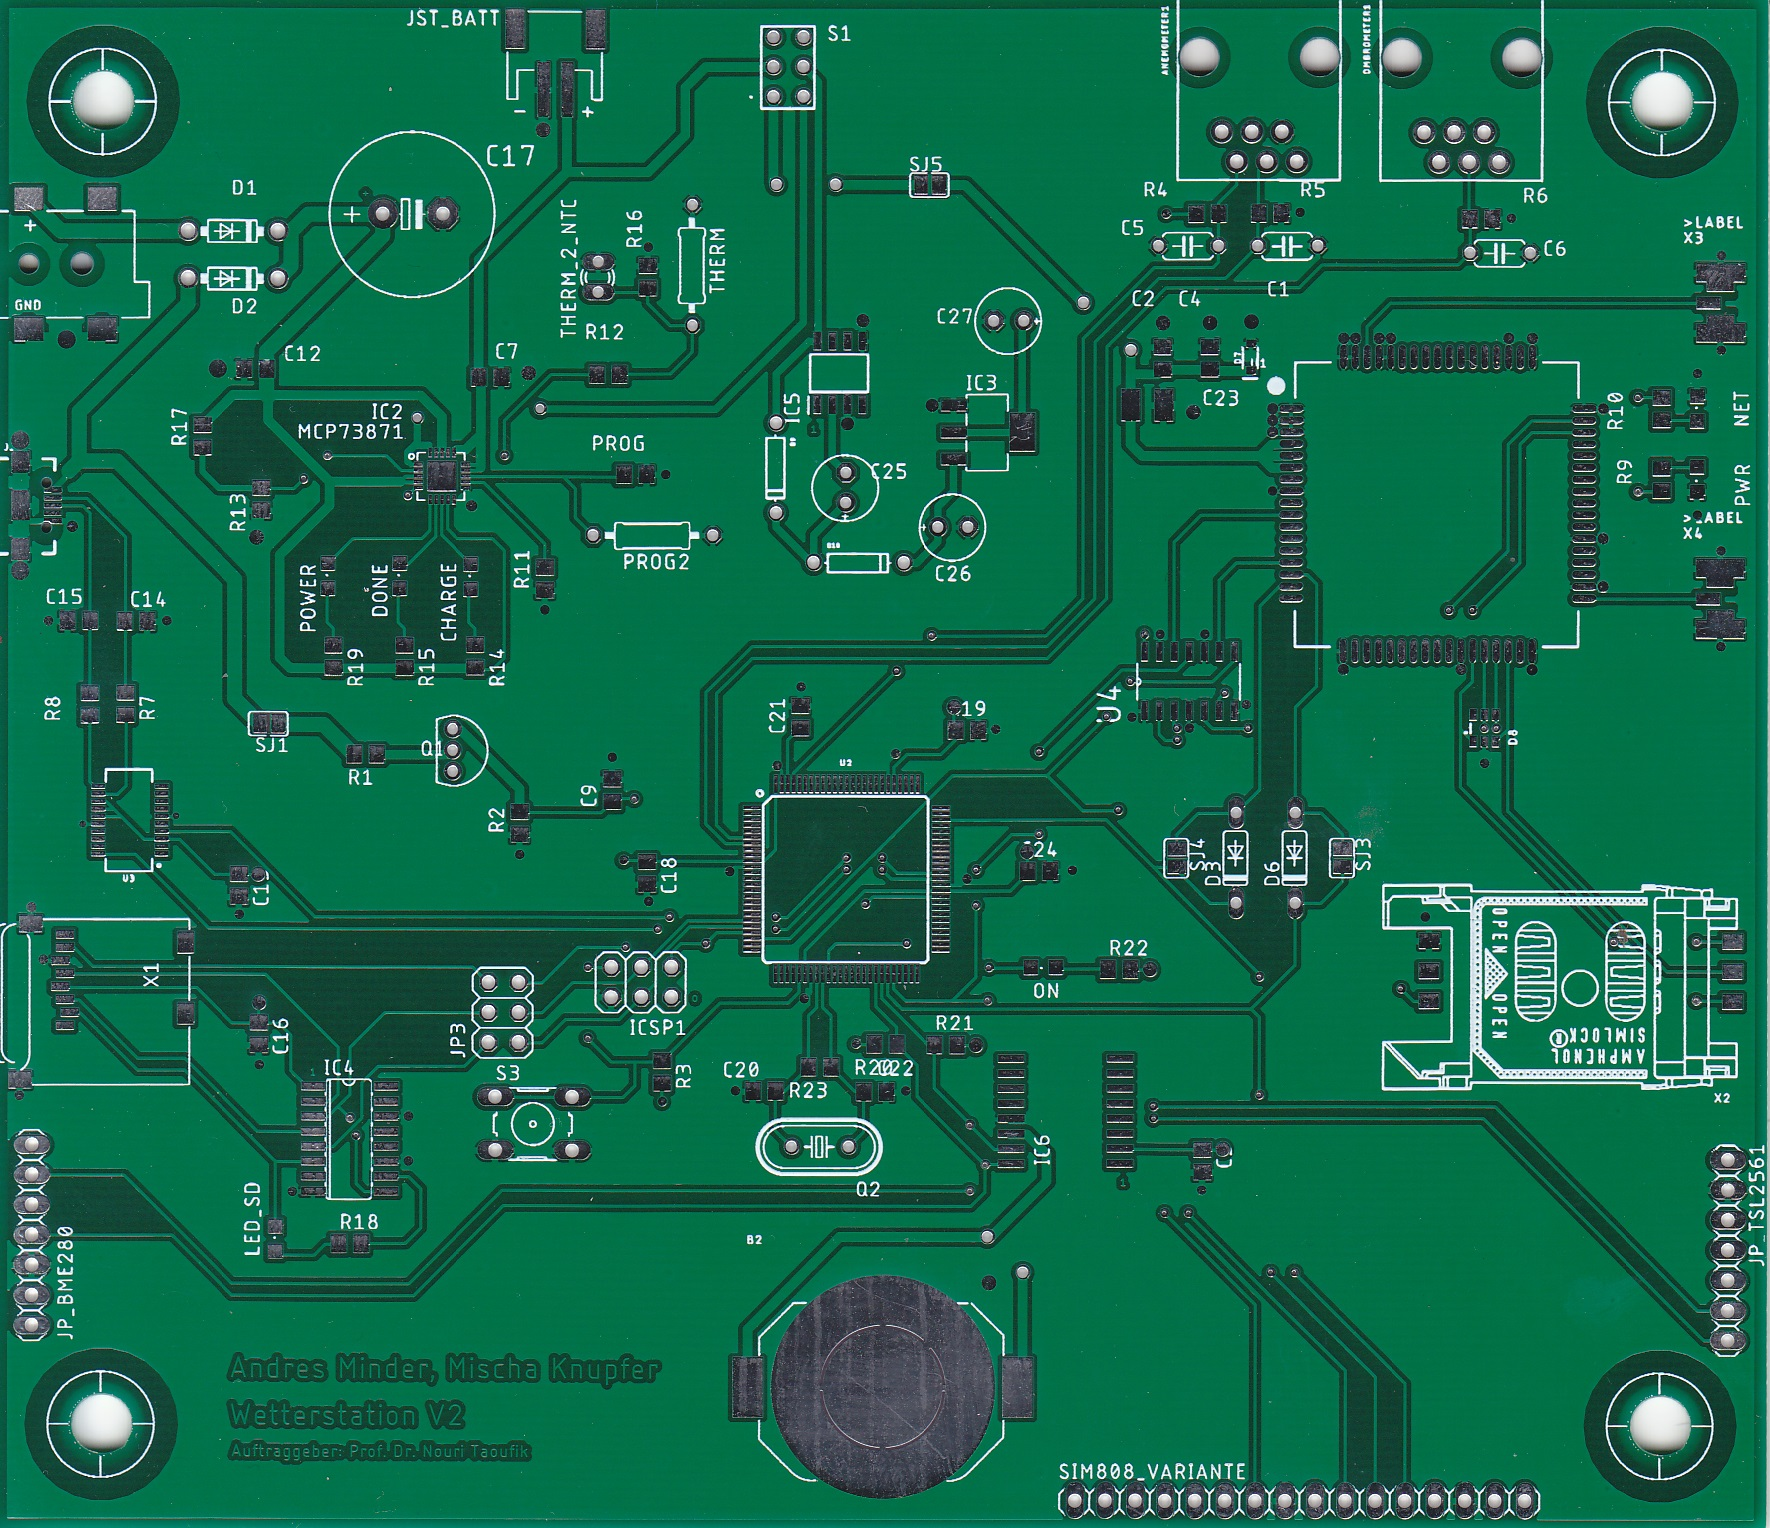
\includegraphics[width=0.99\linewidth]{graphics/HW_Uebersicht/PCB_Unbestueckt.jpg}
\caption{Das noch unbestückte PCB.}
\label{fig:Uebersicht_PCB_blank}
\end{figure}
Abbildung \ref{fig:Uebersicht_PCB_blank} zeigt das noch unbestückte PCB ohne markierte Bereiche. Man erkennt deutlich die Leiterbahnen sowie die Lötpads für die verschiedenen Bauteile. Welche Bauteile nun zur gleichen Bauteilgruppe gehören wird mit den nächsten Abbildungen erkenntlich.

\newpage

\begin{figure}[h]
\centering
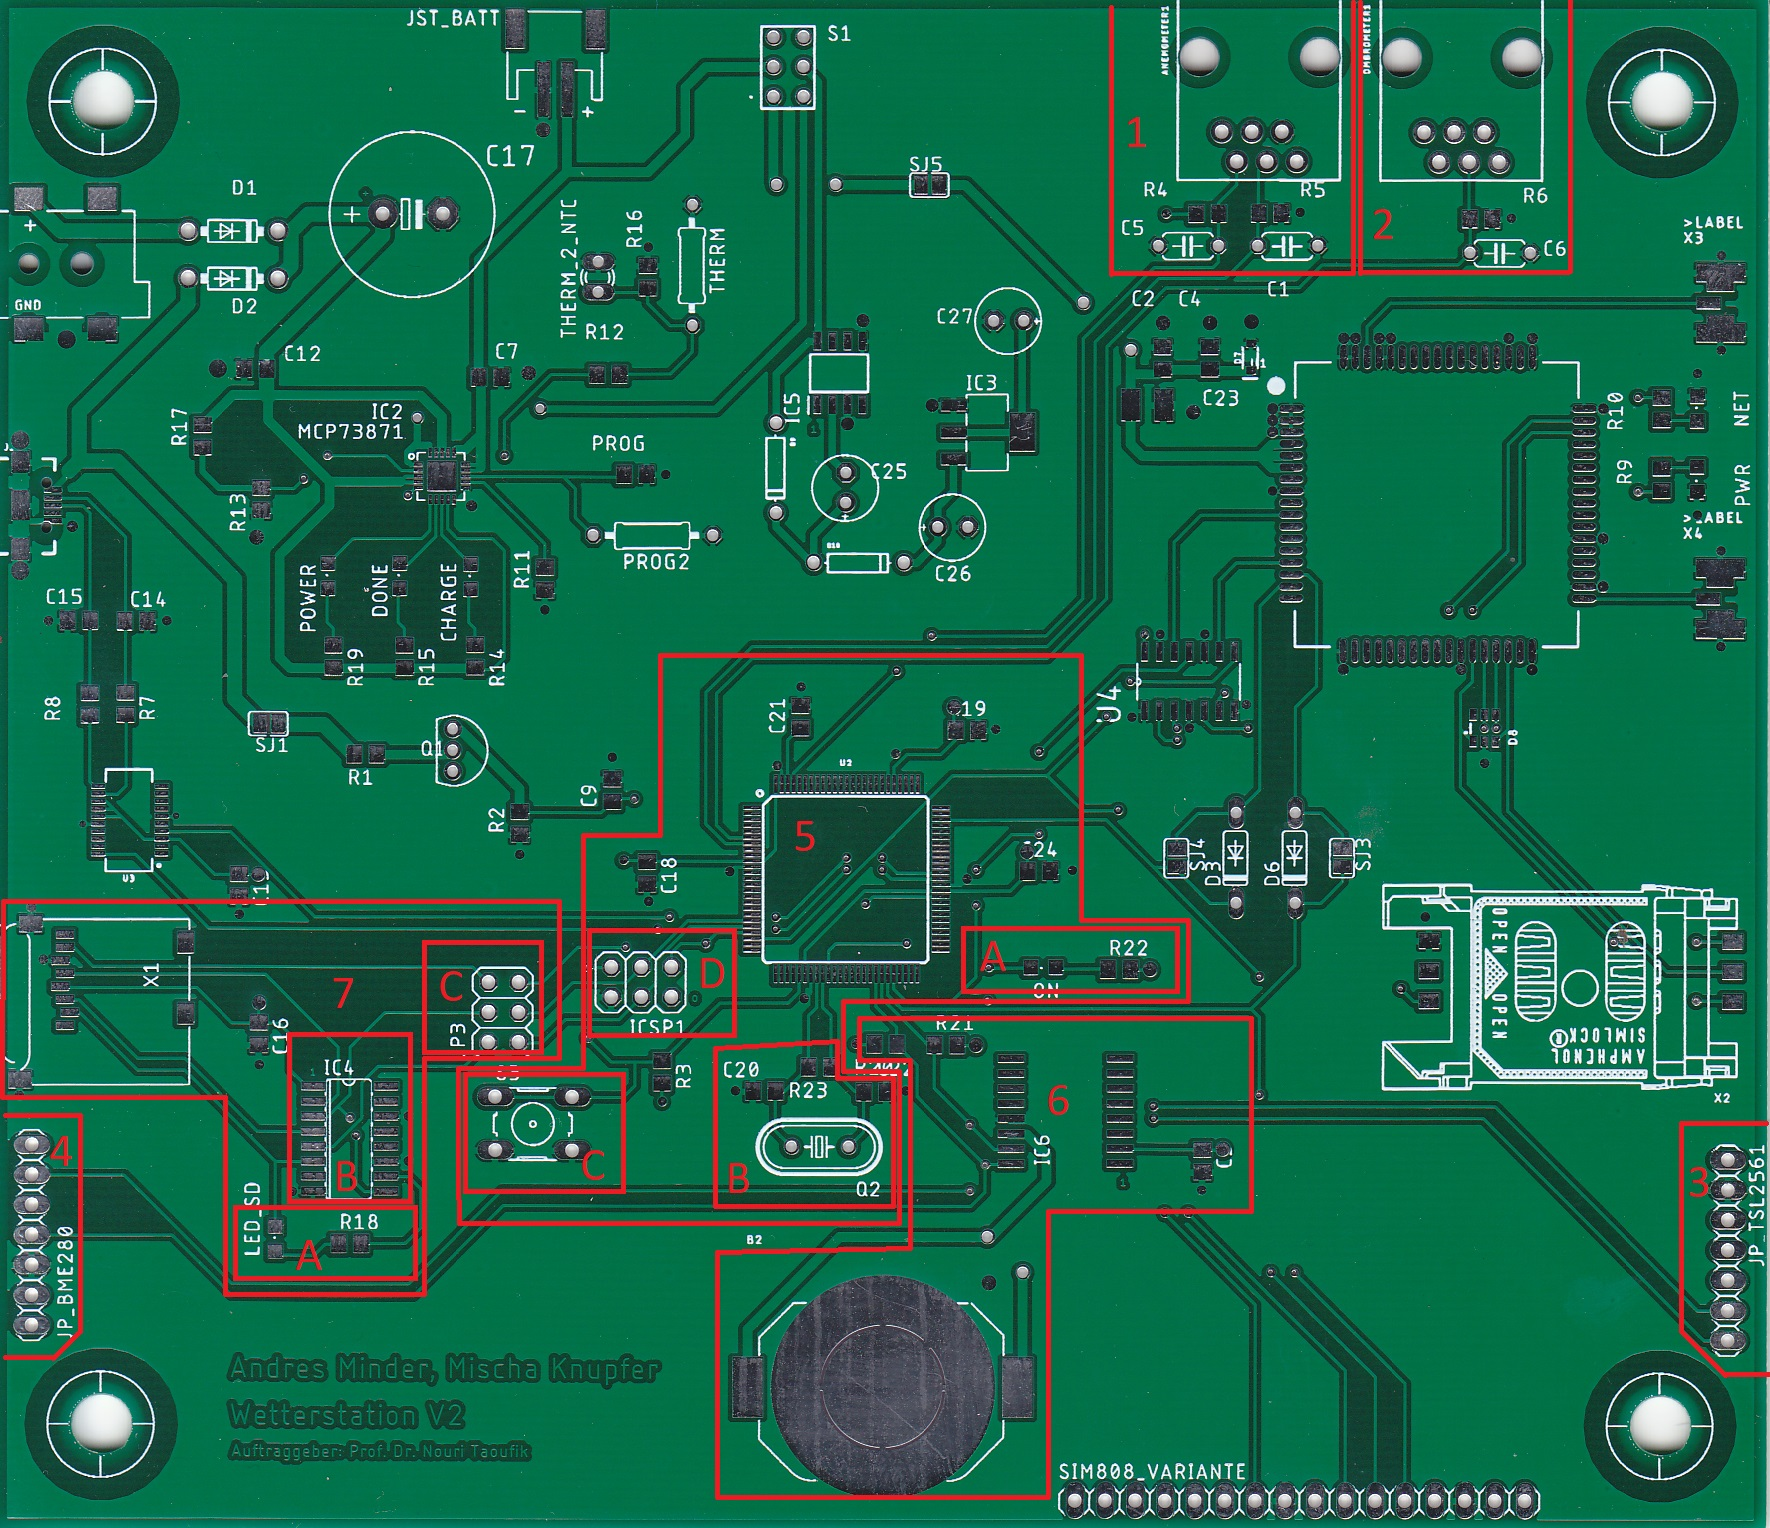
\includegraphics[width=0.99\linewidth]{graphics/HW_Uebersicht/PCB_Sensoren_MCU_SD_RTC.jpg}
\caption{Das unbestückte PCB mit den markierten Bereichen der MCU, der Datenspeicherung, der RTC und der Sensoren.}
\label{fig:Uebersicht_PCB_MCU_RTC_SD_Sense}
\end{figure}
Sieben Bauteilgruppen wurden in der Abbildung \ref{fig:Uebersicht_PCB_MCU_RTC_SD_Sense} markiert. Markierung 1 zeigt den RJ11-Stecker für das Anemometer mit Windrichtungsgeber, wobei an den Ausgängen jeweils ein RC-Filter angefügt wurde um Störungen im höheren Frequenzbereich herauszufiltern, um so ein nutzbares Signal zu erhalten. Das Ombrometer trägt die Markierung 2 und besitzt ebenfalls ein RC-Filter am Ausgang. Die 3 markiert die Pinleiste für den Anschluss des TSL2561 (Lichtintensitätssensor), ein nach aussen geführtes Breakout Board. Gleich Verhält es sich mit der 4, dem BME280. Die 5 markiert die Bauteilgruppe der MCU (ATMega2560), welche 4 wichtige Untergruppen beherbergt. 5-A zeigt eine Status-LED, welche leuchtet, sobald die MCU in betrieb ist. 5-B ist ein externer Clock, welcher der MCU den Takt vorgibt. Ein Reset der MCU und somit des Systems ist über den Reset-Button (5-C) möglich. Über 5-D, ein ICSP-Header (In Circuit System Programming), kann die MCU mit der Firmware geladen werden. Die 6 markiert die Bauteilgruppe des RTC (Real Time Clock) mit der zugehörigen Stützbatterie (CR2032 Knopfbatterie). Die 7-te Bauteilgruppe ist die Datenspeicherung. 7-A zeigt ein Status-LED, welche bei Aktionen mit der $\mu$SD-Karte aufleuchtet. 7-B beherbergt ein IC mit integrierten Operationsverstärkern, welche die Leitungen der $\mu$SD-Karte treiben. Über 5-C kann die Datenspeicherung über Jumper abgekoppelt werden, dies ist notwendig, da es während des Ladens der Firmware auf die MCU es sonst zu unkontrollierte Zugriffe auf die $\mu$SD-Karte kommen kann.

\begin{figure}[h]
\centering
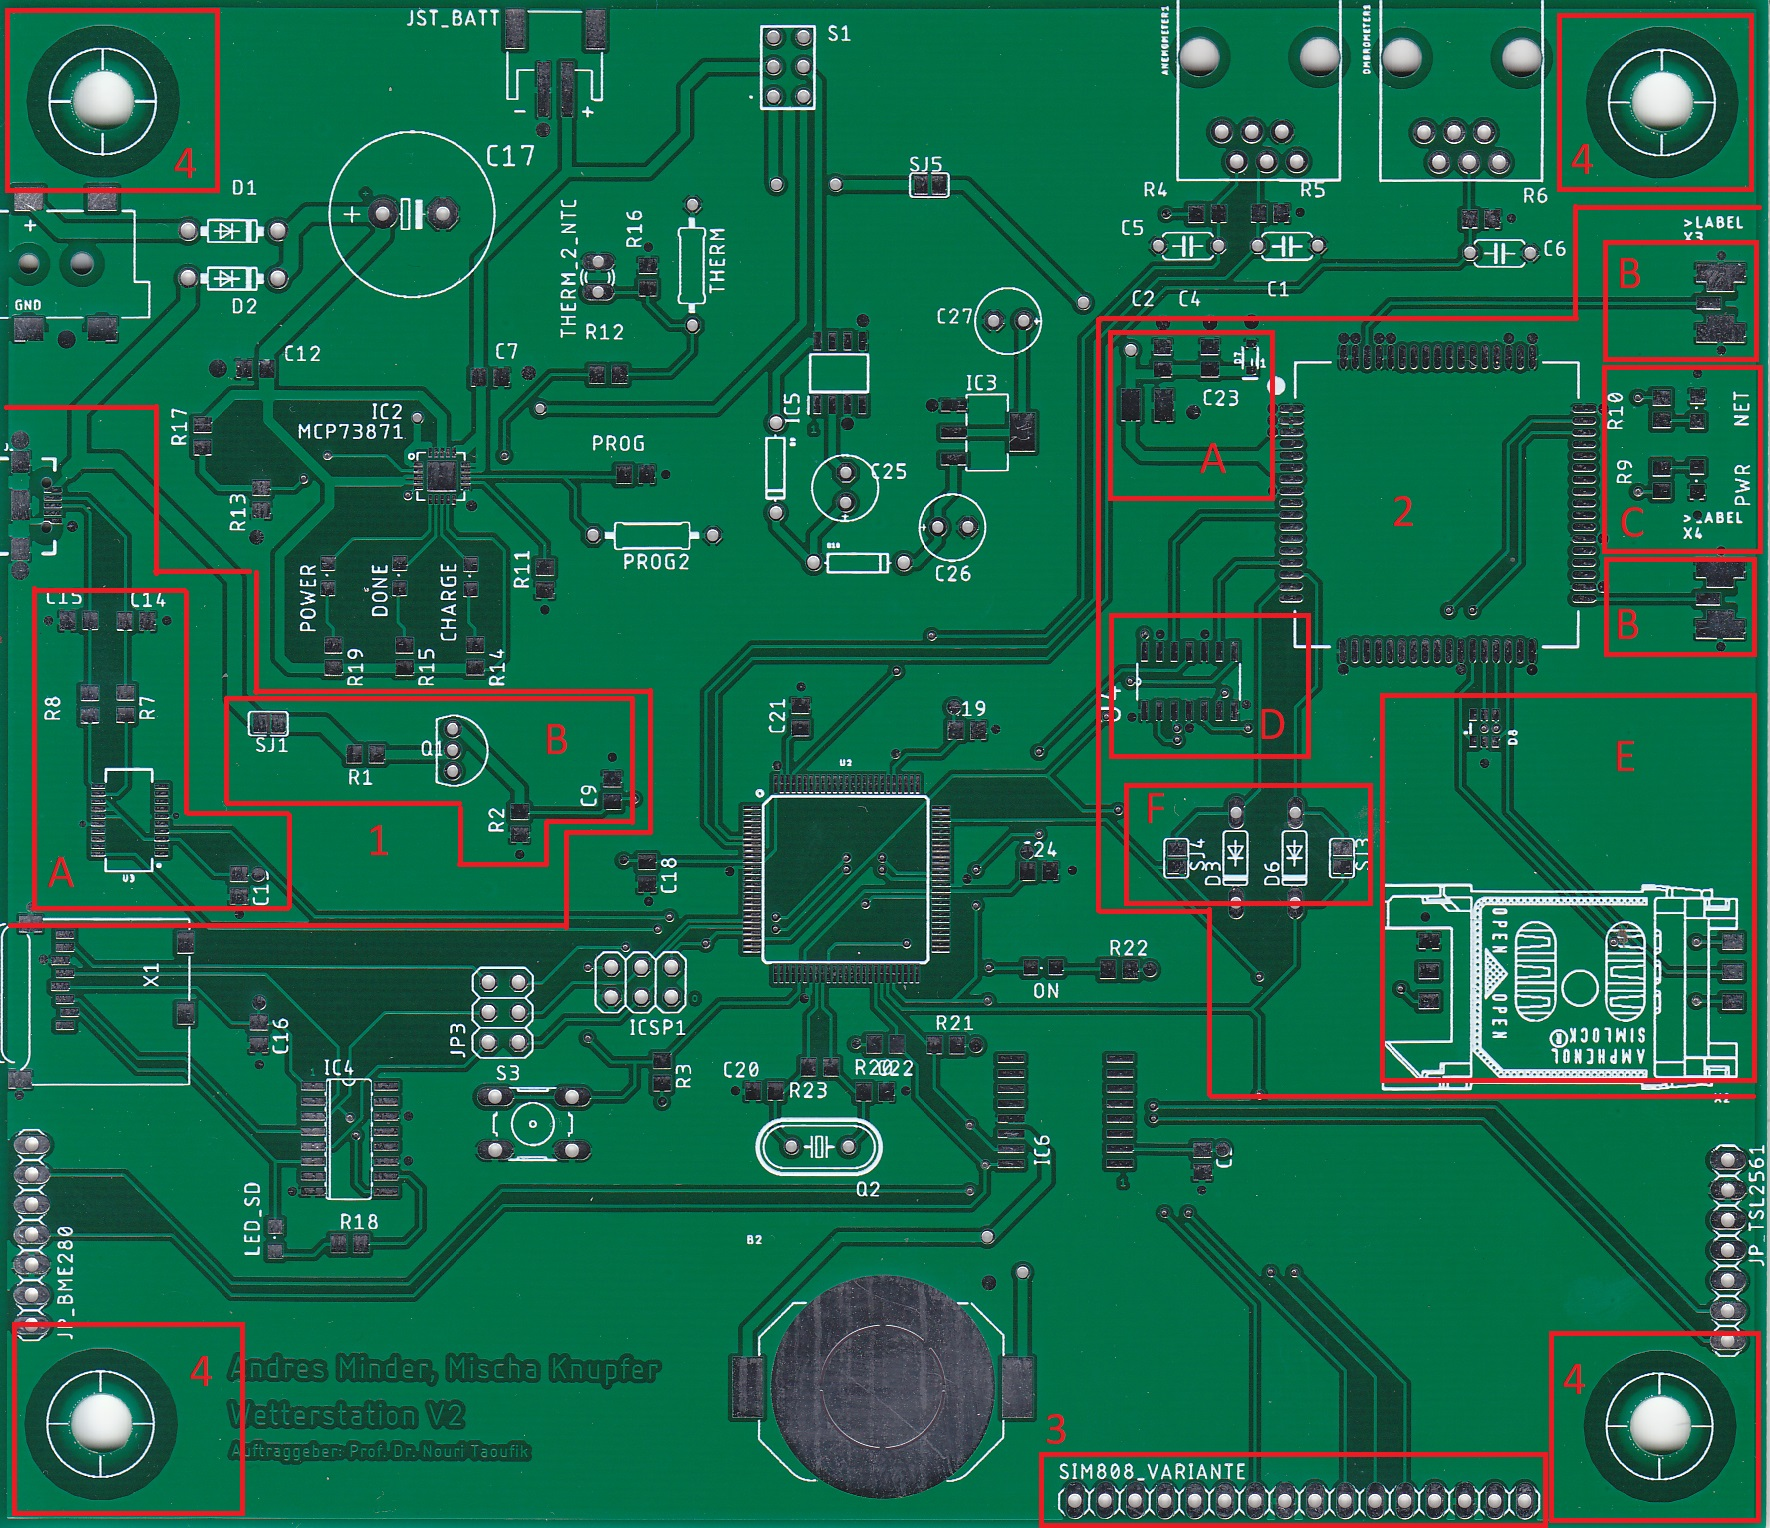
\includegraphics[width=0.99\linewidth]{graphics/HW_Uebersicht/PCB_USB_SIM808.jpg}
\caption{Das unbestückte PCB mit den markierten Bereichen des $\mu$USB-Interfaces, des SIM808 und der Bohrlöcher für die Montage im Gehäuse.}
\label{fig:Uebersicht_PCB_USB_SIM}
\end{figure}
Abbildung \ref{fig:Uebersicht_PCB_USB_SIM} zeigt die markierten Bereiche für die SIM808 (2), des $\mu$USB-Interfaces (1) und die Bohrlöcher für die Montage des PCBs im Gehäuse (4). Ausserdem gibt es eine Bestückungsvariante (3), bei der ein Breakout Board des SIM808 angeschlossen werden könnte, falls die On-Board Variante nicht funktionieren sollte. Im Bereich des $\mu$USB-Interfaces (1) sieht man deutlich zwei Teilbereiche, A und B. Teilbereich 1-A enthält den FT231XS, ein USB-to-UART IC, und dessen Beschaltung gemäss Datenblatt \cite{FTDI}. Für die Anschlusserkennung wird die Schaltung im Teilbereich 1-B verwendet. Für die SIM808 wird eine SIM-Karte (2-E) verwendet, sowie Antennen (2-C) und eine Schaltung zur Stabilisierung und Entstörung der Speisung (2-A) benötigt. 2-C beinhaltet zwei Status-LED, um den Betrieb und die Konnektivität anzuzeigen. Für die Anpassung des Spannungspegels vom 4V gespiesenen SIM808 auf die mit 3.3V gespiesene MCU dient der 74VHC125, zu sehen im Teilbereich 2-D. Zwei Dioden schützen den RST- und den RX-Pin des SIM808 vor ungewollten Spannungsspitzen und deren Folgen im Teilbereich 2-F.
\newpage

\begin{figure}[h]
\centering
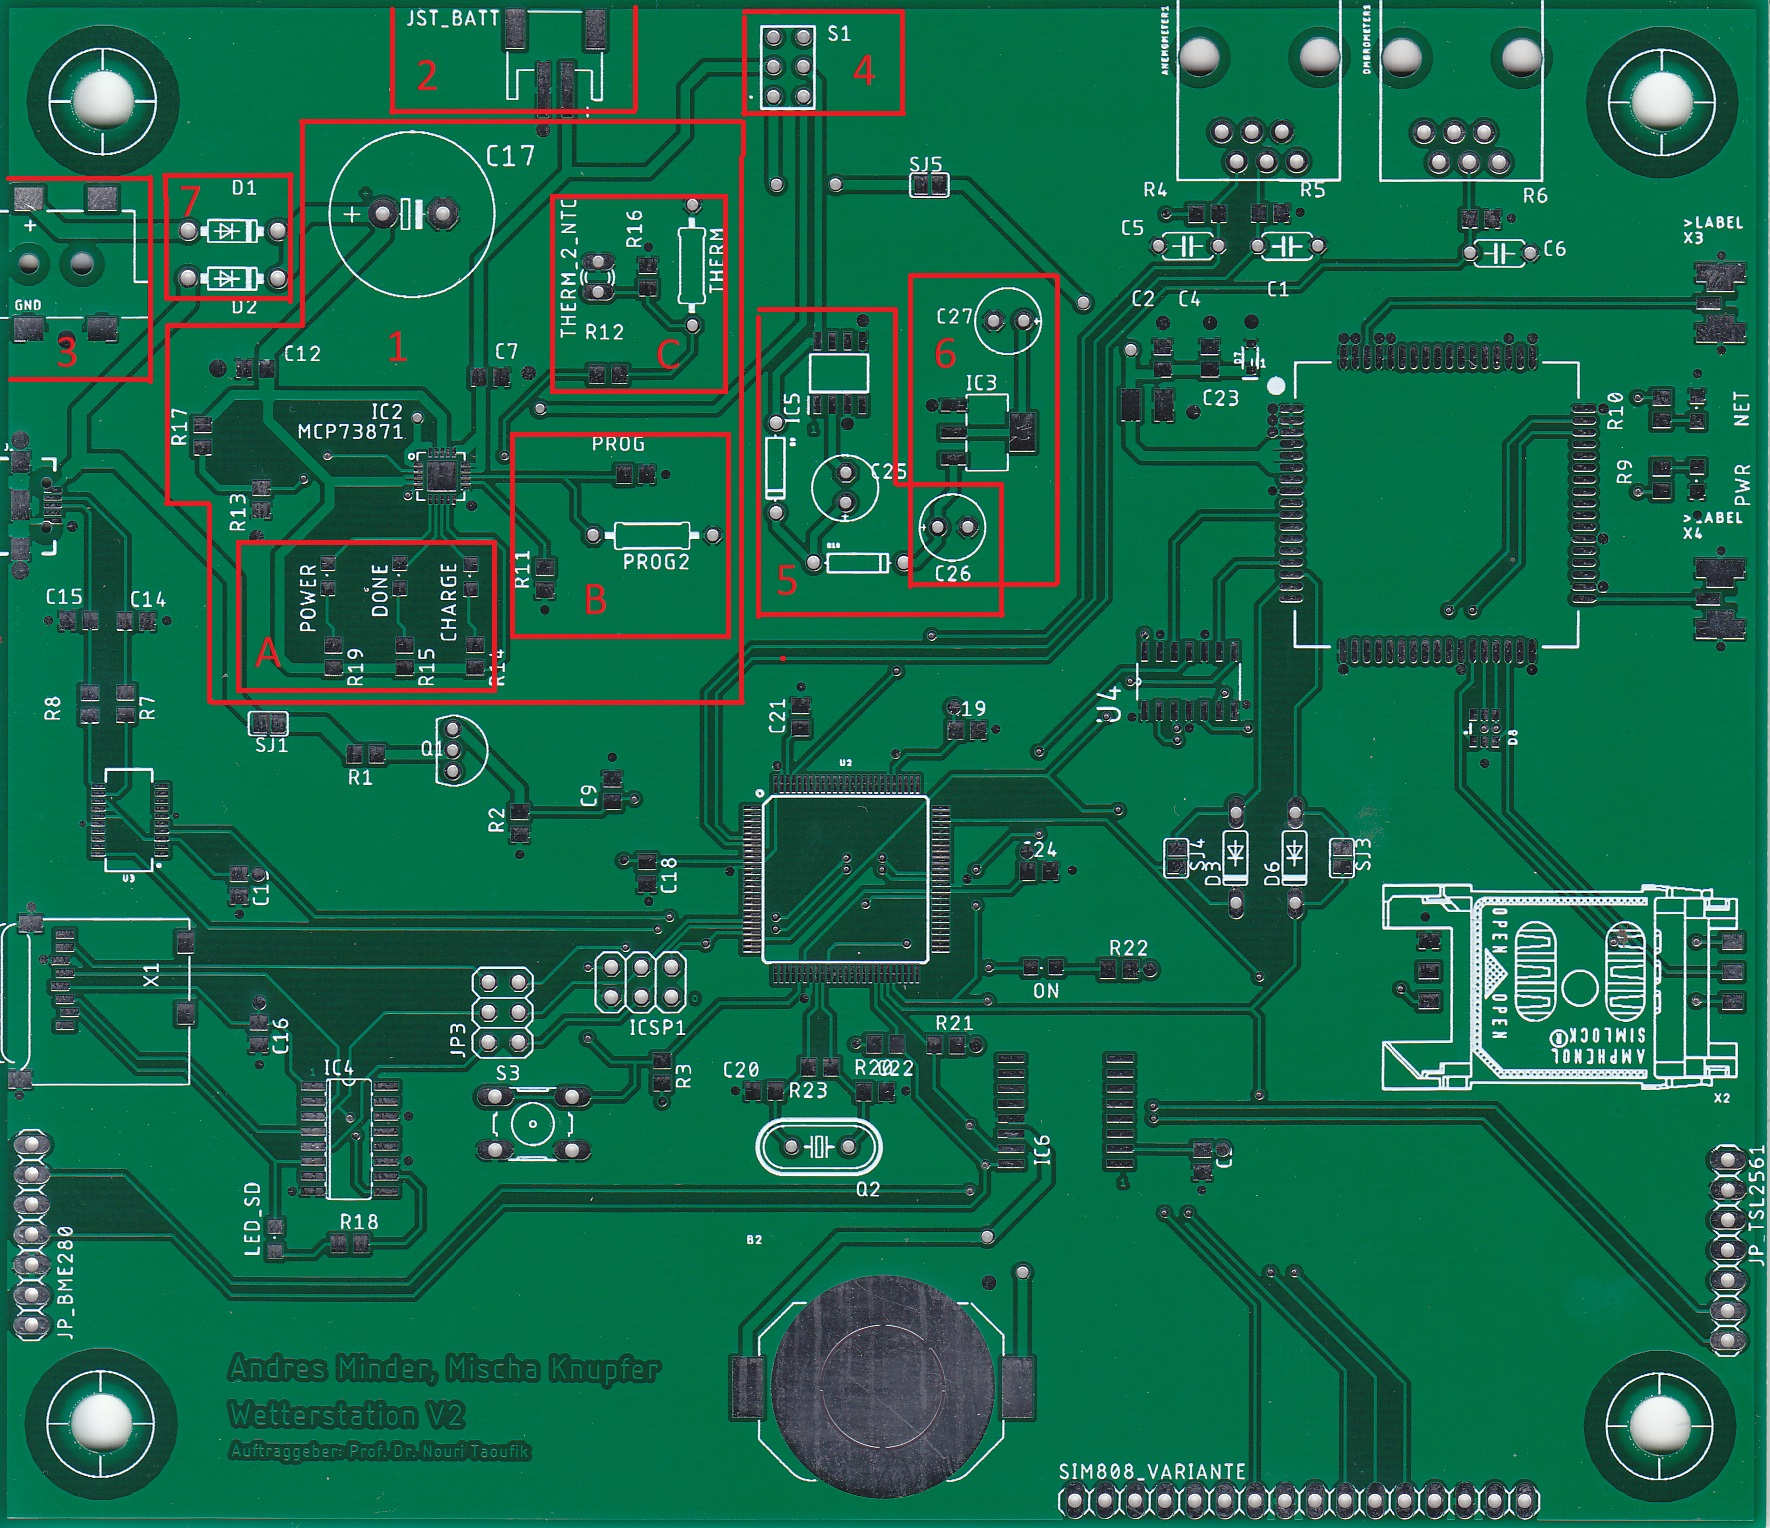
\includegraphics[width=0.99\linewidth]{graphics/HW_Uebersicht/PCB_Energieversorgung.jpg}
\caption{Das unbestückte PCB mit den markierten Bereichen für die Energieversorgung.}
\label{fig:Uebersicht_PCB_Energie}
\end{figure}
Die gesamte Schaltung für die Energieversorgung wurde in Abbildung \ref{fig:Uebersicht_PCB_Energie} in Bereiche unterteilt. Bereich 1 zeigt den MCP73871, den Power-Management-Chip, mit seinen Status-LED (1-A), sowie dessen Beschaltungen zur Einstellung des maximalen Ladestroms (1-B) und der Ausschalttemperatur (1-C). Der Anschluss für die Batterie erfolgt über den JST-Stecker (2). Über ein DC-Power Jack (3) wird die Photovoltaikanlage an die Wetterstation angeschlossen. Durch ein Schalter (4) können alle anderen Systeme der Wetterstation von der Energieversorgung getrennt werden. Die Charge-Pump (5) erhöht die erhaltene Batteriespannung, damit der Linearregler (6) die 3.3V-Ausgangsspannung mit möglichst kleinem Rippel erzeugen kann. Zwei Dioden (7) schützen die Eingänge vor rückfliessenden Strömen, indem diese nur in die gewünschte Richtung durchlassen und in die andere Richtung sperren.

In diesem Kapitel wurden die Bereiche des noch unbestückten PCBs erläutert und dadurch eine Übersicht über die Komponenten gegeben. In den nächsten Kapiteln soll auf diese Komponenten eingegangen werden, wobei mit der MCU begonnen wird.\\
\subsection{MCU}
\label{subsec:MCU}
Im Projekt 5 wurde bereits eine MCU ausgewählt, mit der das Prototyping erfolgte. Aufgrund der Verfügbarkeit (bei der FHNW bezugsbereit) wurde ein Arduino Mega2560 Board verwendet. Auf den kommenden bereits bestehenden Abschnitt aus dem Fachbericht des Projekt 5 folgt ein Abschnitt mit ergänzenden Informationen aus der Bachelor-Thesis.

\subsubsection{Bestehende MCU}
Die Micro Controller Unit (MCU) ist der zentrale Bestandteil für die Kommunikation, resp. für den Datenaustausch zwischen den unterschiedlichen Modulen. Sie interpretiert die Signale der Sensoren und rechnet sie in die interessierenden Messwerte um. Dann weist die MCU jedem Messwert einen Zeitstempel über das RTC zu und übergibt diesen der Datenspeicherung. Wenn die Daten vom Kommunikationsmodul angefordert werden, liest die MCU die Datenspeicherung aus und übergibt sie dem Kommunikationsmodul.\\

{\begin{minipage}[b][130pt][t]{0.5\textwidth}
Für die Entwicklung der MCU wird ein Arduino Mega Board verwendet. Der Vorteil besteht darin, dass elementare Bauteile (Hardware) bereits implementiert sind, wie z.B. Oszillator, der USB-Anschluss und die PCB-Connectors für ein schnelles Prototyping. Die wichtigsten technischen Daten sind in der Tabelle \ref{tab:arduinoMega_technischeDaten} aufgelistet.\\
\end{minipage}}
\hfill
{\begin{minipage}[b][130pt][t]{0.49\textwidth}
\centering
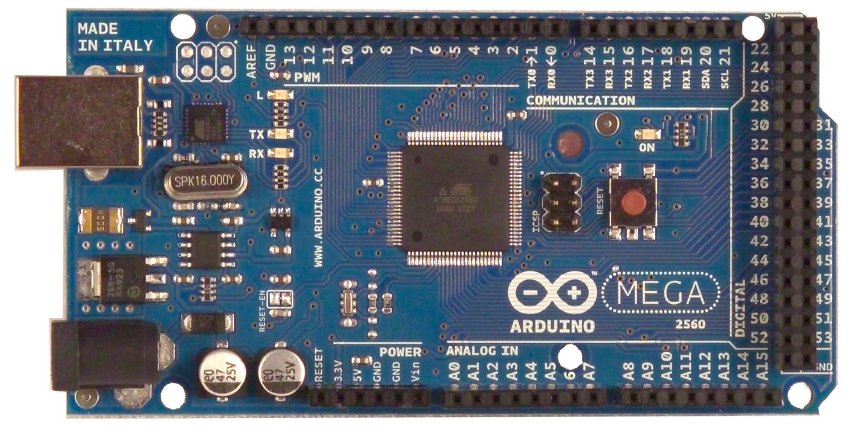
\includegraphics[width=0.99\textwidth]{graphics/MCU/arduino_mega.png}
\captionof{figure}{Arduino Mega Board \cite[S.1]{arduinoMega}}
\label{fig:arduinoMega}
\end{minipage}}

\begin{table}[h]
\centering
\caption{Technische Daten \cite[S.3]{arduinoMega}}
\begin{tabular}{|l|l|}
\hline 
Microcontroller & ATmega2560 \\ 
\hline 
Operating Voltage & 5V \\ 
\hline 
Digital I/O Pins & 54  \\ 
\hline 
Analog Input Pins & 16 \\ 
\hline 
Flash Memory & 256 KB, 8 KB werden vom bootloader benötigt\\ 
\hline 
SRAM & 8 KB \\ 
\hline 
EEPROM & 4 KB \\ 
\hline 
Clock Speed & 16 MHz \\ 
\hline 
\end{tabular}
\label{tab:arduinoMega_technischeDaten}
\end{table}
\newpage
\subsubsection{Ergänzungen aus der Bachelor-Thesis}
{\begin{minipage}[b][220pt][t]{0.55\textwidth}
Während der Bachelor-Thesis kam die Idee auf, eine kleinere MCU zu verwenden. Eine kleinere MCU hat die Vorteile, dass diese günstiger ist in der Anschaffung, einen geringeren Stromverbrauch aufweist und weniger Platz auf dem PCB benötigt.  Aufgrund der Firmware wird jedoch eine erhöhte Menge Speicher alloziert, weshalb die \textit{Data Memory Usage} des verwendeten ATMega328 zu klein war und wieder auf den bereits für das Prototyping verwendeten ATMega2560 zurückgegriffen werden musste. Für die Wetterstation wird schlussendlich kein Board mehr verwendet, sondern der Mikroprozessor (ATMega2560, siehe Abbildung \ref{fig:ATMega2560}) selbst auf dem PCB platziert. Damit dieser wie gewünscht funktioniert, werden weitere Bauteile verwendet. Im nächsten Abschnitt wird mehr auf die zusätzlichen Bauteile eingegangen.
\end{minipage}}
{\begin{minipage}[b][220pt][t]{0.44\textwidth}
\centering
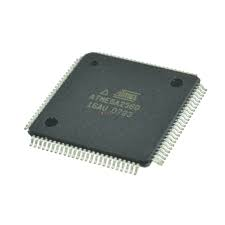
\includegraphics[width=0.8\linewidth]{graphics/MCU/ATMega2560.jpg}
\captionof{figure}{Der Mikroprozessor ATMega2560, ohne Board.}
\label{fig:ATMega2560}
\end{minipage}}

Wie in der Übersicht in Abbildung \ref{fig:Uebersicht_PCB_MCU_RTC_SD_Sense} zu sehen ist, wird für die MCU ein ICSP-Header (In Circuit System Programming) benötigt. Durch diesen ICSP-Header kann die Firmware über ein AVR-Dragon auf die MCU geladen werden, wobei spätere Anpassungen der Firmware möglich bleiben, was wiederum zur Skalierbarkeit (Erweiterbarkeit) des Systems beiträgt. Die MCU selbst (ATMega2560) hat einen internen Clock, welcher über ein RC-Oszillator generiert wird und eine wesentlich höhere Temperaturabhängigkeit besitzt als ein externer Quarz. Aus diesem Grund wird ein externer Quarz verwendet, wie in Abbildung \ref{fig:Uebersicht_PCB_MCU_RTC_SD_Sense} ebenfalls ersichtlich ist. Ausserdem werden Kondensatoren bei den 3.3V-Speisepins verwendet, um Induktivitäten durch Leiterbahnlängen auszugleichen. Um das System rebooten zu können wird ein Reset-Button hinzugefügt, wobei über eine Status-LED der Betrieb der MCU ersichtlich ist. Über ein CLI (Command Line Interface) soll mit der MCU interagiert werden können, wodurch eine Verbindung mit einem $\mu$USB-Interface erforderlich wird. Die Sensorik, die RTC (Real Time Clock) und die SIM808 werden ebenfalls mit der MCU verbunden, was die MCU zum Herzstück der Wetterstation macht, da hier alle Daten verarbeitet werden. Die verarbeiteten Daten werden in der angeschlossenen Datenspeicherung wiederum gespeichert.\\[0.5cm]
In diesem Kapitel wurde die Thematik der MCU eingehend thematisiert. RC-Oszillatoren und Quarze wurden ebenfalls erwähnt. Aus diesem Grund wird im nächsten Kapitel die RTC näher erläutert.

\subsection{RTC}
\label{subsec:RTC}
Im vergangenen Kapitel (MCU) wurden bereits RC-Oszillatoren und Quarze erwähnt. Die RTC (Real Time Clock) beinhaltet ebenfalls einen Quarz, weshalb die RTC in diesem Kapitel näher erläutert wird.
Die RTC wurde bereits während des Projekt 5 integriert und in dessen Fachbericht dokumentiert. Nachfolgender, bereits bestehender Text wurde übernommen.

\subsubsection{Bestehende RTC}
Um die gewonnenen Messdaten mit einem Zeitstempel zu versehen, wird eine \textbf{RTC} (\textit{real time clock}) benötigt. Um eine möglichst kleine Abweichung zu haben, wird eine hohe Präzision vorausgesetzt. Ausserdem soll die \textbf{RTC} über das in Kapitel \ref{chap:Interfaces} erwähnte \textbf{I$^2$C}-Bus angesteuert werden. Aus diesen Gründen wurde der \textbf{DS3231} implementiert, da dieser als Präzisions-\textbf{I$^2$C}-\textbf{RTC} die Anforderungen erfüllt. Die hohe Präzision des \textbf{DS3231} wird mit einem internen Temperatursensor erreicht, welcher Temperaturbedingte Abweichungen des Oszillators kompensiert. Zu sehen ist der \textbf{DS3231} mit seinen Anschlüssen in Abbildung \ref{fig:DS3231}.

\begin{figure}[h]
\centering
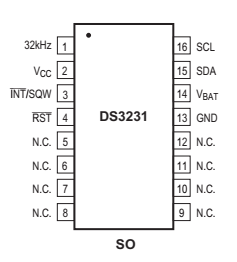
\includegraphics[width=0.4\linewidth]{graphics/DS3231.png}
\caption{DS3231 mit seinen Anschlüssen \cite{DS3231DS}.}
\label{fig:DS3231}
\end{figure}

Die Anschlüsse des \textbf{DS3231} sind \textbf{VCC}, \textbf{GND}, \textbf{SCL}, \textbf{SDA}, \textbf{BAT}, \textbf{32K}, \textbf{SQW} und \textbf{RST}. \textbf{VCC} und \textbf{GND} werden für die Speisung benötigt. \textbf{SCL} und \textbf{SDA} sind Anschlüsse für den \textbf{I$^2$C}-Bus. \textbf{BAT} ist der positive Anschluss der Knopfbatterie, worüber deren Zustand kontrolliert werden, etwas anderes gespiesen oder eine andere Battery als Backup angeschlossen werden kann. \textbf{32K} ist ein Anschlusspin um den Output des 32kHz-Oszillators des \textbf{RTC} abzugreifen, was jedoch nicht verwendet wird. \textbf{SQW} ist ein zusätzlicher Output- oder Interrupt-Pin, welcher jedoch auch nicht verwendet wird. \textbf{RST} wird verwendet, um ein externes Element zu reseten oder als Indikator wenn die Hauptspeisung unterbrochen wird. \cite{DS3231DS}\\

\newpage
Die relevanten Spezifikationen des Chips sind in Tabelle \ref{tab:DS3231} aufgelistet.\\

\begin{table}[h]
\begin{tabular}{llllll}
\hline 
\textbf{Parameter} & \textbf{Min.} & \textbf{Typ.} & \textbf{Max.} & \textbf{Einheit} & \textbf{Condition} \\ 
\hline 
VCC & 2.3 & 3.3 & 5.5 & V &  \\ 
VBAT & 2.3 & 3 & 5.5 & V &  \\ 
Active Supply Current &  &  & 200 & $\mu$A & 3.63 V \\ 
 &  &  & 300 & $\mu$A & 5.5 V \\ 
Standby Supply Current &  & & 110 & $\mu$A & 3.63 V \\ 
 &  &  & 170 & $\mu$A & 5.5 V \\ 
Crystal Aging &  & $\pm$ 1 &  & ppm & First Year \\ 
 &  & $\pm$ 5 &  & ppm & 0-10 Years \\ 
Active Battery Current &  &  & 70 & $\mu$A & 3.63 V \\ 
 &  &  & 150 & $\mu$A & 5.5 V \\ 
Timekeeping Battery Current &  & 0.84 & 3 & $\mu$A & 3.63 V \\ 
 &  & 1 & 3.5 & $\mu$A & 5.5 V \\ 
\hline 
\end{tabular} 
\caption{Spezifikationen des DS3231 \cite{DS3231DS}.}
\label{tab:DS3231}
\end{table}

Tabelle \ref{tab:DS3231} zeigt die für das Projekt relevanten Spezifikationen des \textbf{DS3231}. Wichtig ist, dass die Alterung des Quarzes zu einem Fehler führt, dieser jedoch im ppm-Bereich liegt und somit erst über viele Jahre hinweg bemerkbar wird.\\[0.5cm]
Wie erwähnt wurde, wird die RTC über den I$^2$C-Bus von der MCU angesteuert. Da dies ebenfalls für gewisse Sensoren gilt, werden im nächsten Kapitel die Sensoren thematisiert.

%\subsection{Implementation in die Firmware}
%Für die Implementation wurde die bereits existierende Library \textbf{RTClib} von Adafruit in die Firmware integriert. Anschließend konnte das Headerfile <Adafruit\_RTClib.h> inkludiert werden und mit der Funktion \textit{TimeStamp getTimeStamp()} der aktuelle Zeitstempel abgerufen werden. \\
%Beim flashen des Programms wird die RTC mit der Uhr des angeschlossenen Computers synchronisiert, weshalb es durch die Übertragungsverzögerung zu einer Abweichung kommt, welche der Dauer des flashens entspricht.

\subsection{Bestehende Sensorik}
\label{subsec:Sensoren}
Der grossteil der Sensorik wurde bereits während des Projekt 5 implementiert und in dessen Fachbericht dokumentiert. Die Dokumentation der bereits implementierten Sensorik wird in nachfolgendem Abschnitt inkludiert und darauf folgend die während der Bachelor-Thesis hinzugekommene Sensorik bzw. Ergänzungen in einem separaten Abschnitt erläutert.

\subsubsection{Ombrometer}

\subsubsection*{\textbf{Ermittlung der Niederschlagsmenge}}
Dieses Unterkapitel befasst sich mit der Realisierung der Niederschlagsmessung. Diese soll nach einem Kipplöffelprinzip funktionieren und gemäss definierten Zielen eine Genauigkeit von $\pm$100 ml/$m^2$ aufweisen. Ausserdem soll als alternative zusätzlich ein Messbecher an der Wetterstation installiert werden, damit der Bauer die Niederschlagsmenge anhand einer Skala ablesen kann. In einem ersten Schritt soll das Kipplöffelprinzip näher erläutert und mit einem Selbstbau die Funktionsweise getestet werden. Anschliessend soll ein gekaufter Sensor die Wetterstation erweitern und die Implementation in der Firmware thematisiert werden. Zu guter Letzt soll die Validierung des Teilsystems folgen.
\subsubsection*{\textbf{Das Kipplöffelprinzip}}
Das Prinzip des Kipplöffels wird in Abbildung \ref{fig:Kipp} graphisch dargestellt.

\begin{figure}[h]
\centering
\includegraphics[width=0.8\linewidth]{graphics/Kipploeffel.png}
\caption{Darstellung des Kipplöffelprinzips}
\label{fig:Kipp}
\end{figure}

Abbildung \ref{fig:Kipp} zeigt das Kipplöffelprinzip. Der Kipplöffel (\glqq 3)\grqq) besteht im Grunde aus zwei Löffeln und ist in der Mitte drehbar mit dem Gehäuse befestigt (\glqq 4)\grqq). Regenwasser wird über eine Öffnung im Gehäusedeckel (Trichter, \glqq 1)\grqq) zum Kipplöffel befördert (\glqq 2)\grqq). Ist der Löffel mit Regenwasser gefüllt, so kippt dieser aufgrund des Gewichts und leert das Wasser über eine Öffnung im Gehäuseboden (\glqq 5)\grqq) aus. Durch die Kippung wird der andere Löffel in die Ausgangsposition bewegt und kann sich nun mit Wasser füllen. Mit der Hilfe von Reedkontakten und Magneten wird die Anzahl der Kippbewegungen gezählt. Die Niederschlagsmenge ergibt sich aus der Anzahl Kippbewegungen, multipliziert mit dem Volumen des Kipplöffels.
\newpage

\subsubsection*{\textbf{Die Realisierung des Niederschlagsmengensensors}}
Um die Funktionsweise des Niederschlagsmengensensors  zu testen, wird, wie im Pflichtenheft festgehalten, dieser in einem ersten Schritt selbst erstellt. Die Erstellung kann in vier Etappen unterteilt werden. Die erste Etappe ist die Erstellung des Kipplöffels. Die zweite Etappe folgt mit der Erstellung der Drehbaren Lagerung. Als dritte Etappe folgt der Trichter und die vierte und letzte Etappe widmet sich dem Gehäuse, wobei der Trichter ein Teil des Gehäuses darstellt. Das Gehäuse wird, bei verwendung der Eigenproduktion, erst im Projekt 6 mit dem Gehäuse der gesamten Wetterstation erstellt.
\paragraph{\textbf{Etappe 1: Realisierung des Kipplöffels}}
Wichtig für die Erstellung des Kipplöffels sind die Dimensionierung und die Materialwahl.
 
Das Material soll wetterbeständig, einfach bearbeitbar und günstig sein und eine möglichst glatte Oberfläche haben. Die möglichst glatte Oberfläche ist notwendig, damit das Wasser im Kipplöffel sich nicht an der Oberfläche festhält und somit gut abfliesst. Acrylglas erfüllt diese Bedingungen und ist in jedem Baumarkt erhältlich, weshalb es als Material gewählt wird.

Die Dimensionierung ist Abhängig von der gewählten Genauigkeit im Pflichtenheft. Damit eine Genauigkeit von $\pm$100 ml/$m^2$ erreicht werden kann, müssen beide Löffel des Kipplöffels bei genau 100 ml Fassungsvermögen kippen. Damit dies erreicht wird, kann man physikalisch die statische Gleichgewichtsbedingung aufstellen und daraus die Dimensionierung folgern. Dies ist jedoch ein sehr aufwändiger, komplizierter und zeitintensiver weg. Einfacher ist es, wenn der Kipplöffel extra zu gross dimensioniert und die Füllmenge im nachhinein justiert wird. Die Justierung erfolgt mittels einer in der Höhe verstellbaren Lagerung, sowie mit in der Höhe verstellbaren Schrauben im Gehäuseboden, welche die Neigung der Endposition des Kipplöffels beeinflusst. Ein weiterer Vorteil dieser Nachjustierung ist, dass auch eine andere Füllmenge einstellbar wäre.

\begin{figure}[h]
\centering
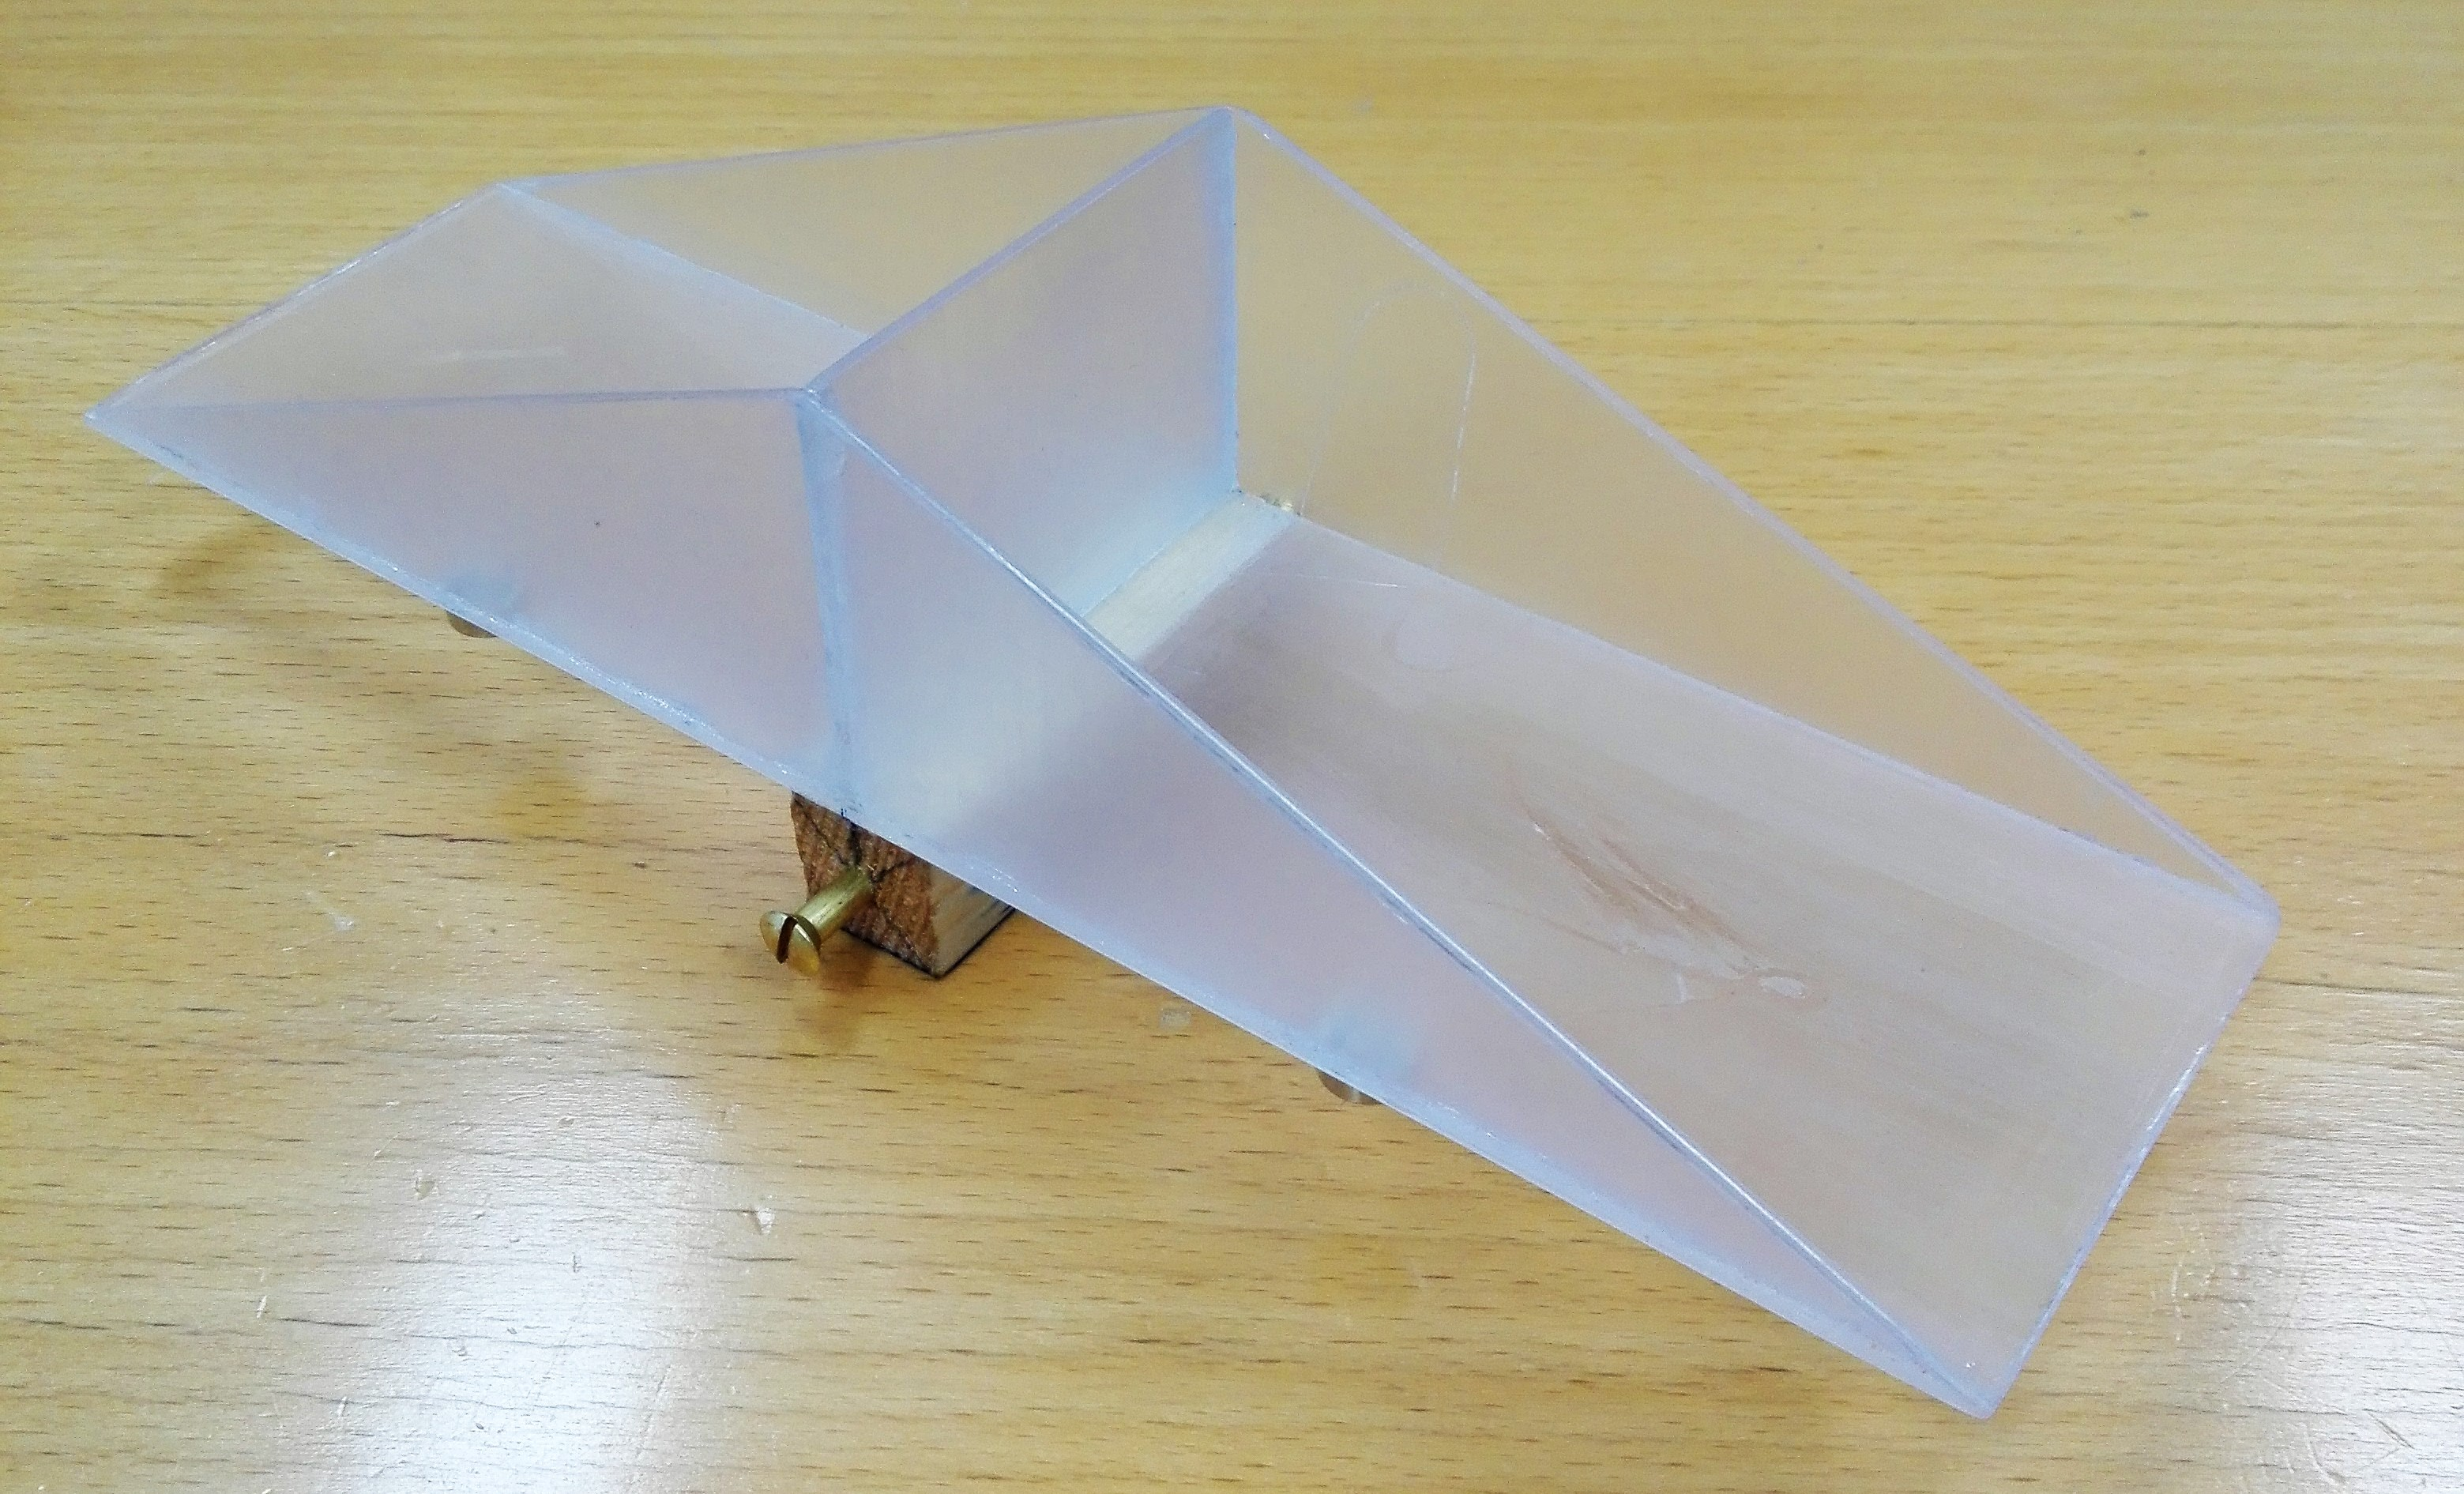
\includegraphics[width=0.8\linewidth]{graphics/Etappe1.jpg}
\caption{Selbsterstellter Kipplöffel.}
\label{fig:Etappe1}
\end{figure}

Abbildung \ref{fig:Etappe1} zeigt den selbsterstellten Kipplöffel aus Acrylglas. Die Drehachse ist mittig unter dem Kipplöffel befestigt und besteht aus einem Holzklotz mit je einer Schraube pro Seite.

\paragraph{\textbf{Etappe 2: Realisierung der drehbaren Lagerung}}
Die Drehbare Lagerung des Kipplöffels ist wichtig, damit der Kipplöffel auf beide Seiten kippen kann. Die Drehachse soll direkt unterhalb der Mitte des Kipplöffels befestigt sein um ein gleichmässiges Kippen zu ermöglichen. Die Höhe des Kipplöffels wird definiert durch die einstellbare Höhe der Drehachsenlagerung. 

Die Drehachse wird aus einem Stück Holz und zwei Schrauben gefertigt, wobei das Holz direkt am Kipplöffel befestigt wird. Die zwei Schrauben werden auf einem höhenverstellbarem Gerüst gelagert, so dass ein drehen möglich ist. Dieses Gerüst wird auch aus Holz gefertigt und enthält eine Metallische Fläche an der Kontaktstelle der zuvor erwähnten Schrauben, um aufkommende Reibkräfte zu verringern. Ausserdem ist dieses Gerüst höhenverstellbar über zwei mit Muttern feststellbaren Gewinden (für jede Seite eine). 

\begin{figure}[h]
\centering
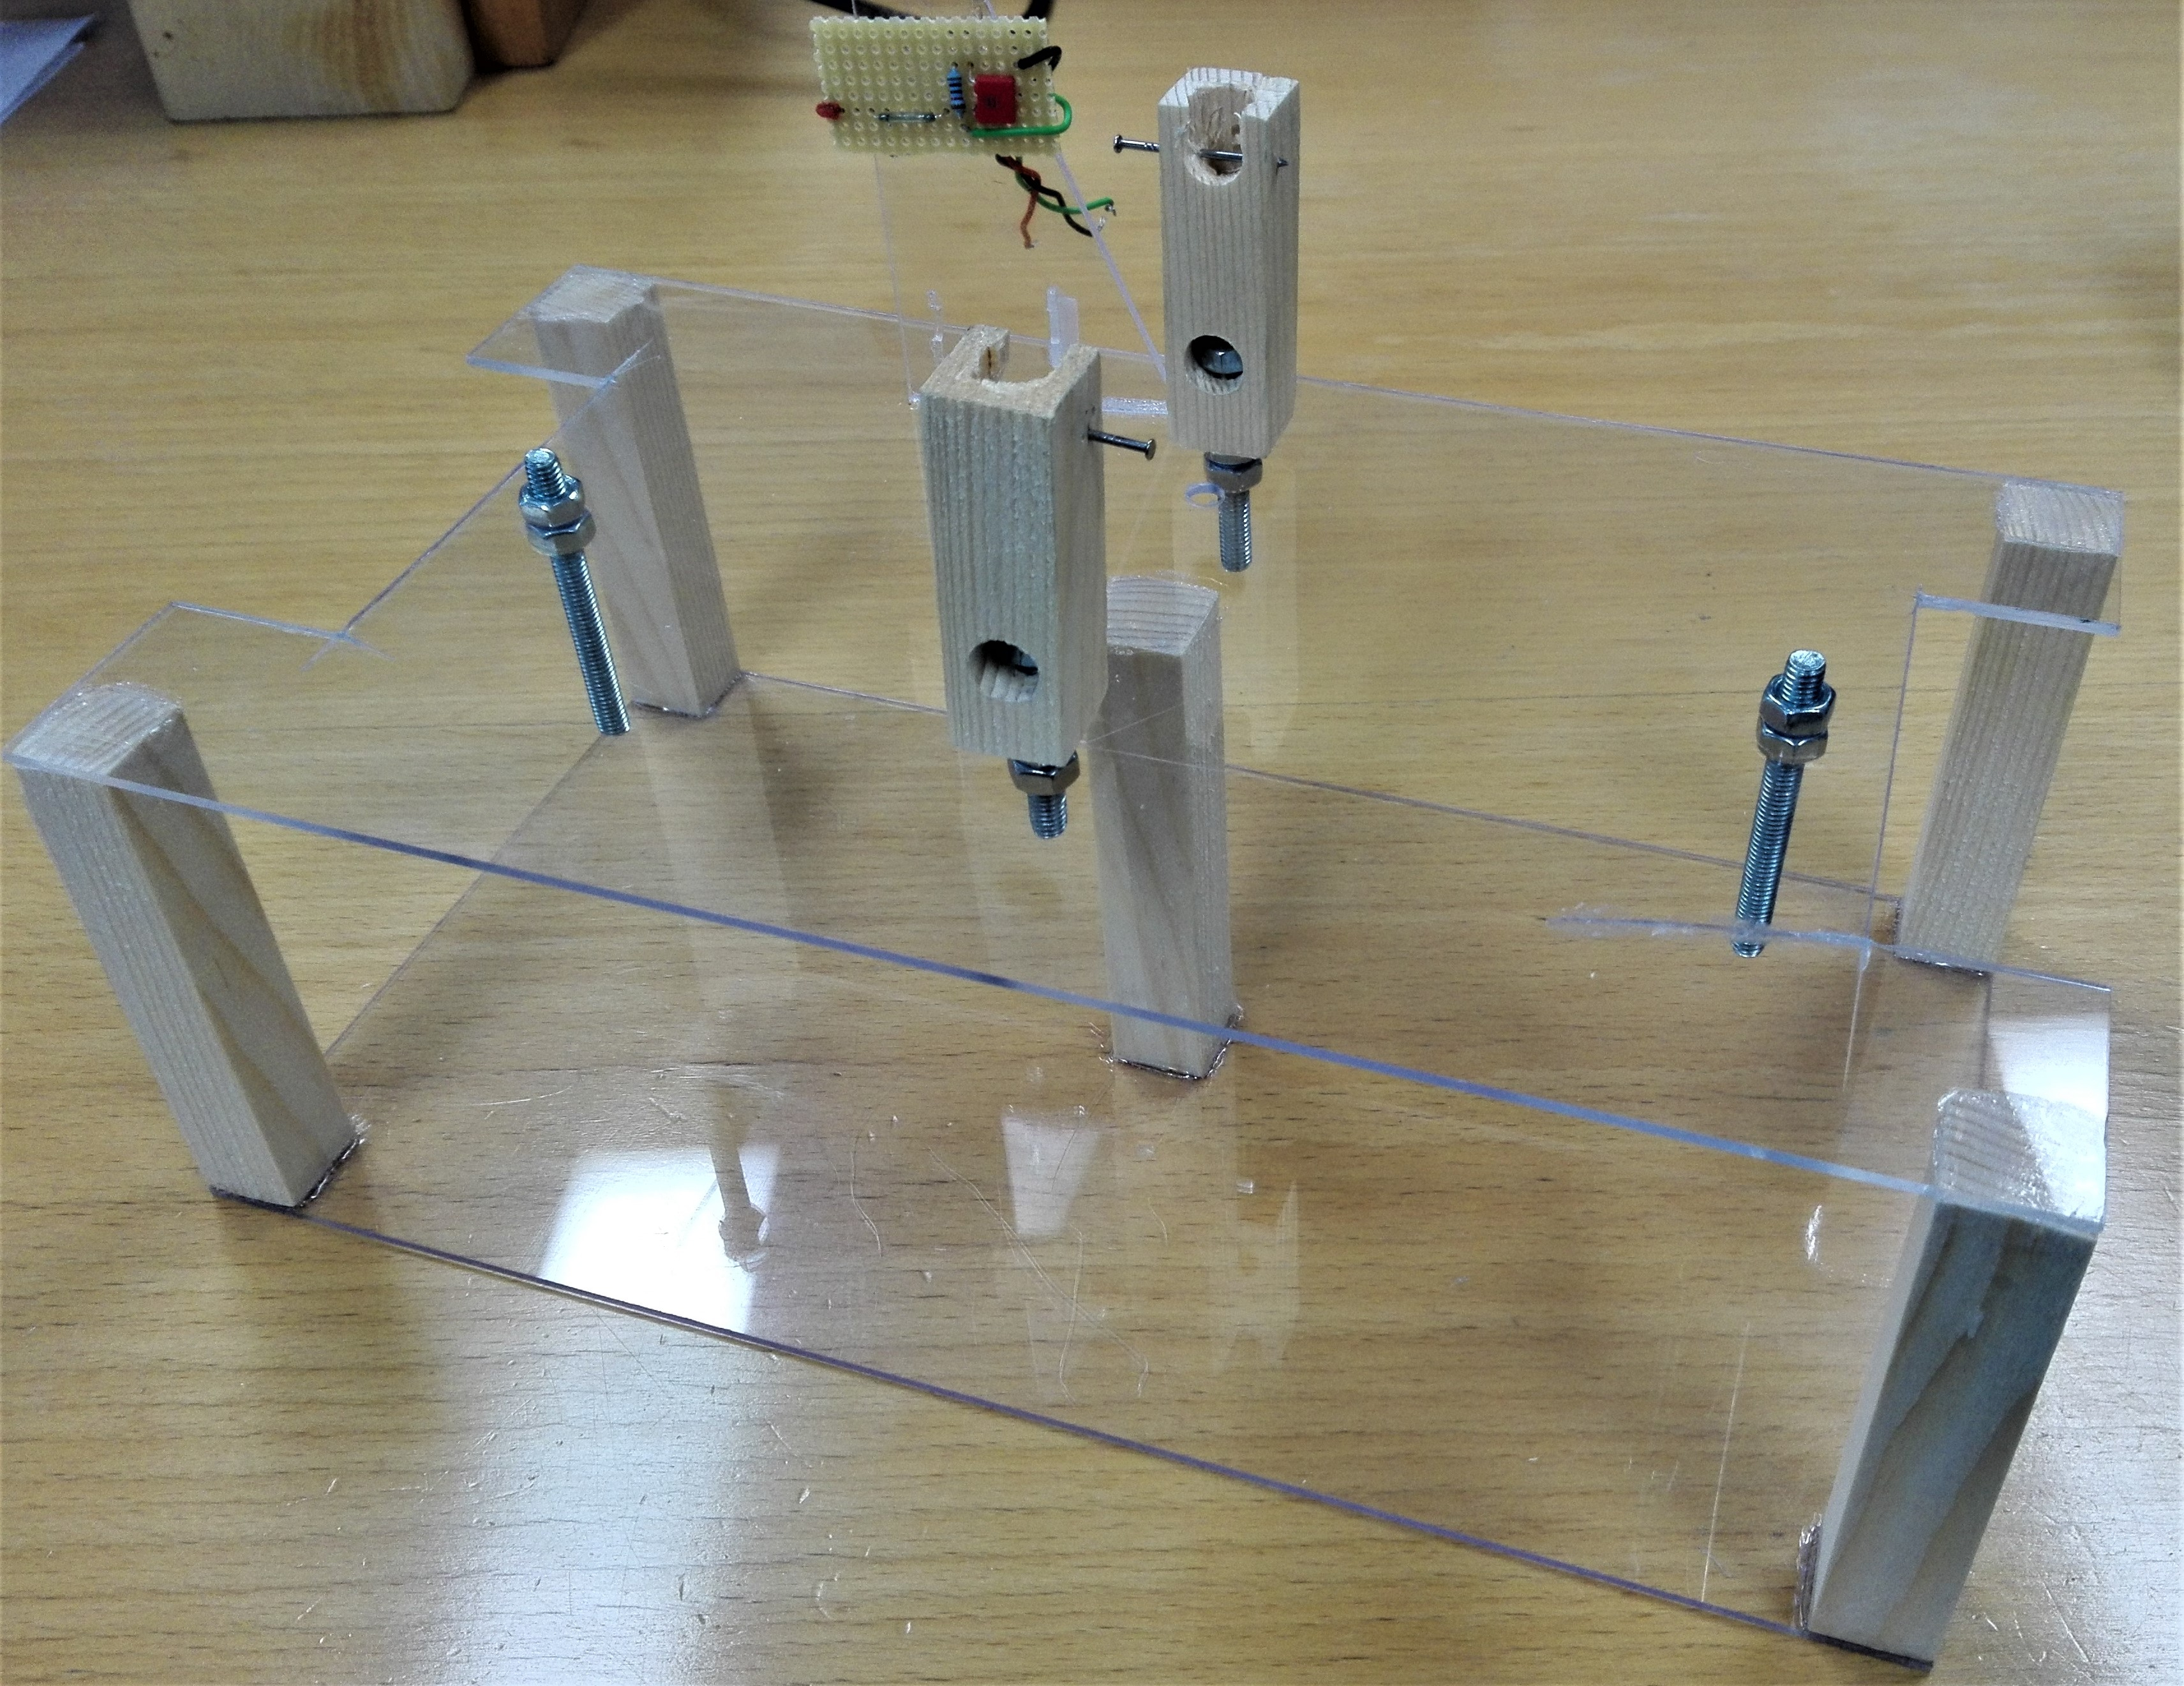
\includegraphics[width=0.8\linewidth]{graphics/Etappe2.jpg}
\caption{Selbsterstelltes Gerüst.}
\label{fig:Etappe2}
\end{figure}

Abbildung \ref{fig:Etappe2} zeigt das selbsterstellte Gerüst für die Höhenverstellbare, drehbare Lagerung des Kipplöffels. Es kann sowohl die Höhe des Kipplöffels, sowie dessen Neigung in den Endpositionen über Gewinden mit Muttern eingestellt werden. Die Schrauben des Kipplöffels kommen auf einen Stahlnagel zu liegen, womit Reibungsverluste gering gehalten werden.

\paragraph{\textbf{Etappe 3: Realisierung des Trichters}}
Der Trichter sorgt dafür, dass der Regen, welcher auf die Trichterfläche fällt, über der Mitte des Kipplöffels in den Löffel fliesst. Die Trichterfläche stellt gleichzeitig die Referenzfläche dar, da die gesamte Regenmenge dieser Fläche über den Kipplöffel erfasst wird. Ist diese Fläche von 1 $m^2$ abweichend, so muss in der Firmware ein Skalierungsfaktor implementiert werden, damit die Regenmenge wie gewünscht gemäss Pflichtenheft ermittelt werden kann. Der Trichter wird aus demselben Material gefertigt wie der Kipplöffel, da hier die gleichen Anforderungen gelten. Es sei angemerkt, dass der Trichter nur bei weiteren Verwendung des selbst erstellten Kipplöffels, zusammen mit dem Gehäuse der gesamten Wetterstation, erstellt wird.

\paragraph{\textbf{Etappe 4: Realisierung des Gehäuses}}
Das Gehäuse soll den Sensor vor ungewollten äusseren Einflüssen schützen, sowie umgebende Elektronik vor eventuellen Regenwasserspritzer. Ausserdem soll ein Schaltkreis mit Reedrelais implementiert werden, damit die Kippbewegungen von der Elektronik erfasst werden können. Es sei erwähnt, dass das Gehäuse nur bei weiteren Verwendung des selbst erstellten Sensors, zusammen mit dem Gehäuse der Wetterstation, konstruiert wird.

\paragraph{\textbf{Implementierung des Schaltkreises}}
Der Schaltkreis, welcher die Kippbewegungen feststellen soll, besteht im wesentlichen aus einem Reedrelais und einem Permanentmagneten. Das Reedrelais ist NO (Normally Open) und wirkt als stromkreisschliessender Schalter, sobald ein magnetisches Feld (z.B. das eines Permanentmagneten) sich in unmittelbarer Nähe befindet. Der Permanentmagnet wird auf dem Kipplöffel befestigt und das Reedrelais als Gegenstück an einem Fixpunkt in der Nähe. Wichtig dabei ist, dass das Reedrelais bei den Endpositionen des Kipplöffels nicht geschlossen ist, damit der Stromkreis geöffnet ist und Strom gespart werden kann. Das Reedrelais benötigt einen seriellen Widerstand, damit bei einem schliessen des Stromkreises kein Kurzschluss auftritt. Ausserdem soll ein Kondensator parallel zum Widerstand sein, um die Speisespannung zu glätten und so ein nutzbares Signal zu erhalten. Die Speisespannung stellt den Pegel für ein schliessen des Reedrelais, und somit auch für eine Kippbewegung dar. Um die Kippbewegungen zu zählen, kann somit entweder jede steigende oder jede fallende Flanke des Signals gezählt werden.  

\begin{figure}[h]
\centering
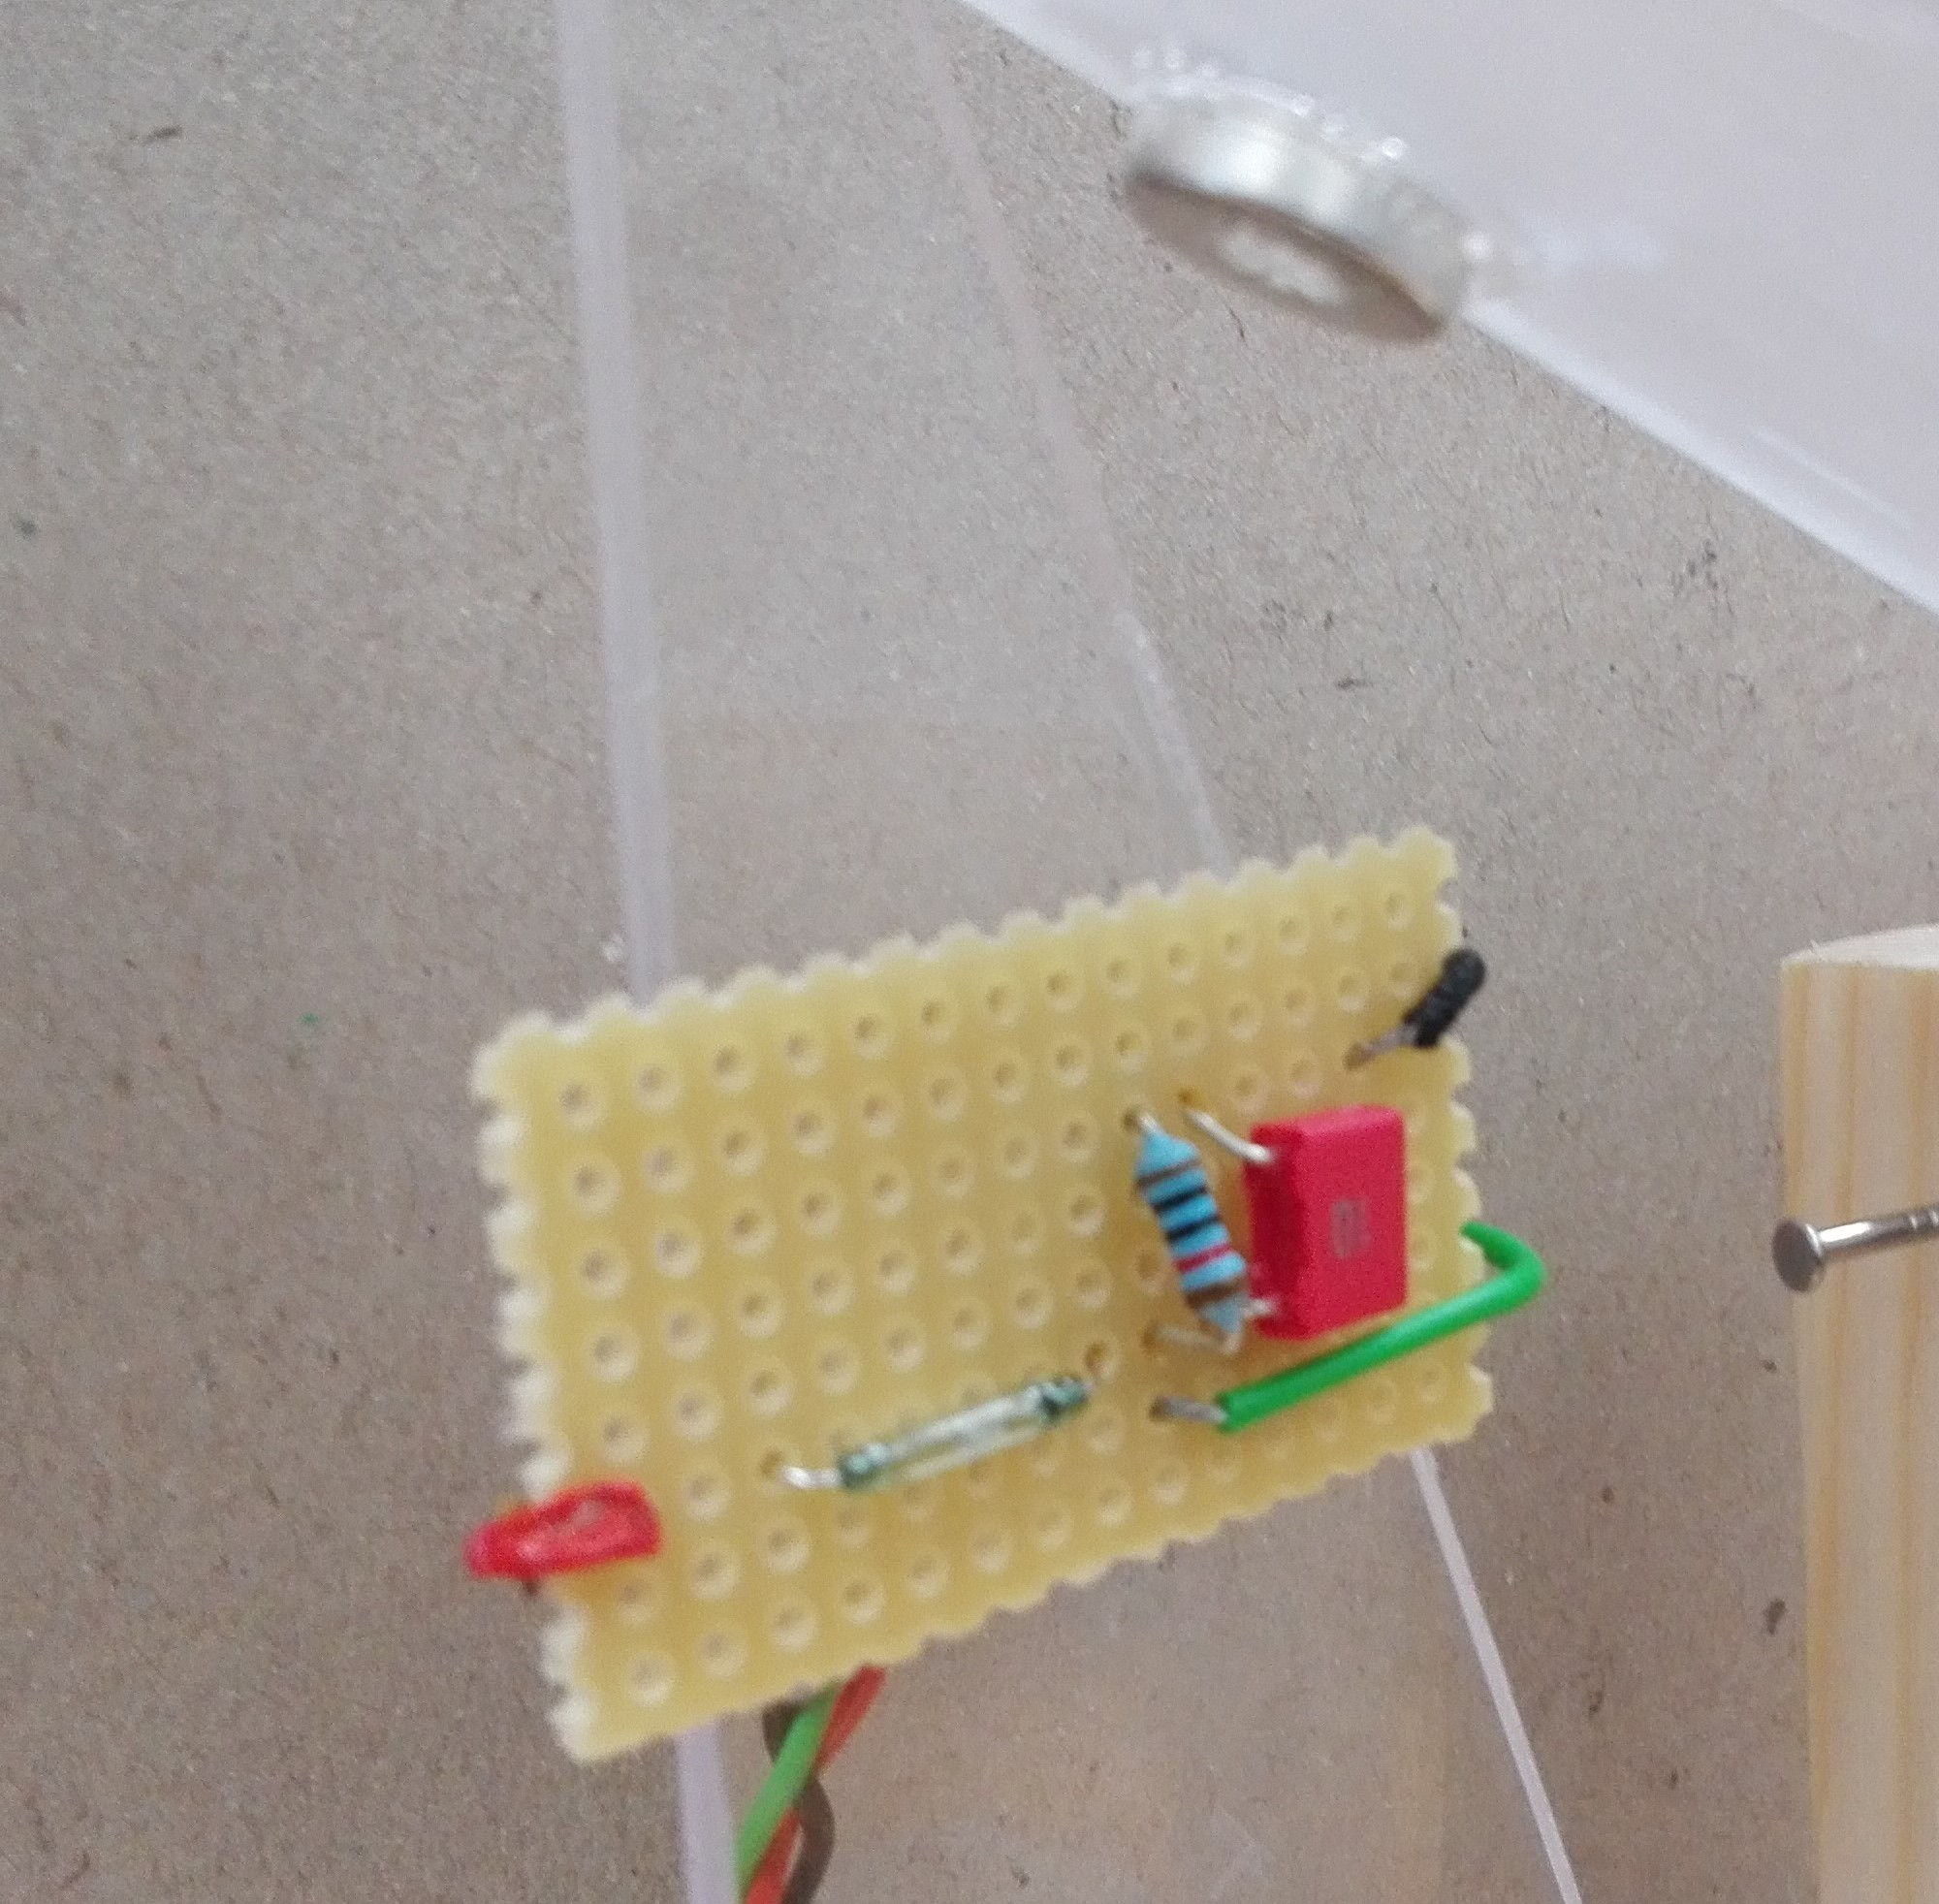
\includegraphics[width=0.35\linewidth]{graphics/KippSchalt.jpg}
\caption{Schaltkreis zur detektion der Kippbewegung.}
\label{fig:KippSchalt}
\end{figure}

Abbildung \ref{fig:KippSchalt} zeigt den Schaltkreis zur detektion der Kippbewegung. Benutzt wurde ein 10k$\Omega$ Widerstand mit einem parallel angeschlossenen 100nF Kondensator. Der Reedkontakt reagiert auf den ebenso sichtbaren Permanentmagneten, welcher an der Unterseite des Kipplöffels befestigt ist.
\newpage
\paragraph{\textbf{Nachteile des Selbstgebauten Niederschlagsmengensensor}}
Der selbstgebaute Niederschlagssensor beweist, dass das Prinzip des Kipplöffels funktioniert. Dennoch weist der Selbstbau Mängel auf. Der verwendete Permanentmagnet muss geklebt werden, weshalb dessen Magnetfeld massiv an stärke verliert und die Schaltung deshalb äusserst nahe angebracht werden muss. Ausserdem kam es, dadurch dass keine Werkstatt zugänglich war, zu Improvisation bei nahezu allen Fertigungsschritten, was zu unkalkulierbaren Abweichungen führt. Als Beispiel sei das Spiel der drehbaren Lagerung des Kipplöffels auf dem Gerüst angeführt, was jegliche Justierungsversuche der Niederschlagsmenge beeinflusst. Aus den genannten Gründen wird vorgefertigter Sensor mit Kipplöffelprinzip verwendet.

\begin{figure}[hbtp]
\centering
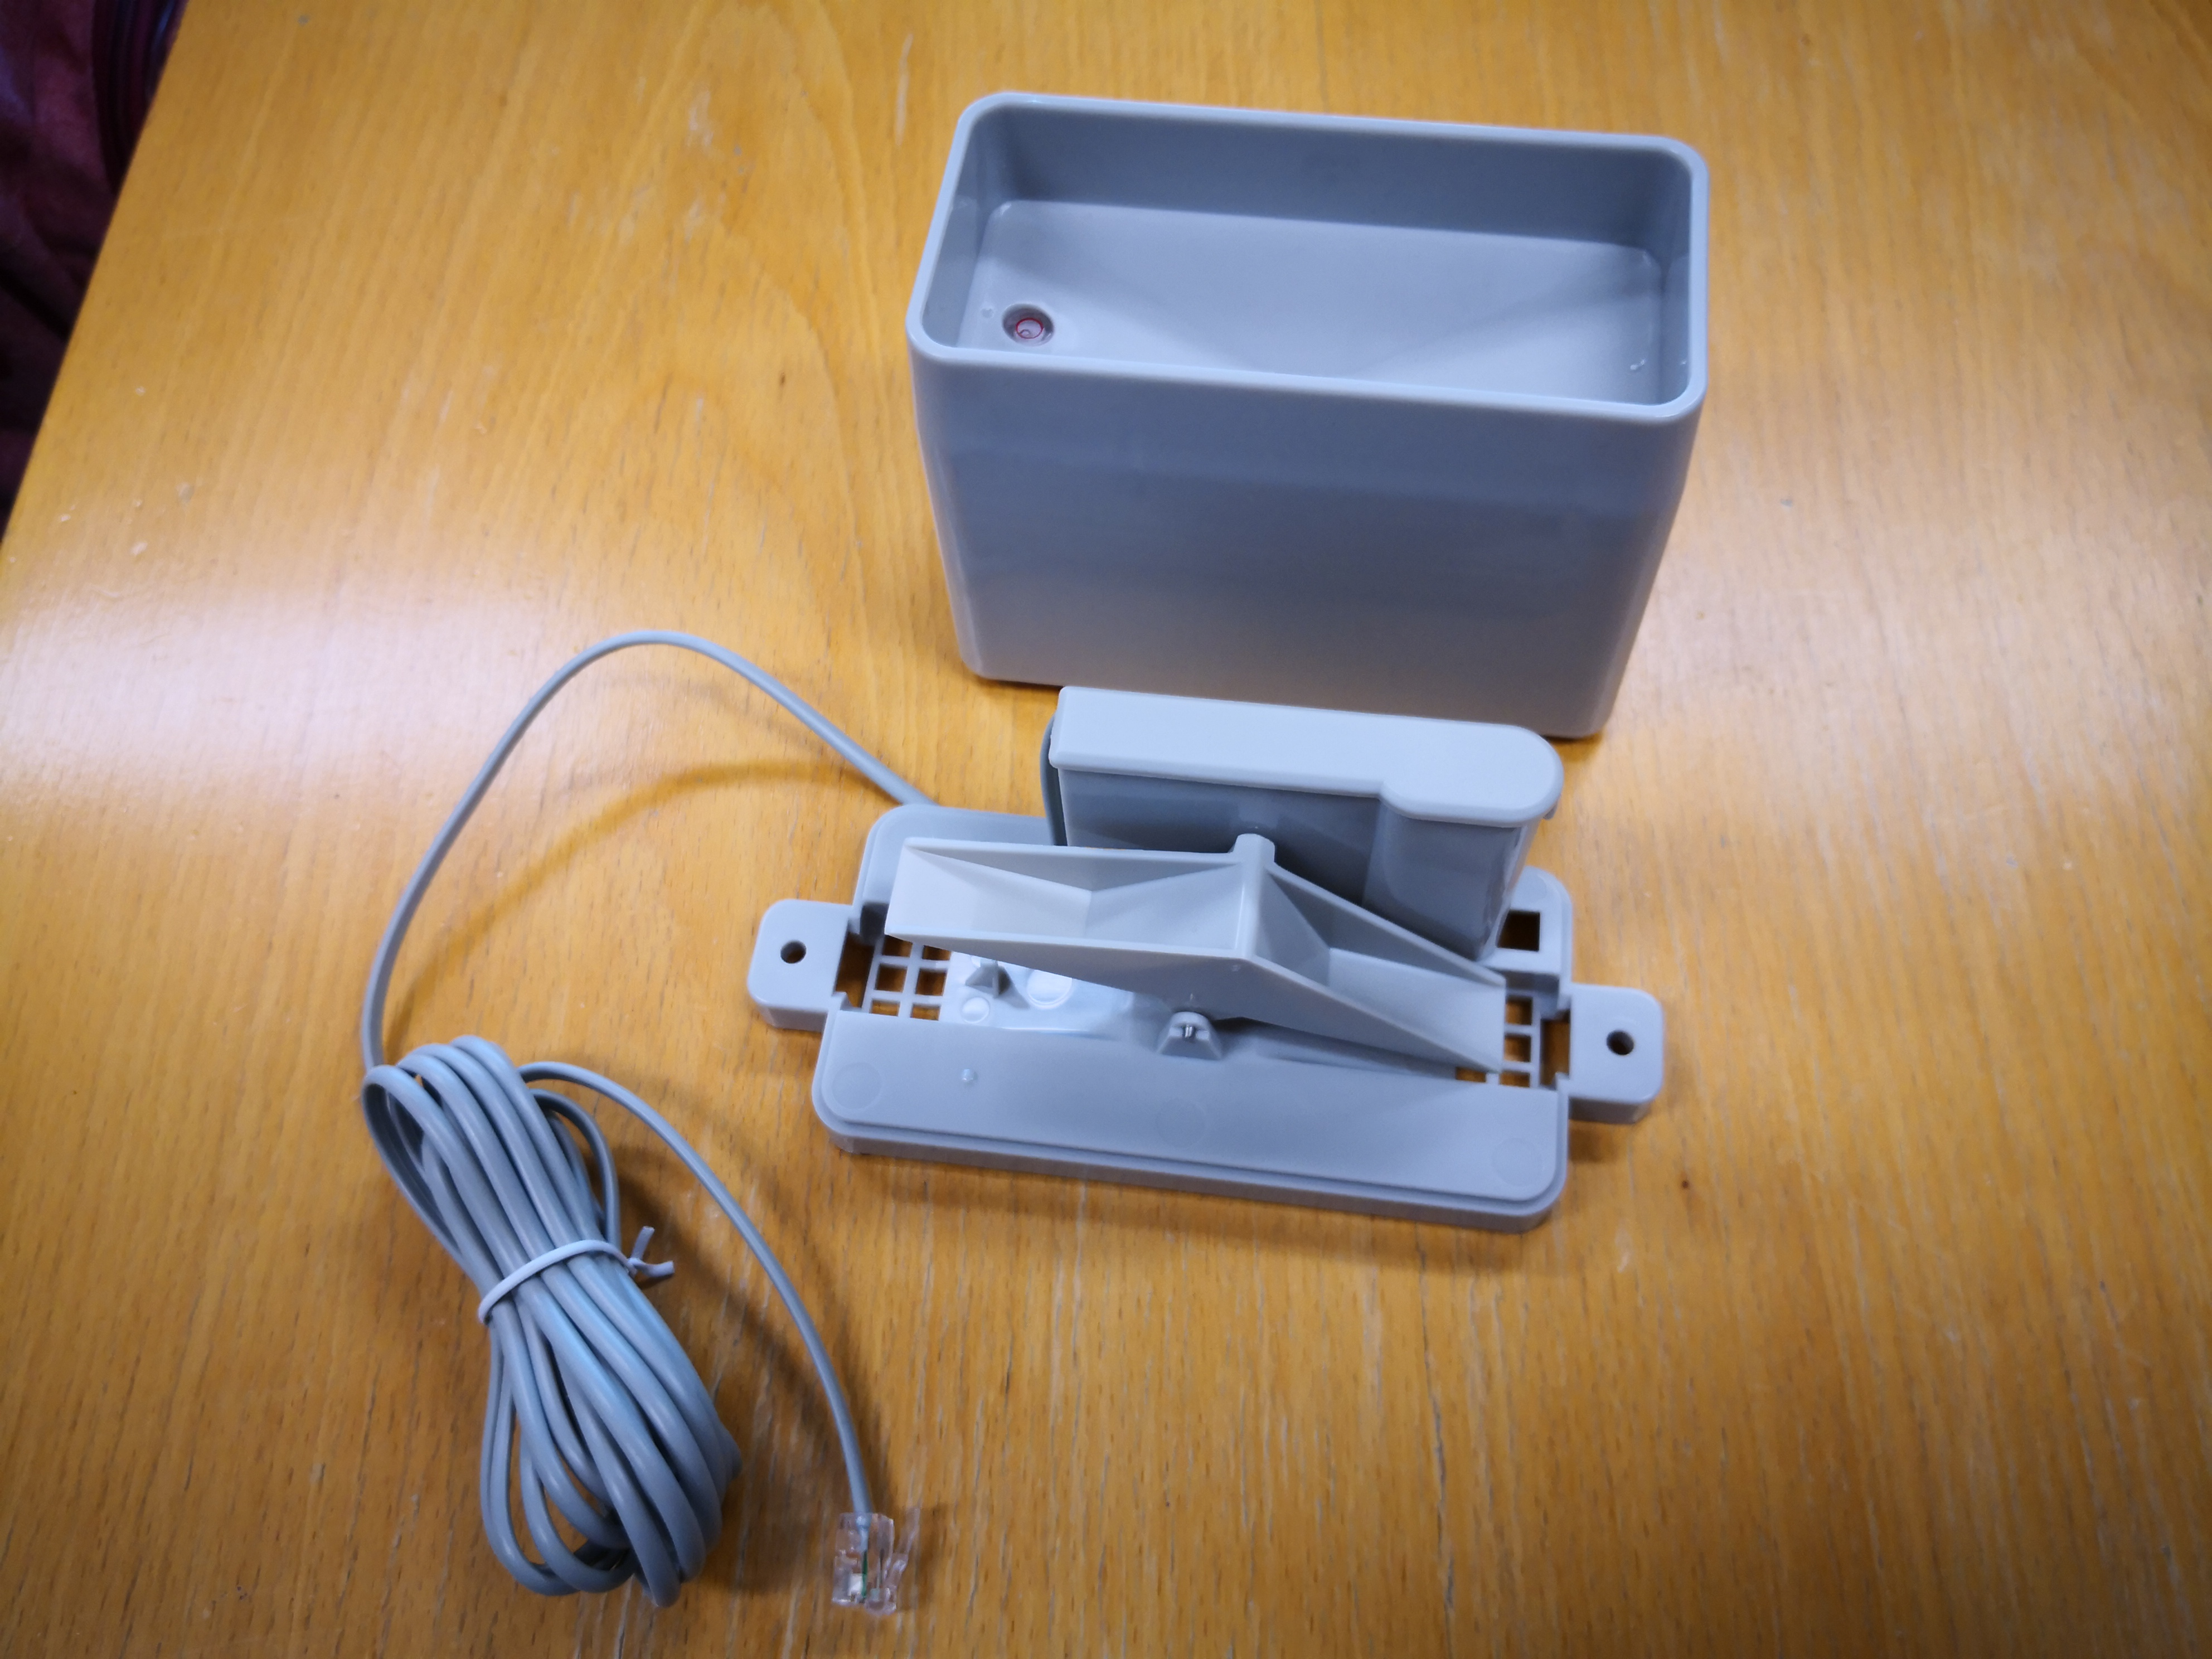
\includegraphics[width=0.7\textwidth]{graphics/ombrometer/IMG_20190118_110027.jpg}
\caption{Das Ombrometer}
\label{fig:verwendetes_ombrometer}
\end{figure}

Das verwendete Ombrometer von MISOL hat eine Auflösung von ca. 2ml pro Kippbewegung auf auf die Dimensionen $5.5E-2m*11.5E-2m$ des Trichters. Zudem enthält der Trichter oben noch eine kleine Wasserwaage, damit das Ombrometer auch gerade steht und die gemessene Regenmenge nicht verfälscht wird.

%\subsubsection*{Implentation in der Firmware}
%Die Implementation wurde über einen Interrupt-Pin des ATMega2560 gemacht. Jedes mal wenn der Kipplöffel des Ombrometers kippt, wird ein Interrupt der auf die steigende Flanke des anliegenden Signals getriggert ist ausgeführt, welcher einen Counter für das Ombrometer inkrementiert. Eine Kippbewegung des Ombrometers umfasst ca. 2ml auf eine Fläche von $5.5E-2m*11.5E-2m=\underline{\underline{6.325E-3m^{2}}}$. Hochgerechnet auf einen Quadratmeter ergibt sich
%\begin{equation}
%2ml*\dfrac{1m^{2}}{6.325E-3m^{2}} = \underline{\underline{316.21ml}}
%\end{equation}
%benötigter Niederschlag für eine Kippbewegung des Ombrometers pro Quadratmeter. Nun kann die Niederschlagmenge in einem bestimmten Zeitraum ausgegeben werden.\\

\subsubsection{Anemometer}
{\begin{minipage}[b][650pt][t]{0.55\textwidth}
Für die Windgeschwindigkeitsmessung wurde ein Ersatz Anemometer von Froggit genommen (Abb. \ref{fig:anemometer}). Das Anschlusskabel hat einen vier poligen RJ-11 Stecker, dessen Signal über eine Buchse zum MCU geführt wird. Das Anemometer selbst hat allerdings nur zwei Anschlüsse, die Speisung (rot) und das durch einen mit einem Dauermagneten schließbaren Reedkontakt modulierte pulsförmige Ausgangssignal (grün, Abb. \ref{fig:rj11stecker}). In der Abb. \ref{fig:beschaltungAnemometer} ist ersichtlich, dass das Ausgangssignal über R1 abfällt und C1 als Spannungsstabilisierung dient. Das daraus resultierende Signal ist in der Abb. \ref{fig:rechteckpuls_anemometer} aufgezeigt. Die Windgeschwindigkeit ist nun aus der Anzahl Rechteckpulsen direkt interpretierbar:\\

Wenn über einen Zeitraum $T$ die Anzahl Pulse $A$ gemessen werden, dann kann auf die Winkelgeschwindigkeit $\omega$ nach 
\begin{equation}
\centering
\omega=\frac{A}{T}\qquad[s^{-1}]
\end{equation}
geschlossen werden. Da allerdings verschiedene Faktoren wie das Trägheitsmoment des Schalenkreuzes, Reibungsverluste bei der Drehbewegung, Verfälschung bei wechselnder Windrichtung usw. zusätzlich auf das Anemometer wirken, wird es sehr komplex die Windgeschwindigkeit exakt zu berechnen. Deshalb wird nur ein Näherungswert ermittelt und mit einem Skalierungsfaktor $SF$ korrigiert. Somit ergibt sich für die Windgeschwindigkeit $v_{Wind}$ mit Radius $r$ des Schalenkreuzes
\begin{equation}
\centering
v_{Wind} = \frac{A\cdot r\cdot SF}{T}\qquad[m/s].
\label{equ:berechnungWindgeschwindigkeit}
\end{equation}
Der Skalierungsfaktor $SF$ wird mittels Referenzmessungen der Windgeschwindigkeit eines digitalen Anemometers eruiert. \\
\end{minipage}}
{\begin{minipage}[b][650pt][t]{0.44\textwidth}
\centering
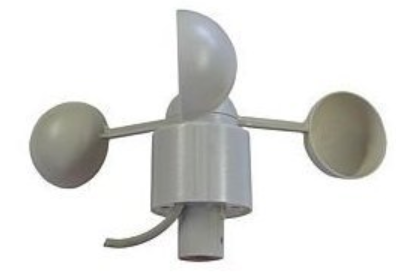
\includegraphics[width=0.9\textwidth]{graphics/Anemometer/anemometer.png}
\captionof{figure}{Anemometer \cite{AmazonAnemometer}}
\label{fig:anemometer}
\vspace{20pt}
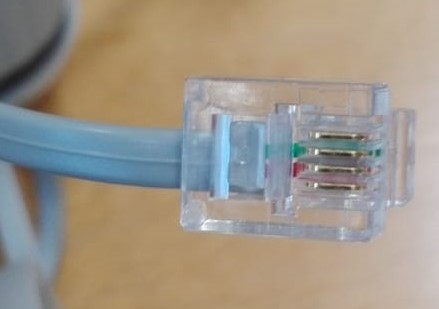
\includegraphics[width=0.9\textwidth]{graphics/Anemometer/rj_11_anschlussstecker.png}
\captionof{figure}{RJ-11 Stecker}
\label{fig:rj11stecker}
\vspace{20pt}
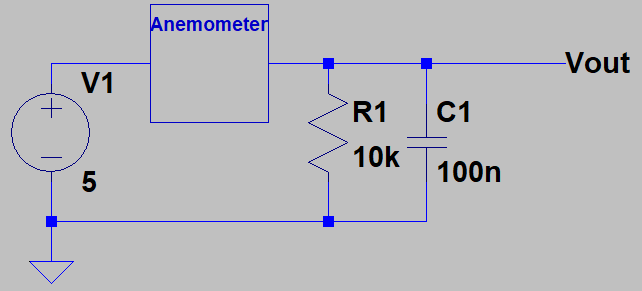
\includegraphics[width=0.9\textwidth]{graphics/Anemometer/schaltung_anemometer.png}
\captionof{figure}{Beschaltung des Ausgangs des Anemometers.}
\label{fig:beschaltungAnemometer}
\vspace{20pt}
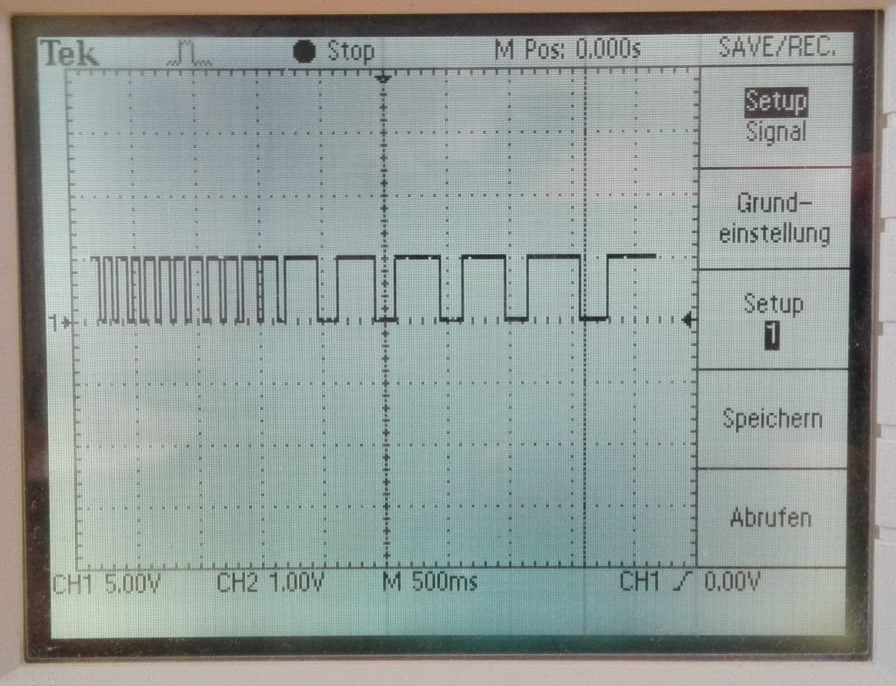
\includegraphics[width = 0.9\textwidth]{graphics/Anemometer/oszilloskop_anenometer_puls.png}
\captionof{figure}{Ausgangssignal $V_{out}$}
\label{fig:rechteckpuls_anemometer}
\end{minipage}}
\newpage

%\subsubsection*{Implementation in die Firmware}
%Die Implementation wurde recht simpel gehalten. Der gesamte implementierte Code für das Anemometer ist im Headerfile ''Anemometer.h'' extern deklariert und im File Anemometer.cpp initialisiert. Das Signal $V_{out}$ ist mit einen digital Pin des Atmega 2560 (Pinnummer 2 des Arduino Mega Boards) verbunden. Über einen Zeitraum von $5000ms$, auf die steigende Flanke getriggert, wird die Anzahl von Pulsen mittels Interrupt\footnote{es handelt sich hierbei um \textit{external Interrupts}.} gezählt. Dabei wird zuerst der Interrupt auf der Pinnummer 2 aktiviert, mit einem Delay von $5000ms$ gewartet, wobei bei jedem ausgelösten Interrupt die Funktion \textcolor{orange}{countWind}() ausgeführt und somit bei jeder steigenden Flanke um eins inkrementiert wird. Zum Schluss folgt die Deaktivierung des Interrupts und die Berechnung der Windgeschwindigkeit nach der Gleichung \ref{equ:berechnungWindgeschwindigkeit}.\\

\subsubsection{Windrichtungsgeber}
{\begin{minipage}[b][10cm][t]{0.55\textwidth}
Um die Windrichtung angeben zu können, wurde ein Windrichtungsgeber, wie in Abb. \ref{fig:windrichtungsgeber} gezeigt von MISOL verwendet. Er ist genau wie das Ombrometer und das Anemometer mit Reedkontakten realisiert worden (siehe Abb. \ref{fig:interne_schaltung}). Dafür sind acht Reedkontakte im Kreis angeordnet und jeder hat einen in Serie geschalteten Widerstand von unterschiedlichen Dimensionen. Der Dauermagnet kann, je nach Drehwinkel bis zu zwei Reedkontakte gleichzeitig schließen. Dies erlaubt sechzehn verschiedene Winkelpositionen und somit eine Auflösung von 22.5$^{o}$. Mit einem externen Widerstand $R=10k\Omega$ (siehe Abb. \ref{fig:aussere_beschaltung}) wird eine Spannung generiert, welche dann mit dem ADC des Microcontrollers gelesen werden kann. Der Windrichtungsgeber wird mit einer Speisespannung von $V_{+}=5V$ betrieben. Der Windrichtungsgeber hat einen vierpoligen RJ-11 Anschluss. Zudem hat er auf der unteren Seite noch eine RJ-11 Buchse, bei der das Anemometer direkt angeschlossen werden kann. Wie diese Anschlüsse gemapped sind, wird in der Abb. \ref{fig:interne_schaltung} gezeigt. \\
\end{minipage}}
{\begin{minipage}[b][10cm][t]{0.44\textwidth}
\centering
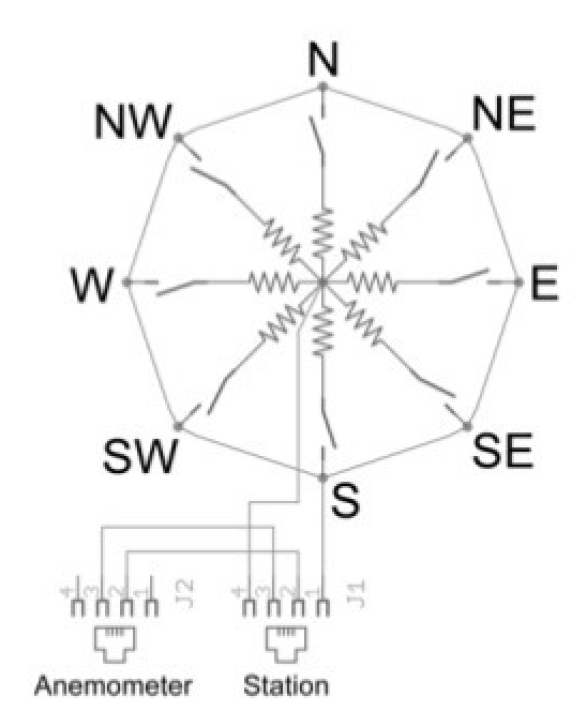
\includegraphics[width=0.9\textwidth]{graphics/windrichtungsgeber/interne_schaltung.PNG}
\captionof{figure}{Interne Schaltung \cite{ADSkeineAngabe}}
\label{fig:interne_schaltung}
\end{minipage}}

\begin{table}[h]
\centering
\caption{Technische Werte \cite{ADSkeineAngabe}}
\begin{tabular}{|c|c|c|c|}
\hline 
Richtung [$^{o}$] & Himmelsrichtung & Widerstand [$\Omega$] & Ausgangsspannung [V] \\ 
\hline 
0 & N & 33k & 3.84 \\ 
\hline 
22.5 &  & 6.57k & 1.98 \\ 
\hline 
45 & NE & 8.2k & 2.25 \\ 
\hline 
67.5 &  & 891 & 0.41 \\ 
\hline 
90 & E & 1k & 0.45 \\ 
\hline 
112.5 &  & 688 & 0.32 \\ 
\hline 
135 & SE & 2.2k & 0.90 \\ 
\hline 
157.5 &  & 1.41k & 0.62 \\ 
\hline 
180 & S & 3.9k & 1.40 \\ 
\hline 
202.5 &  & 3.14k & 1.19 \\ 
\hline 
225 & SW & 16k & 3.08 \\ 
\hline 
247.5 &  & 14.12k & 2.93 \\ 
\hline 
270 & W & 120k & 4.62 \\ 
\hline 
292.5 &  & 42.12k & 4.04 \\ 
\hline 
315 & NW & 64.9k & 4.33 \\ 
\hline 
337.5 &  & 21.88k & 3.43 \\ 
\hline 
\end{tabular} 
\label{tab:technische_werte}
\end{table}

In der Tabelle \ref{tab:technische_werte} sind die Widerstandswerte der in Abb. \ref{fig:interne_schaltung} gezeigten Widerständen und die Werte der Ausgangsspannung bei variabler Winkelposition aufgelistet. Da nun abhängig von der Winkelposition unterschiedliche Widerstände parallel geschalten werden, resultiert am Ausgang eine vom Winkel abhängige Ausgangsspannung.\\

\newpage


{\begin{minipage}[b][6cm][t]{0.49\textwidth}
\centering
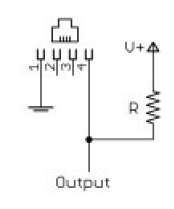
\includegraphics[width=0.5\textwidth]{graphics/windrichtungsgeber/aeussere_beschaltung.PNG} 
\captionof{figure}{Spannungsteiler mit $R=10k\Omega$ \cite{ADSkeineAngabe}}
\label{fig:aussere_beschaltung}
\end{minipage}}
{\begin{minipage}[b][6cm][t]{0.49\textwidth}
\centering
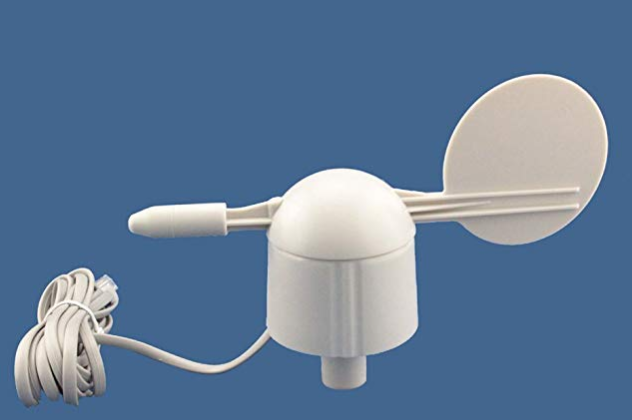
\includegraphics[width=0.9\textwidth]{graphics/windrichtungsgeber/windrichtungsgeber.PNG}
\captionof{figure}{Windrichtungsgeber von MISOL \cite{windrichtungsgeber}}
\label{fig:windrichtungsgeber}
\end{minipage}}

%\subsubsection*{Implementation in die Firmware}
%Der ADC hat des ATMega2560 hat eine 10 Bit Auflösung und wird mit 5 Volt betrieben. Um das Signal am ADC lesen zu können, wird die Funktion \textit{analogRead()} aufgerufen. Als Rückgabewert wird ein binärer Wert als Dezimalzahl vom Datentyp \textit{float} erhalten. Um diesen Wert in die eigentlich am ADC anliegende Spannung umzurechnen wird die Gleichung \ref{equ:ADC1} umgeformt.
%\begin{equation}
%\centering
%\dfrac{Auflösung ADC}{Betriebsspannung} = \dfrac{analogRead()}{Ausgangsspannung}
%\label{equ:ADC1}
%\end{equation}
%Daraus resultiert:
%\begin{equation}
%\centering
%Ausgangsspannung = \dfrac{analogRead()*Betriebsspannung}{Auflösung ADC}
%\label{equ:ADC2}
%\end{equation}
%Werden nun die Werte in die Gleichung \ref{equ:ADC2} eingefügt, ergibt sich für die Ausgangsspannung $V_{out}$:
%\begin{equation}
%\centering
%V_{out}(analogRead()) = \dfrac{analogRead()*5V}{10}
%\label{equ:adc_vout}
%\end{equation}
%Diese von \textit{analogRead()} abhängige Ausgangsspannung $V_{out}$ wird dann in \textit{if else} Anweisungen zu der Himmelsrichtung zugewiesen und als String abgespeichert.

\subsubsection{BME280}
\label{BME280}
{\begin{minipage}[b][6cm][t]{0.55\textwidth}
Der \textit{BME280} ist ein low powered digitaler Feuchtigkeits-, Luftdruck- und Temperatursensor von Bosch. Er ist in einem 2.5mm x 2.5mm x 0.93mm metal lid LGA Gehäuse verpackt und kann über die Interfaces I$^{2}$C und SPI kommunizieren. Durch seinen niedrigen Stromverbrauch, große operating range der drei Messgrößen und schnellen Ansprechzeit von etwa 1s eignet er sich für die solarbetriebene mobile Wetterstation besonders. \cite{Bosch2019}\\
\end{minipage}}
{\begin{minipage}[b][6cm][t]{0.44\textwidth}
\centering
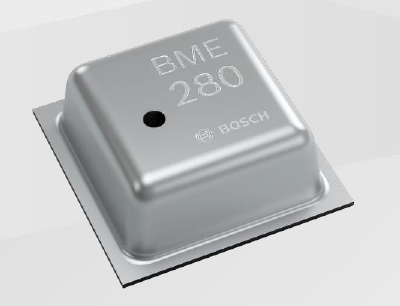
\includegraphics[width=0.9\textwidth]{graphics/bme280/bme280.PNG}
\captionof{figure}{BME280 \cite{Bosch2019}}
\label{fig:bme280}
%\vspace*{0.5cm}
%\centering
%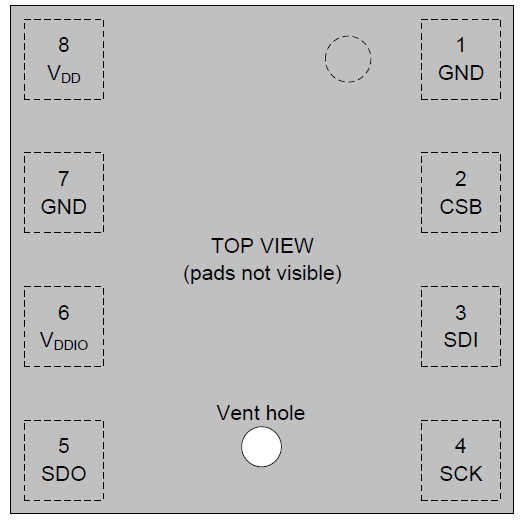
\includegraphics[width=0.9\textwidth]{graphics/bme280/bme280_pinout.PNG}
%\captionof{figure}{Pinout \cite{Bosch2019}}
%\label{fig:bme280_pinout}
\end{minipage}}

\begin{table}[h]
  \centering
  \caption{Elektrische Spezifikationen \cite{Bosch2019}}
    \begin{tabular}{lllll}
    \toprule
    \textbf{Parameter} & \textbf{Min.} & \textbf{Typ.} & \textbf{Max.} & \textbf{Einheit} \\
    \midrule
    Versorgungsspannung & 1.71  & 1.8   & 3.6   & V \\
    Stromverbrauch (sleep mode) &       & 0.1   & 0.3   & $\mu$A \\
    Stromverbrauch inaktiv (normal mode) &       & 0.2   & 0.5   & $\mu$A \\
    Stromverbrauch Feuchtigkeitsmessung &       & 340   &       & $\mu$A \\
    Stromverbrauch Luftdruckmessung &       & 714   &       & $\mu$A \\
    Stromverbrauch Temperaturmessung &       & 350   &       & $\mu$A \\
    \bottomrule
    \end{tabular}%
  \label{tab:elektrische_Spezifikationen}%
\end{table}%

Bei einer Messfrequenz von 1Hz für die drei Messgrößen verbraucht der BME280 somit laut Datenblatt nur \textbf{3.6$\mu$A}. \cite[S. 2]{Bosch2019}

\subsubsection*{\textbf{Feuchtigkeitsmessung}}
In der Tabelle \ref{tab:spez_feuchtigkeit} sind die wichtigsten Parameter zur Feuchtigkeitsmessung aufgelistet. Zu vermerken ist, dass die digitalen Werte des BME280 zur Feuchtigkeitsmessung relativ sind und deshalb prozentual angegeben werden. \\
\begin{table}[htbp]
  \centering
  \caption{Sezifikationen der Feuchtigkeitsmessung \cite{Bosch2019}}
    \begin{tabular}{lllll}
    \toprule
     \textbf{Parameter} & \textbf{Min.} & \textbf{Typ.} & \textbf{Max.} & \textbf{Einheit} \\
    \midrule
    Operating range & -40   & 25    & 85    & $^{o}$C \\
          & 0     &       & 100   & \% \\
    Absolute Genauigkeitstoleranz &       & $\pm$3 &       & \% \\
    Hysterese &       & $\pm$1 &       & \% \\
    Auflösung &       & 0.008 &       & \% \\
    Langzeitstabilität &       & 0.5   &       & \% pro Jahr \\
    \bottomrule
    \end{tabular}%
  \label{tab:spez_feuchtigkeit}%
\end{table}%

\newpage

\subsubsection*{\textbf{Luftdruckmessung}}
Die Genauigkeit der Luftdruckmessung ist an einen Temperaturbereich gebunden. Bei niedrigeren Temperaturen (<0$^{o}$C) weist der Sensor eine höhere Unsicherheit auf als bei Temperaturen von 0 bis 65 $^{o}$C (siehe Tabelle \ref{tab:spez_druck}). \\
\begin{table}[htbp]
  \centering
  \caption{Sezifikationen der Luftdruckmessung \cite{Bosch2019}}
    \begin{tabular}{llllll}
    \toprule
    \textbf{Parameter} & \multicolumn{1}{l}{\textbf{Temperaturbereich}} & \multicolumn{1}{l}{\textbf{Min.}} & \textbf{Typ. } & \multicolumn{1}{l}{\textbf{Max.}} & \textbf{Einheit} \\
    \midrule
    Operating range &       & \multicolumn{1}{l}{-40} & 25    & \multicolumn{1}{l}{85} & $^{o}$C \\
          &       & 300   &       & 1100  & hPa \\
    Absolute Genauigkeit & \multicolumn{1}{c}{-20 bis 0 $^{o}$C} &       & $\pm$1.7 &       & hPa \\
          & \multicolumn{1}{c}{0 bis 65 $^{o}$C} &       & $\pm$1  &       & hPa \\
    Auflösung &       &       & \multicolumn{1}{r}{0.18} &       & hPa \\
    Langzeitstabilität &       &       & $\pm$1  &       & hPa pro Jahr \\
    \bottomrule
    \end{tabular}%
  \label{tab:spez_druck}%
\end{table}%

\subsubsection*{\textbf{Temperaturmessung}}
Die Wetterstation wird hauptsächlich in einem Temperaturbereich von 0 bis 65 $^{o}$C betrieben, wodurch vom Sensor eine Unsicherheit von max. $\pm$1 $^{o}$C erreicht werden kann. \\
\begin{table}[htbp]
  \centering
  \caption{Sezifikationen der Temperaturmessung \cite{Bosch2019}}
    \begin{tabular}{llllll}
    \toprule
    \textbf{Parameter} & \multicolumn{1}{l}{\textbf{Temperaturbereich}} & \multicolumn{1}{l}{\textbf{Min.}} & \textbf{Typ. } & \multicolumn{1}{l}{\textbf{Max.}} & \textbf{Einheit} \\
    \midrule
    Operating range &       & \multicolumn{1}{l}{-40} & 25    & \multicolumn{1}{l}{85} & $^{o}$C \\
    Absolute Genauigkeit & \multicolumn{1}{c}{25 C} &       & $\pm$0.5 &       & $^{o}$C \\
          & \multicolumn{1}{c}{0 bis 65 C} &       & $\pm$1  &       & $^{o}$C \\
          & \multicolumn{1}{c}{-20 bis 0 C} &       & $\pm$1.25 &       & $^{o}$C \\
          & \multicolumn{1}{c}{-40 bis -20 C} &       & $\pm$1.5 &       & $^{o}$C \\
    Auflösung  &       &       & 0.01  &       & $^{o}$C \\
    \bottomrule
    \end{tabular}%
  \label{tab:spez_temp}%
\end{table}%

%\subsubsection*{Implementation in die Firmware}
%Um den BME280 vom Microcontroller aus ansteuern zu können, wurden zwei bereits existierende Librarys von Adafruit verwendet:
%\begin{itemize}
%\item Adafruit BME280 Library
%\item Adafruit Unified Sensors
%\end{itemize}
%Anschließend konnten die Headerfiles <Adafruit\_Sensor.h> und <Adafruit\_BME280.h> inkludiert werden und der Sensor über das I$^{2}$C Interface mit den folgenden Funktionen abgefragt werden:\\
%\begin{itemize}
%\item \textcolor{blue}{float} \textcolor{orange}{readTemperature}()
%\item \textcolor{blue}{float} \textcolor{orange}{readHumidity}()
%\item \textcolor{blue}{float} \textcolor{orange}{readPressure}()
%\end{itemize}

\subsection{Ergänzungen aus der Bachelor-Thesis}
Während der Bachelor-Thesis soll ein Sensor zur Ermittlung der Sonnenstunden implementiert werden. Um dies zu erreichen wurde die Idee, die Sonnenstunden direkt über den Ladestrom der Photovoltaikanlage zu eruieren, verworfen, da auf diese Weise mit höheren Energieverlusten zu rechnen wäre durch das Abzweigen des Ladestroms und die damit verbundene zusätzliche Speisung der zusätzlichen Schaltung. Stattdessen wird über ein Lichtintensitätssensor die Bestrahlungsstärke gemessen, womit die Sonnenstunden über einen Schwellwert berechnet werden können. Im folgenden Abschnitt wird der verwendete Lichtintensitätssensor näher erläutert.

\subsubsection{Lichtintensitätssensor}
Die Lichtintensität wird über den TSL2561, ein digitaler low power Sensor, eruiert. Dieser misst über eine Kombination aus einer Breitband-Photodiode und einer Infrarot-Photodiode die Lichtstärke mit einer 16-Bit Auflösung. Über zwei integrierte AD-Wandler wird der Photodiodenstrom gewandelt und auf einen digitalen Ausgang gegeben. Über eine I$^{2}$C Schnittstelle kann dieser Ausgang auf die MCU gegeben und so ausgewertet werden. Ab einem bestimmten Schwellenwert kann die Einstrahlung als direkte Sonnenstrahlung definiert, und so auch gezählt werden. Der erwähnte Schwellwert ist vom Ort abhängig an dem die Wetterstation sich befindet und muss eruiert und in der Firmware eingestellt werden, was im entsprechenden Teil (\refname{part:Firmware} \ref{part:Firmware})) erläutert wird. Da dieser Sensor nicht direkt auf der Platine sondern am oberen Teil des Gehäuses montiert werden muss, wird der TSL2561 als Breakout Board (Abbildung \ref{fig:TSL}) verwendet und über Pinheader mit dem PCB verbunden. Die wichtigsten elektrischen Spezifikationen sind in der Tabelle \ref{tab:TSL2561} zusammengefasst. \cite{TSL2561}\\

\begin{figure}[hbtp]
\centering
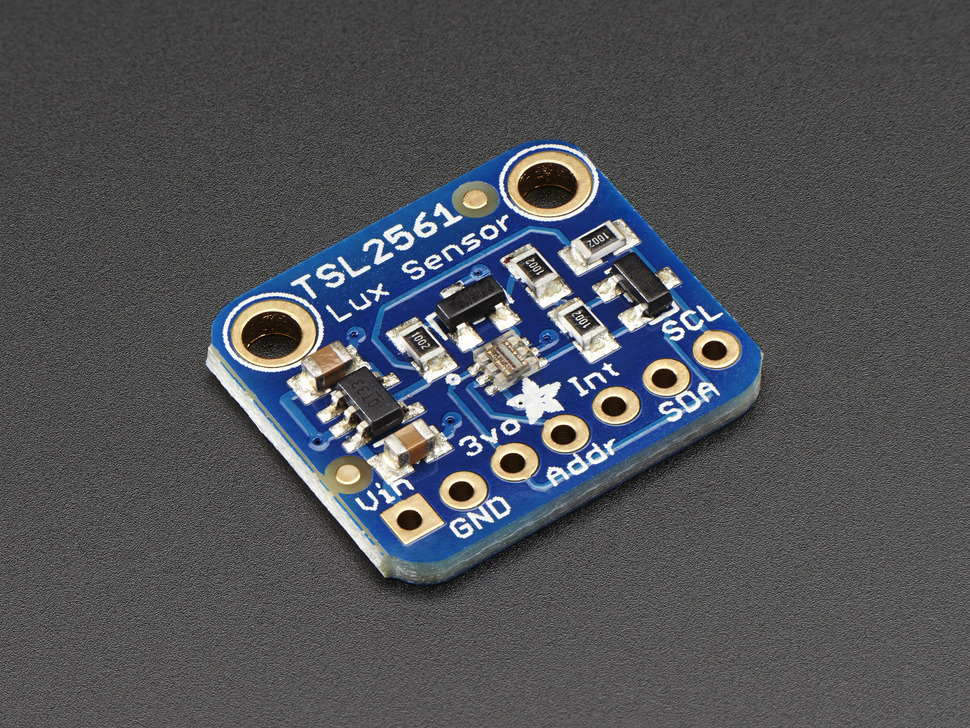
\includegraphics[width=0.5\textwidth]{graphics/TSL2561/TSL2561_Breakout.JPG}
\captionof{figure}{TSL2561 Breakout Board von Adafruit \cite{TSL2561Adafruit}}
\label{fig:TSL}
\end{figure}

\begin{table}[h]
  \centering
  \caption{Elektrische Spezifikationen des TSL2561 \cite{TSL2561}}
    \begin{tabular}{lllll}
    \toprule
    \textbf{Parameter} & \textbf{Min.} & \textbf{Typ.} & \textbf{Max.} & \textbf{Einheit} \\
    \midrule
    Versorgungsspannung & 2.7  & 3   & 3.6   & V \\
    Stromverbrauch (Aktiv) &       & 0.24   & 0.6   & mA \\
    Stromverbrauch inaktiv (Power down) &       & 3.2   & 15 & $\mu$A \\
    \bottomrule
    \end{tabular}%
  \label{tab:TSL2561}%
\end{table}%
\newpage
\subsubsection{BME280}
Im Verlauf der Bachelor-Thesis wurde über das Design des Gehäuses der Wetterstation diskutiert, dabei wurde ebenfalls die Notwendigkeit eines Zugangs zu frischer Umgebungsluft für den BME280 erwähnt. Würde der BME280 auf dem PCB angebracht werden, so würde dieser durch die Abwärme der Elektronik stärker beeinflusst und Fehlmessungen generieren. Aus diesem Grund soll der BME280 an der unteren Seite des Gehäuses, zugänglich zu frischer Aussenluft, montiert werden. Damit Fehlmessungen möglichst vermieden werden können, wird wie beim TSL2561 für den BME280 ein Breakout Board verwendet (Abbildung \ref{fig:BME_Breakout}) und über Pinheader mit dem PCB verbunden.\\

\begin{figure}[hbtp]
\centering
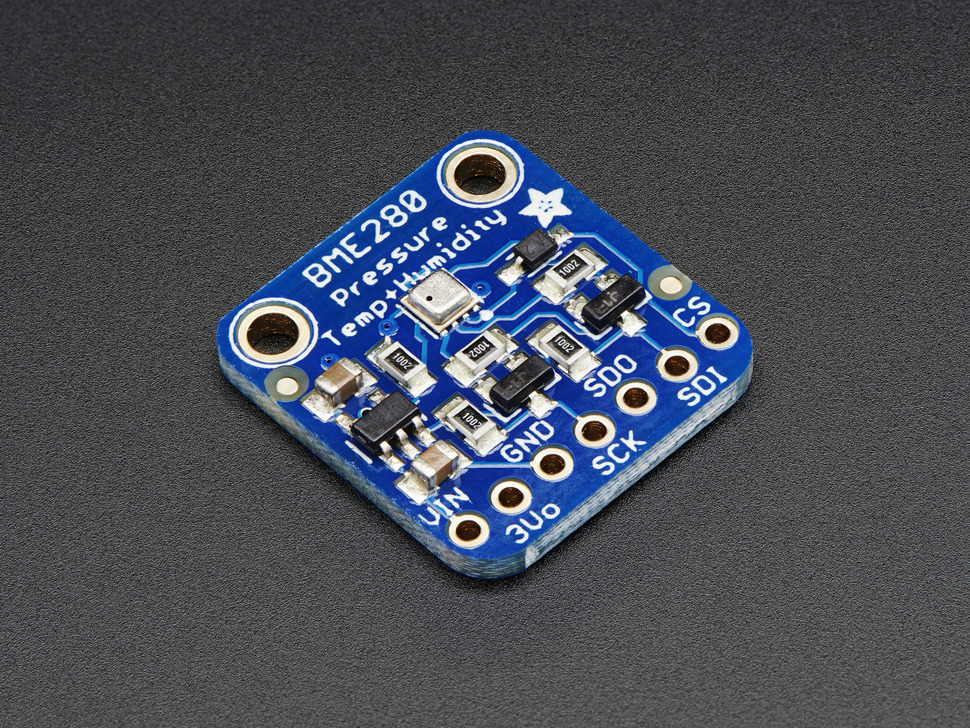
\includegraphics[width=0.5\textwidth]{graphics/BME280/BME280_Breakout.JPG}
\captionof{figure}{BME280 Breakout Board von Adafruit \cite{BME_Breakout}}
\label{fig:BME_Breakout}
\end{figure}

Die gesammelten Daten der Sensorik werden an die MCU geliefert. Die MCU kann jedoch nicht alle Daten speichern, weshalb ein grösserer, externer Speicher notwendig ist. Aus diesem Grund wird im nächsten Kapitel auf die Datenspeicherung eingegangen.
\subsection{Datenspeicherung}
\label{subsec:Datenspeicherung}
Während des Projekt 5 wurde die Datenspeicherung bereits mittels Breakout Board im Prototyp implementiert. Nachfolgend wird die Dokumentation aus dem Fachbericht des Projekt 5 übernommen und in einem weiteren Abschnitt Ergänzungen dazu aus der Bachelor-Thesis erläutert.

\subsubsection{Datenspeicherung - Projekt 5}
Die Datenspeicherung beinhaltet die gespeicherten Messwerte der Sensoren. Die Daten werden dann in einem *.txt-File nicht flüchtig gespeichert. Bei Beschädigung der Hardware können dann die zuletzt erfassten Daten immer noch mittels eines SD-Karten-Adapters von einem Computer ausgelesen werden. Als Kommunikationsprotokoll für das Schreiben und Auslesen der Karte wird SPI verwendet.

\subsubsection*{$\mu$SD-Karte}
\begin{minipage}{0.44\textwidth}
\centering
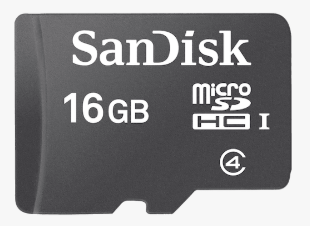
\includegraphics[width=0.4\textwidth]{graphics/Datenspeicherung/micro_sd_card_16GB.png}
\captionof{figure}{16 GB $\mu$SD-Karte \cite{musdkarte}}
\label{fig:muSDKarte}
\end{minipage}
\begin{minipage}{0.55\textwidth}
Bei der $\mu$SD-Karte muss auf die Kompatibilität mit dem Breakoutboard geachtet werden. Dafür sind folgende Kriterien zu beachten:\\
\begin{itemize}
\item Die $\mu$SD-Karte muss FAT16 oder FAT 32 formatiert sein.
\item Es sind nur die SD und SD High Capacity (SDHC) kompatibel.\\
\end{itemize}
\end{minipage}
Für die Umsetzung dieses Projektes wurde eine $\mu$SD-Karte der SD-Familie SDHC \Romannum{1} verwendet (siehe Abb. \ref{fig:muSDKarte}). SDHC sind Kapazitäten bis zu 32GB möglich und FAT32 formatiert. \cite{muSDspez}\\ 
Die Grösse eines Strings lässt sich nach der Gleichung \ref{equ:berechnung_stringgroesse} berechnen, wenn angenommen wird, dass jeder Buchstaben (char) 8 Bit hat und zum Schluss noch ein Terminator für das Stringende angehängt wird:
\begin{equation}
\centering
Anzahl\ Zeichen * 1\ Byte + 1 = String\ Grösse\ in\ Byte
\label{equ:berechnung_stringgroesse}
\end{equation}
Bei einer Speicherung der Daten nach der Struktur in Abb. \ref{fig:datenausgabe} würden somit leicht aufgerundet ca. 216 Byte pro Speichersatz benötigt werden.\\
\todo{Kontrolle ref fig:datenausgabe}
Da momentan eine 16GB grosse $\mu$SD-Karte verwendet wird, ergeben sich daraus
\begin{equation}
\dfrac{16E9}{216}=74.1E6 \approx \underline{\underline{74E6}}
\end{equation}
Speichersätze. Würden in einem zehn Minuten Zeitintervall ein Speichersatz abgespeichert werden, dann könnten 1411 Jahre 40 Wochen 4 Tage 21 Stunden 20 Minuten lang Werte von der Wetterstation abgespeichert werden. Diese Anzahl könnte noch verdoppelt werden, da wie oben bereits erwähnt $\mu$SD-Karten bis zu 32GB kompatibel sind.\\
\newpage
\subsubsection{Ergänzungen aus der Bachelor-Thesis}
Im Gegensatz zum Prototyping wird für die endgültige Wetterstation kein Breakout Board mehr verwendet. Die $\mu$SD-Karte wird in ein $\mu$SD-Karten-Adapter (Speicherkartenverbinder) gesteckt, welcher über ein Buffer (74HC4050) mit der MCU verbunden ist (siehe Abbildung \ref{fig:Uebersicht_PCB_MCU_RTC_SD_Sense}). Der 74HC4050 kann als Levelshifter verwendet werden und als Treiber für kapazitive Ladungen. In unserem Fall werden MCU und Speicherkartenverbinder mit 3.3V betrieben, weshalb kein Levelshifter notwendig ist. Der 74HC4050 wird demnach bei der Wetterstation als Treiber für kapazitive Ladungen verwendet.\\

Die Daten werden mit der Sensorik ermittelt, über die MCU verarbeitet und in der $\mu$SD-Karte gespeichert. Nun sollen die Daten jedoch per SMS (GSM) abrufbar sein und die Wetterstation ebenfalls über ein GPS-Modul verfügen. Aus diesem Grund wird im nächsten Kapitel auf die Kommunikationsmodule (GSM, GPS) eingegangen.
 
\subsection{Kommunikationsmodule}
\label{subsec:Kommunikationsmodule}
Gemäss Auftraggeber sollen Daten der Wetterstation per SMS abrufbar und der Standort der Wetterstation ermittelbar sein. Um SMS empfangen und auch senden zu können, wird ein GSM-Modul benötigt. Weiter wird ein GPS-Modul benötigt, um eine Standortermittlung durchführen zu können. Der SIM808 ist ein Kombinationsmodul aus GSM und GPS, was nicht nur Platz auf dem PCB, sondern auch Energietechnisch und Preislich Vorteile bietet, da nur ein Modul betrieben werden muss. Aus diesen Gründen wurde der SIM808 implementiert.

\subsubsection{SIM808}
{\begin{minipage}[b][6cm][t]{0.52\textwidth}
Der SIM808 (Abbildung \ref{fig:SIM808}) verfügt über GSM/GPRS (Global System for Mobile Communications / General Packet Radio Service), GPS (Global Positioning System) und BT (Bluetooth). Für die Wetterstation wird das GSM und das GPS verwendet. Tabelle \ref{tab:SIM808} zeigt die elektrischen Spezifikationen des SIM808. \cite{SIM808}\\
\end{minipage}}
{\begin{minipage}[b][6cm][t]{0.47\textwidth}
\centering
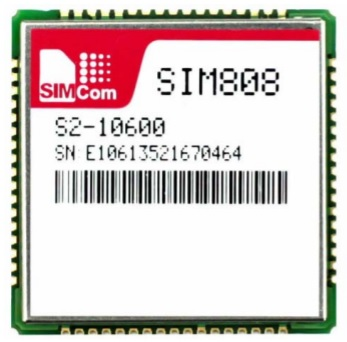
\includegraphics[width=0.7\textwidth]{graphics/SIM808/SIM808.JPG}
\captionof{figure}{SIM808 von Vorne 
\cite{SIM808}}
\label{fig:SIM808}
\end{minipage}}


\begin{table}[h]
\centering
  \caption{Elektrische Spezifikationen des SIM808 \cite{SIM808}}
\begin{tabular}{lllll}
\toprule 
\textbf{Parameter} & \textbf{Min} & \textbf{Typ} & \textbf{Max} & \textbf{Einheit} \\ 
\midrule 
Power Supply & 3.4 &  & 4.4 & V \\ 
Power saving &  & 1 &  & mA \\ 
Transmitting power (GSM) &  & 2 &  & W \\ 
SIM interface support &  & 1.8/3 &  & V \\ 
Power consumption (Idle GSM) &  & 22.1 &  & mA \\
Power consumption (Data GSM) &  & 445.82 &  & mA \\
Power consumption (TX Burst GSM) &  &  & 2 & A \\
Power consumption (GPS Acquisition) &  & 42 &  & mA \\ 
Power consumption (GPS Continuous tracking) &  & 24 &  & mA \\ 
\bottomrule
\end{tabular} 
\label{tab:SIM808} 
\end{table}

Damit das GSM über den SIM808 genutzt werden kann, wird eine SIM-Karte benötigt. Dafür wurde eine Prepaid M-Budget SIM-Karte von Andres Minder erworben, welche jedoch Vertragsbedingt persönlich ist und nicht Teil der Wetterstation bleibt. Diese SIM-Karte wird lediglich zu Testzwecken genutzt und muss später durch eine SIM-Karte des Endbenutzers ersetzt werden. Die SIM-Karte wird mit einem SIM-Karten-Adapter (Speicherkartensteckverbinder) auf dem PCB integriert und mit dem SIM808 verbunden.
\newpage
Wie in der Übersicht zu sehen ist (Abbildung \ref{fig:Uebersicht_PCB_USB_SIM}), benötigt die SIM808 zwei verschiedene Antennen. Eine Antenne für das GSM, die andere für das GPS. Diese Antennen sind standardisiert und können direkt online erworben werden. Die Energieversorgung des SIM808 benötigt eine Schaltung aus Kondensatoren und einer Diode, welche die Spannung des Akkus von möglichen Störungen befreit und den SIM808 vor Überspannung schützt. Der verwendete 74VHC125 wird als Pegelwandler verwendet, da die SIM808 mit einer höheren Spannung betrieben wird als die MCU. Ausserdem schützen Dioden den RST- und RX-Pin des SIM808 vor ungewollten Spannungsspitzen und deren Folgen (z.B. das Auslösen eines Reset). Die SIM-Karte wird in einem entsprechenden Adapter über ein Schutzdioden-Array mit dem SIM808 verbunden. Das Schutzdioden-Array schützt ebenfalls die SIM-Karte vor Überspannungen, indem diese über die Ground-Plane abgeleitet werden. Zwei Status-LED zeigen den Betrieb der SIM808 und dessen Konnektivität.\\[0.5cm]
Die verschiedenen Systeme wurden erläutert, wobei die Energieversorgung bereits öfter angesprochen und nie thematisiert wurde. Im nächsten Kapitel soll dies nachgeholt und die Energieversorgung detailiert erläutert werden.


\subsection{Energieversorgung}
\label{subsec:Energieversorgung}
Die verschiedenen Bauteile auf dem PCB müssen mit Energie versorgt werden. Gemäss Auftragsbeschreibung soll die Wetterstation desweiteren über Photovoltaik gespiesen werden. Da die Sonne nur tagsüber scheint und um eine konstante Versorgung gewährleisten zu können, wird ein Akku benötigt. Um die Speisung via Akku und gleichzeitig ein Speisen des Akkus über die Photovoltaikanlage zu gewährleisten, muss der Ladestrom geregelt werden, was mit einem Power-Management-IC, dem MCP73871, erfolgt. Der MCP73871 führt die Speisung des Akkus weiter auf einen Linearregler (LM1117), welcher das 3.3V-Netz generiert. Damit der LM1117 eine saubere Ausgangsspannung (3.3V mit möglichst kleinem Rippel) generieren kann, muss dieser einen erhöhten Spannungspegel am Eingang haben, weshalb eine ChargePump (Ladungspumpe) benötigt wird. Das Konzept der Energieversorgung wird in Kapitel \ref{sec:Konzept} vorgestellt, weshalb nun die Berechnung der Akkukapazität, der Einfluss der Photovoltaik, sowie die Kombination von ChargePump und Linearregler näher erläutert werden.
%\subsubsection{Energiekonzept}
%\label{subsubsec:Energiekonzept}
%In diesem Kapitel wird das Energiekonzept erläutert. Dies soll eine Übersicht über die Energieversorgung geben.\\
%\begin{figure}[hbtp]
%\centering
%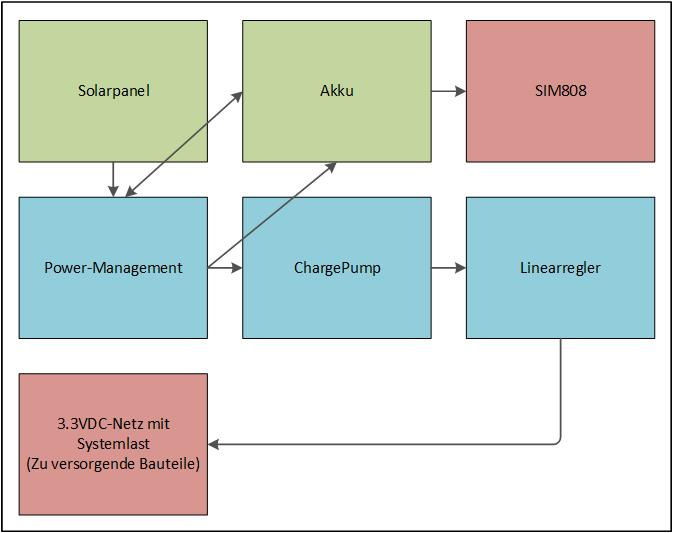
\includegraphics[width=0.8\textwidth]{graphics/Energieversorgung/Konzept.JPG}
%\captionof{figure}{Konzept der Energieversorgung}
%\label{fig:Energiekonzept}
%\end{figure}\\
%\newpage
%Abbildung \ref{fig:Energiekonzept} zeigt das Konzept der Energieversorgung. Darin sind Grün markiert die Energielieferanten, Blau die Schaltung um das 3.3V-Netz zu generieren und Rot die Verbraucher. Das Solarpanel speist über das Power-Management (MCP73871) den Akku. Der Akku ist die Quelle für die gesamte Wetterstation und speist diese ebenso über den MCP73871. Die Spannung des Akkus wird über den MCP73871 auf die ChargePump gegeben und dort erhöht, so dass der nachfolgende Linearregler (LM1117) mit dieser erhöhten Spannung einen möglichst konstanten (rippelfreien) 3.3V-Ausgang generiert. Mit diesem Ausgang des LM1117 wird das 3.3V-Netz generiert, woraus die benutzten Bauteile (die Systemlast) ihre benötigte Spannung erhalten. Einzige Ausnahme bildet hier der SIM808, da dieser eine höhere Spannung benötigt. Da der SIM808 eine erhöhte Betriebsspannung hat und Stromspitzen für das Senden und Empfangen von SMS aufweist, wird dieser direkt über den Akku betrieben. Falls die Wetterstation nicht benötigt werden sollte, können die Verbraucher über ein Schalter abgeschaltet werden. Es ist zu beachten, dass das Benutzen des Schalters die Energieversorgung sofort komplett trennt und auf dem PCB diverse Kondensatoren vorhanden sind, welche sich noch entladen. Ausserdem wird der MCP73871 nicht ausgeschaltet, weshalb ein weiteres laden des Akkus über die Photovoltaik möglich ist.
\subsubsection{Berechnung der Akkukapazität}
Um die Kapazität des Akkus zu berechnen, muss eine Schätzung des Energieverbrauchs gemacht werden. In Tabelle \ref{tab:Energieverbrauch} werden deshalb die verwendeten Bauteile mit ihrem Stromverbrauch aufgelistet.
\begin{table}[h]
	\centering
	\caption{Übersicht über die verwendeten Bauteile mit ihrem Stromverbrauch.}
	\small
  \begin{tabular}{lllllll}
  \toprule 
  \textbf{Bauteilname} & \textbf{Modus} & \textbf{Min} & \textbf{Typ} & \textbf{Max} & \textbf{Einheit}\\ 
  \midrule 
  MCP73871 \cite{MCP73871}& Charge Complete &  & 120 & 200 & $\mu$A  \\ 
  \hline 
  LM1117 \cite{LM1117} &  & & 5 & 10 & mA   \\ 
  \hline 
  SIM808 \cite{SIM808}& PWR Down &  & 38 & 50 & $\mu$A   \\ 
   & Idle  &  & 22.1 &  & mA  \\ 
   & Data GSM &  & 445.82 &  & mA   \\ 
   & GPS acquisition &  & 42 &  & mA   \\ 
   & GPS continuous tracking &  & 24 &  & mA   \\ 
   & TX Burst (peak)  &  & 2 &  & A  \\ 
  \hline 
  Anemometer &  &  &  &  &   \\ 
  \hline 
  Ombrometer &  &  &  &  &   \\ 
  \hline 
  Windrichtungsgeber \cite{ADSkeineAngabe}&  & 0.028 &  & 4.8 & mA \\ 
  \hline 
  74VHC125 \cite{74HC125}&  & 20 &  & 40 & $\mu$A  \\ 
  \hline 
  ATMega2560 \cite{arduinoMega}& active &  & 7 &  & mA  \\ 
  \hline
  PN2222A & active &  & 600 &  & mA  \\
  \hline 
  FT231XS \cite{FTDI}& normal & 8 & 8 & 8.4 & mA \\ 
   & USB suspend &  & 125 &  & $\mu$A \\ 
  \hline 
  74HC4050 \cite{74HC4050}&  &  &  & 40 & $\mu$A \\ 
  \hline 
  BME280 \cite{Bosch2019}& standby &  & 0.2 & 0.5 & $\mu$A  \\ 
   & humidity measuring &  & 340 &  & $\mu$A \\ 
   & pressure measuring &  & 714 &  & $\mu$A  \\ 
   & temperature measuring &  & 350 &  & $\mu$A \\ 
  \hline 
  TSL2561 \cite{TSL2561}& active &  & 0.24 & 0.6 & mA \\ 
   & power down &  & 3.2 & 15 & $\mu$A  \\ 
  \hline 
  DS3231 \cite{DS3231DS}& active & &  & 200 & $\mu$A \\ 
   & standby &  & & 110 & $\mu$A  \\ 
  \bottomrule 
  \end{tabular} 
	\label{tab:Energieverbrauch} 
\end{table}
\newpage
Tabelle \ref{tab:Energieverbrauch} zeigt den Stromverbrauch der verwendeten Bauteile gemäss ihren Datenblättern. Das Anemometer und das Ombrometer besitzen keine Werte, da nur beim Schliessen eines der integrierten Reedkontakte ein Strom fliesst, weshalb diese Ströme vernachlässigt werden. Die Ströme des Windrichtungsgebers wurden berechnet anhand der 3.3V Versorgungsspannung und den Widerstandswerten gemäss Datenblatt. Vom MCP73871 wurde lediglich der Strom bei geladenem Akku genommen, da das Laden des Akkus mit dem Ladestrom der Photovoltaik erfolgt und somit nicht direkt ein Verbrauch ist. Der SIM808 besitzt mit seinen 2A Spitzenstrom bei einem TX Burst (senden einer SMS) den höchsten Konsum, jedoch ist dieser Burst lediglich 577$\mu$s lang und wird somit auch nicht berücksichtig, zumal nicht gesagt werden kann wie oft dieser Burst tatsächlich vorkommt. Der SIM808 wird im Normalbetrieb das GPS im continuous tracking und das GSM im Idle Modus haben, weshalb hier insgesamt ein Strom von Typ 46,1 mA verbraucht wird. Der ATMega2560 wird im Normalbetrieb stets im active Modus sein, weshalb nur dieser Wert aus dem Datenblatt ausgelesen wurde. Die serielle Schnittstelle wird im Normalbetrieb nicht benutzt (kein Notebook angehängt), weshalb beim FT231XS der USB suspend Modus zur Berechnung benutzt und der PN2222A vernachlässigt wird. Der BME280 sollte stets Messungen durchführen, weshalb hier mit dem höchsten Wert (pressure measuring Modus) gerechnet wird. Ähnlich verhält es sich beim TSL2561 und beim DS3231, hier werden die active Modi in die Rechnung mit einbezogen.\\[0.5cm]
Um den SIM808 mit einer optimalen Spannung versorgen zu können, wird ein Akku mit einer Spannung von 4V benötigt. Der Gesamtstrombedarf im Normalbetrieb beläuft sich gemäss Tabelle \ref{tab:Energieverbrauch} und verwendeten Maximalwerten auf rund 70mA. Multipliziert man die Spannung mit dem Gesamtstrombedarf, so ergibt dies eine Leistung von 0.28 Watt. Um daraus die benötigte Akkukapazität zu ermitteln, muss festgelegt werden, wie lange dieser die Wetterstation mindestens speisen können soll. Gemäss Pflichtenheft soll der Akku die Wetterstation für mindestens 100 Stunden aufrecht erhalten können. Die berechnete Leistung wird mit den Anzahl Stunden multipliziert, was 28 Wh ergibt. Bei einer Akkuspannung von 4V ergibt das (durch dividieren der 28 Wh mit den 4V) eine Mindest-Akkukapazität von 7Ah oder auch 7000mAh.
\subsubsection{Einfluss der Photovoltaik}
Die Photovoltaik (das Solarpanel) erzeugt Strom durch Sonnenenergie. Der erzeugte Strom wird dazu verwendet den Akku zu laden, während dieser die Wetterstation speist. Im vorhergehenden Kapitel wurde die benötigte Leistung der Wetterstation von 0.28 Watt berechnet und die daraus Resultierende Mindest-Akkukapazität von 7000mAh. Gemäss Pflichtenheft soll das Solarpanel den Akku innert einem Tag laden können.\\

\begin{figure}[h]
\centering
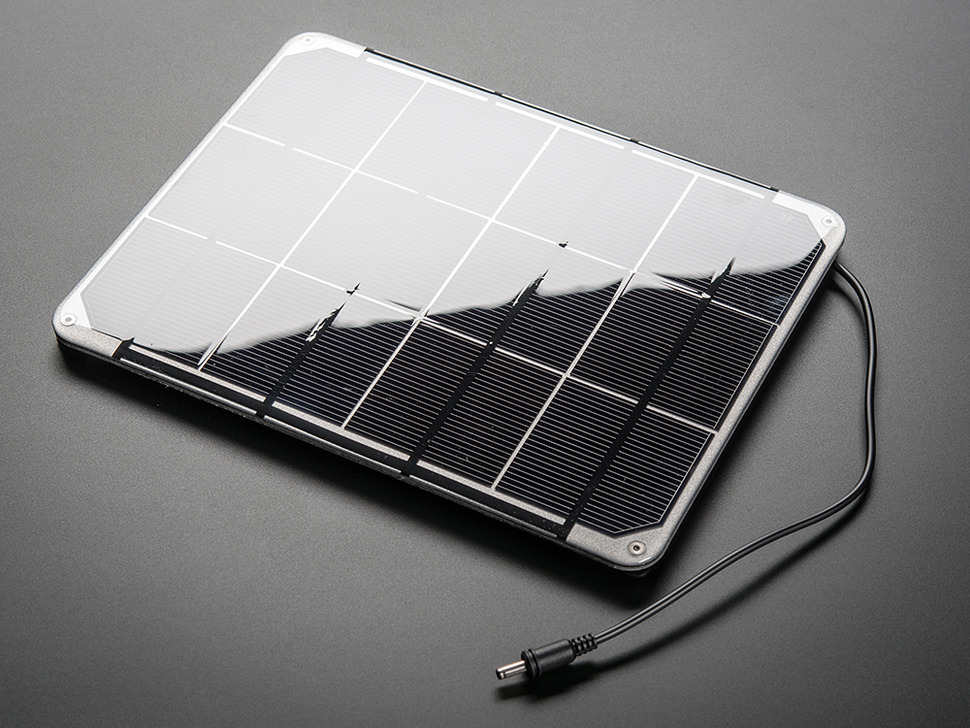
\includegraphics[width=0.4\textwidth]{graphics/Energieversorgung/Solarpanel.JPG}
\captionof{figure}{6V 6W Solarpanel von Adafruit \cite{Solarpanel}}
\label{fig:Solarpanel}
\end{figure}
\newpage
Da das Solarpanel nur bei Sonneneinstrahlung Strom erzeugen kann und die Sonnenstunden von Land zu Land abweichen, werden bei dieser Rechnung 6 Sonnenstunden pro Tag angenommen. Um 7000mAh innert 6h laden zu können, müssen konstant 1166.66mA bzw. rund 1.2A Strom erzeugt werden. Hier beschränkt jedoch der MCP73871, da dieser bei dementsprechender Beschaltung ein Fast Charge Current von Typ 1A und Max 1.1A zulässt. Rechnet man zurück so wird das Solarpanel typischerweise 7h benötigen um bei einem erzeugten Ladestrom von 1A den Akku voll zu laden. Während den Sommermonaten sollte dies in den meisten Gegenden kein Problem darstellen, doch könnte dies über die Wintermonate nicht reichen. Um dies zu verifizieren rechnen wir den Verbrauch der Schaltung pro Tag aus und schauen, wie viele Sonnenstunden das Solarpanel bräuchte um bei 1A Ladestrom den Verbrauch auszugleichen. Bei 0.28W Verbrauch und 24h pro Tag ergibt das 6.72Wh. Da der Akku 4V liefert folgen daraus 1.68Ah Verbrauch für den Akku. Geht man wieder von einem Ladestrom von 1A aus, so werden 1.68 Sonnenstunden benötigt bei denen das Solarpanel 1A Ladestrom erzeugt um den Verbrauch zu decken. Aus diesem Grund kann gesagt werden, dass jedes Solarpanel wegen des MCP73871 nicht ausreichen wird, um die Mindest-Akkukapazität von 7000mAh innert 6 Sonnenstunden laden zu können. Wird jedoch ein Solarpanel verwendet das 1A Ladestrom erzeugen kann, so werden lediglich 1.68 Sonnenstunden benötigt um den Verbrauch zu decken. Für die Wetterstation wurde ein 6V 6W Solarpanel von Adafruit implementiert (Abbildung \ref{fig:Solarpanel}, was somit 1A Ladestrom erzeugen kann und ausreicht um den Verbrauch der Wetterstation innert 1.68 Sonnenstunden zu decken \cite{Solarpanel}.\\

\subsubsection{ChargePump und Linearregler}
Die Wetterstation besteht aus einigen Bauteilen, welche eine 3.3V-Versorgungsspannung benötigen. Da der Akku eine höhere Spannung liefert, muss ein Linearregler die Spannung auf 3.3V regeln. Dafür wird der LM1117 verwendet, welcher eine Eingangsspannung von bis zu Max 15V aushält. Damit der LM1117 die Eingangsspannung sauber (möglichst ohne Rauschen) auf die 3.3V regeln kann, sollte die Eingangsspannung mindestens 5V betragen. Um von den 4V Batteriespannung auf mindestens 5V zu gelangen, wird eine ChargePump verwendet. Eine ChargePump ist eine Schaltung, welche aus einem Schalter, 2 Kondensatoren und 2 Dioden besteht, wie in Abbildung \ref{fig:ChargePump} schematisch dargestellt. 

\begin{figure}[h]
\centering
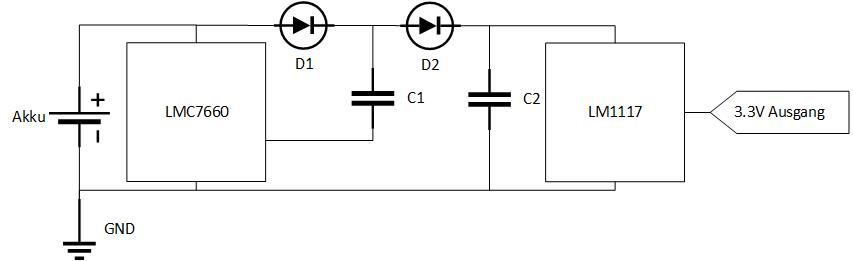
\includegraphics[width=1\textwidth]{graphics/Energieversorgung/ChargePump.JPG}
\captionof{figure}{Schematische Darstellung der ChargePump.}
\label{fig:ChargePump}
\end{figure}
\newpage
Abbildung \ref{fig:ChargePump} zeigt die Schematische Darstellung der verwendeten ChargePump. Als Schalter wird der LMC7660 verwendet, welcher zwischen 2 Stromkreisen wechselt. Das wechseln der Stromkreise bewirkt das aufladen des jeweiligen Kondensators. Im ersten Schalterzustand bilden D1, C1 und der Akku einen Stromkreis, wobei sich C1 auf die Akkuspannung lädt (abzüglich der Diodenspannung von D1). Im zweiten Zustand ist der Akku in Serie zu C1, welcher nun als Spannungsquelle fungiert, und der Kondensator wird auf die doppelte Akkuspannung (abzüglich der Diodenspannungen) geladen. In beiden Zuständen sorgen die Dioden dafür, dass sich der Kondensator kontrolliert auf die gewünschte Seite hin entlädt. Durch diese ChargePump soll im Idealfall eine Spannung von etwa 6.6V (Doppelte Akkuspannung von 8V abzüglich der zwei Diodenspannungen von je ca. 0.7V) generiert werden können. Durch diese erhöhte Spannung ist es dem LM1117 möglich die Spannung auf 3.3V zu regeln, wobei durch Toleranzen ein nur relativ kleiner Rippel entsteht. Die Spannung am Ausgang des Linearreglers ist Ausgangspunkt für die Speisespannungen der Bauteile, welche eine 3.3V-Speisespannung benötigen.\\[0.5cm]
Nun wurde die Energieversorgung ebenfalls detailiert erläutert. Auf die verschiedenen Bauteilgruppen wurden nun in den verschiedenen Kapiteln jeweils näher eingegangen. Im nächsten Kapitel wird deshalb die Realisierung der Wetterstation auf einem PCB (Printed Circuit Board) thematisiert.

\subsection{PCB}
\label{subsec:PCB}
Ein PCB (Printed Circuit Board, dt. Leiterplatte) beherbergt die verwendeten Bauteile und verbindet diese elektronisch miteinander. Die verwendeten Bauteile werden auf das PCB gelötet, wobei es SMD (Surface Mount Device) und THT (Trough Hole Technology) zu unterscheiden gilt. Wie der Name schon sagt, werden THT-Bauteile durch das PCB gesteckt und SMD-Bauteile lediglich auf die Oberfläche gelegt, wobei beide vorgesehene Lötstellen haben auf diese sie gelötet werden um elektrischen Kontakt über Leiterbahnen zu erstellen.
Das PCB und das dazugehörige Schema werden in einem EDA-Programm (Electronic Design Automation) erstellt. Für die Wetterstation wurde das Programm EAGLE (Einfach Anzuwendender Grafischer Layout-Editor) der Firma Autodesk verwendet, wegen der im Namen schon angedeuteten einfachen Anwendung. Für die Wetterstation wurde ein 4-Lagen-PCB ausgewählt, da dies im Vergleich zu einem 2-Lagen-PCB zu einem einfacheren Entwurf verhilft, hauptsächlich in Bezug zu Stromrückflüssen und EMV. Das Schema und das dazugehörige PCB-Layout sind im Anhang zu finden (Schema in Kapitel \ref{Anhang:Schema}, PCB-Layout in Kapitel \ref{Anhang:PCB}). Dem Anhang ist zu entnehmen, dass der erste und der vierte Layer für Signale bestimmt sind, der dritte Layer für die Versorgung (+3.3V) und der zweite Layer für das Ground (0V). In den nachfolgenden Abschnitten wird auf das Bestücken der Leiterplatte eingegangen und auf Mängel der ersten Version hingewiesen, sowie die Art und Weise wie diese Mängel behoben wurden.
\subsubsection{Das Bestücken der Leiterplatte}
{\begin{minipage}[b][6cm][t]{0.4\textwidth}
THT Bauteile werden durch das PCB durchgesteckt und von unten her angelötet. Nach dem anlöten werden die Beine, welche standardmässig relativ lang sind, möglichst nahe am PCB mit einem kleinen Seitenschneider gekürzt. In Abbildung \ref{fig:THT_Loeten} das Löten eines THT-Bauteils illustriert.
\end{minipage}}
{\begin{minipage}[b][6cm][t]{0.59\textwidth}
\centering
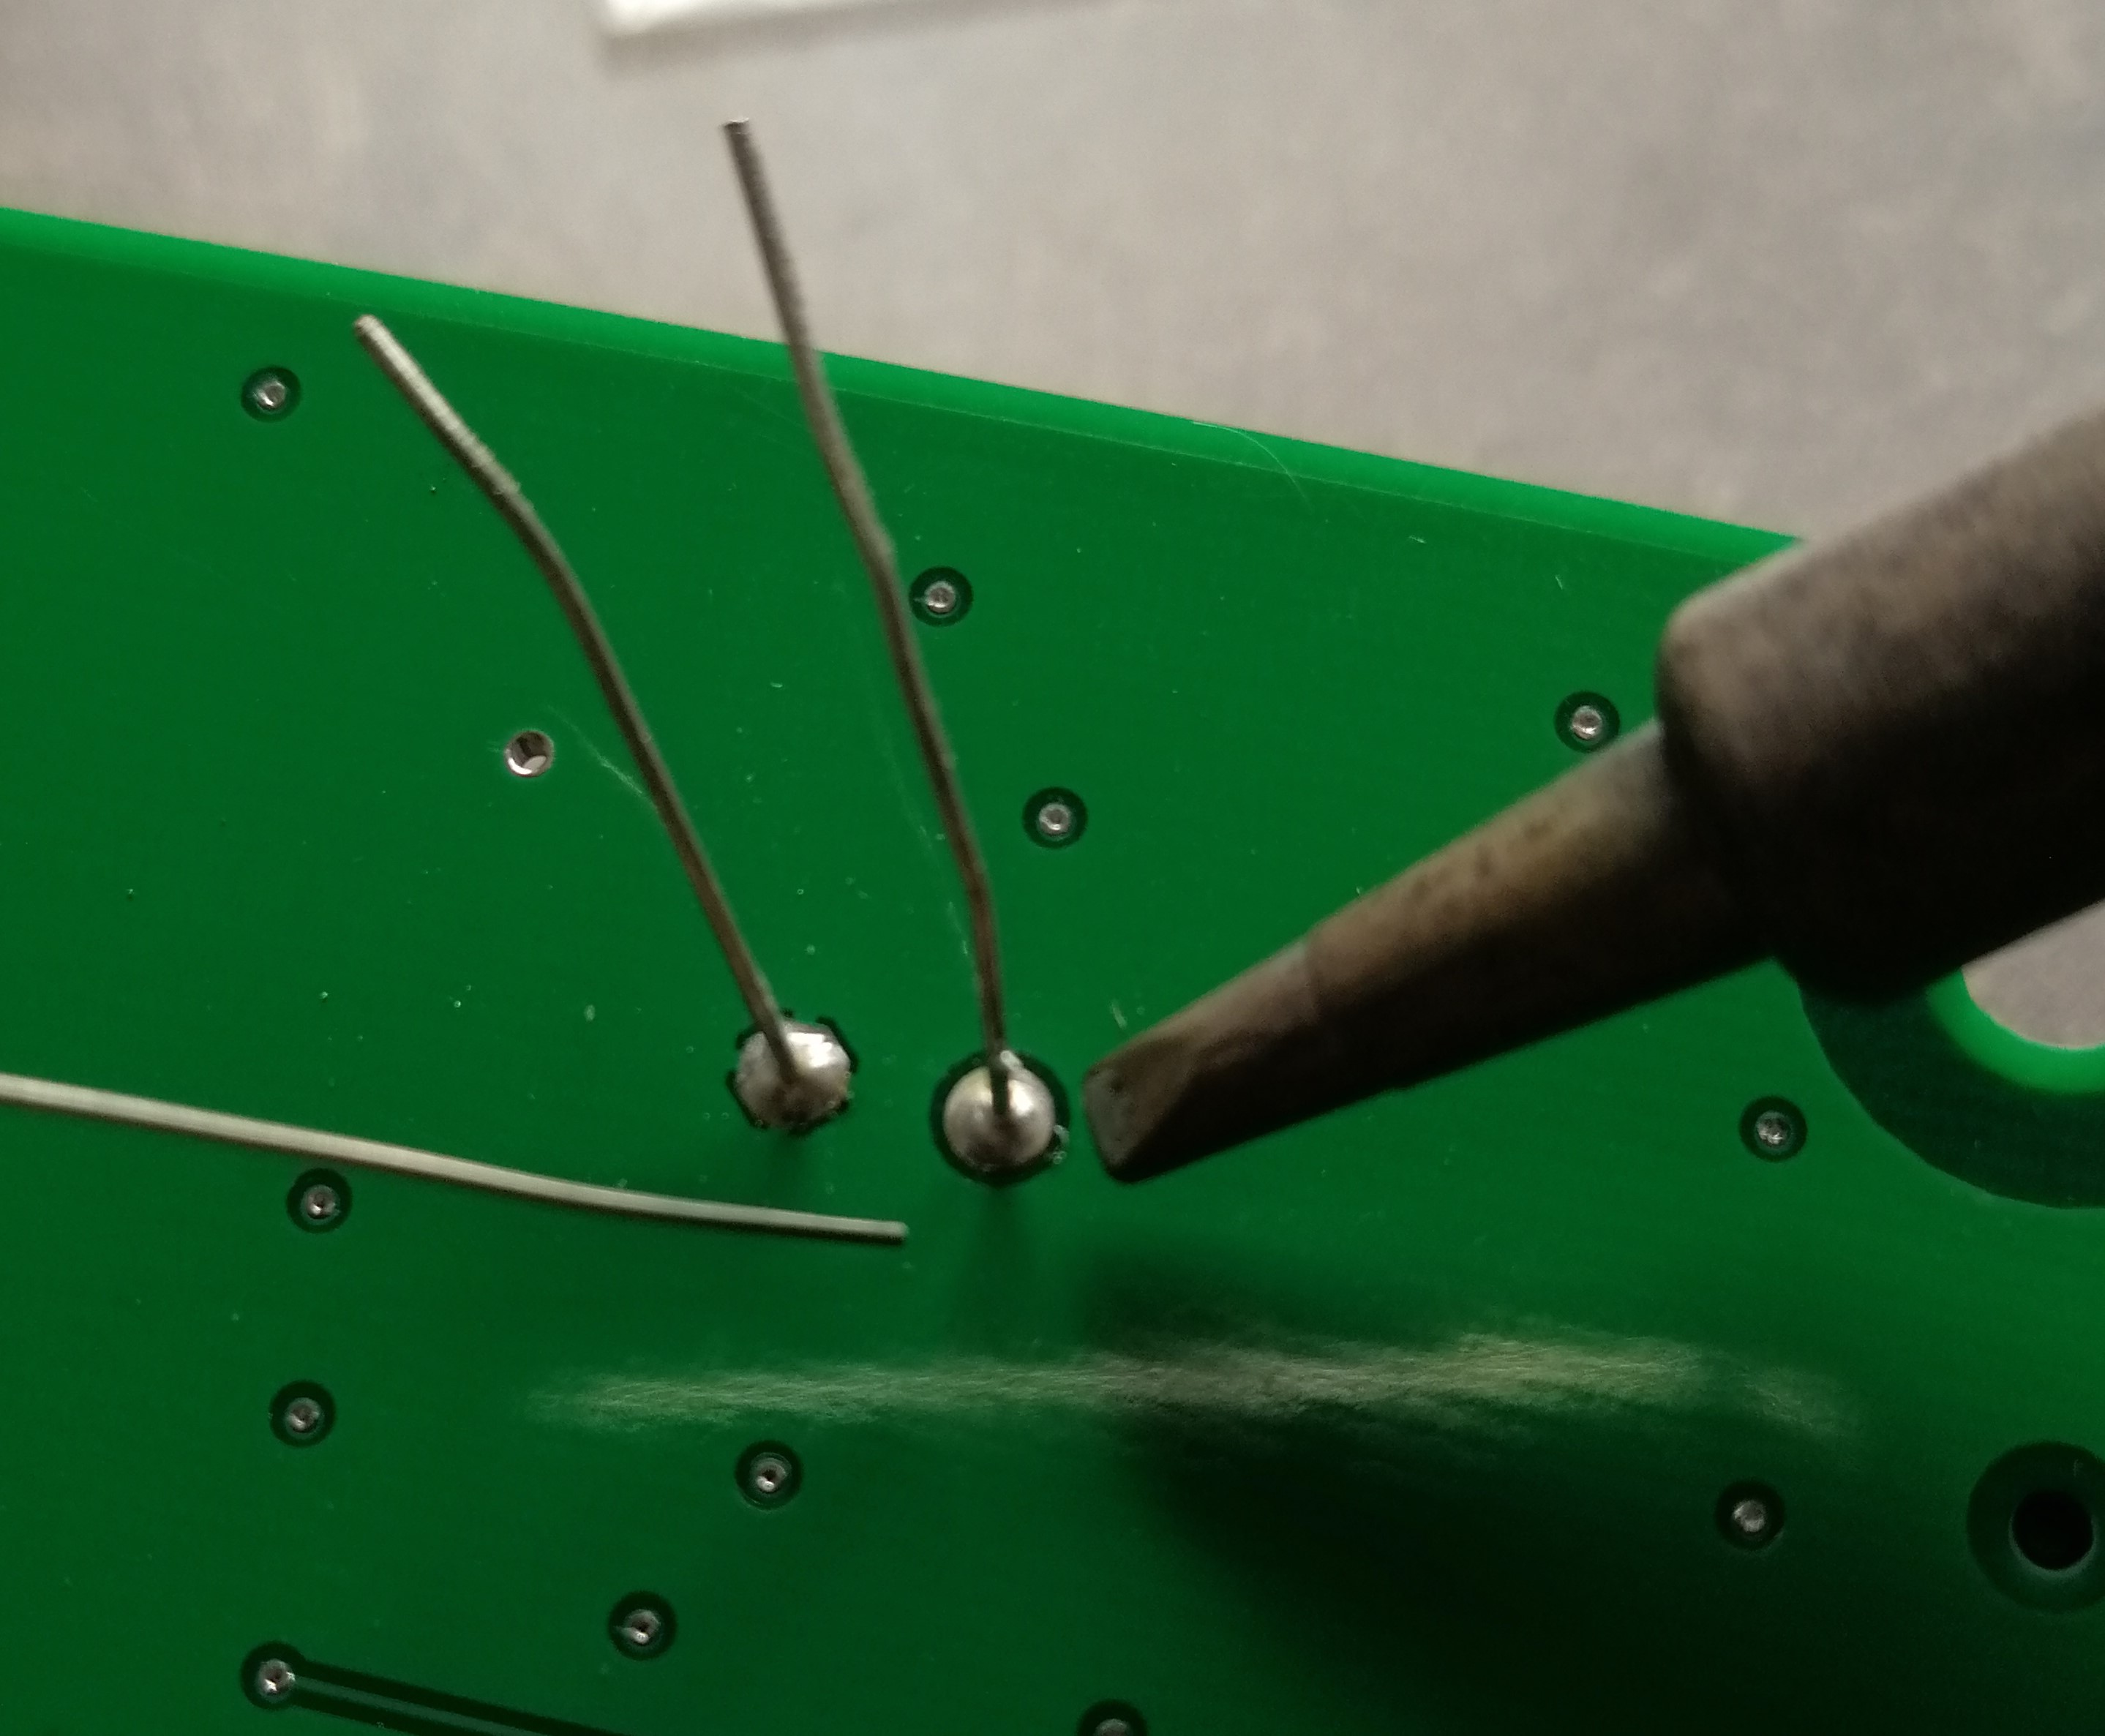
\includegraphics[width=0.7\linewidth]{graphics/HW_Val/THT_Loeten.jpg}
\captionof{figure}{Das Löten eines THT-Bauteils.}
\label{fig:THT_Loeten}
\end{minipage}}

{\begin{minipage}[b][8cm][t]{0.5\textwidth}
SMD Bauteile werden auf die Oberfläche des PCBs gelegt und dort angelötet. Dabei wird zuerst auf dem ersten Lötauge etwas Lötzinn aufgetragen. Mit einer Pinzette wird nun das SMD Bauteil korrekt platziert, während mit dem Lötstab der vorher aufgetragene Lötzinn flüssig gehalten wird. Ist das Bauteil korrekt platziert, wird es mit der Pinzette angedrückt, so dass es sich nicht verschiebt wenn der Lötstab entfernt wird und dieser dann entfernt, so dass der Lötzinn sich erhärtet und das Bauteil festhält. Nun kann von der anderen Seite her mit dem Lötstab das Lötauge erhitzt und mit Lötzinn das Bauteil angelötet werden. Dieser Vorgang wird in Abbildung \ref{fig:SMD_Loeten} illustriert.
\end{minipage}}
{\begin{minipage}[b][8cm][t]{0.49\textwidth}
\centering
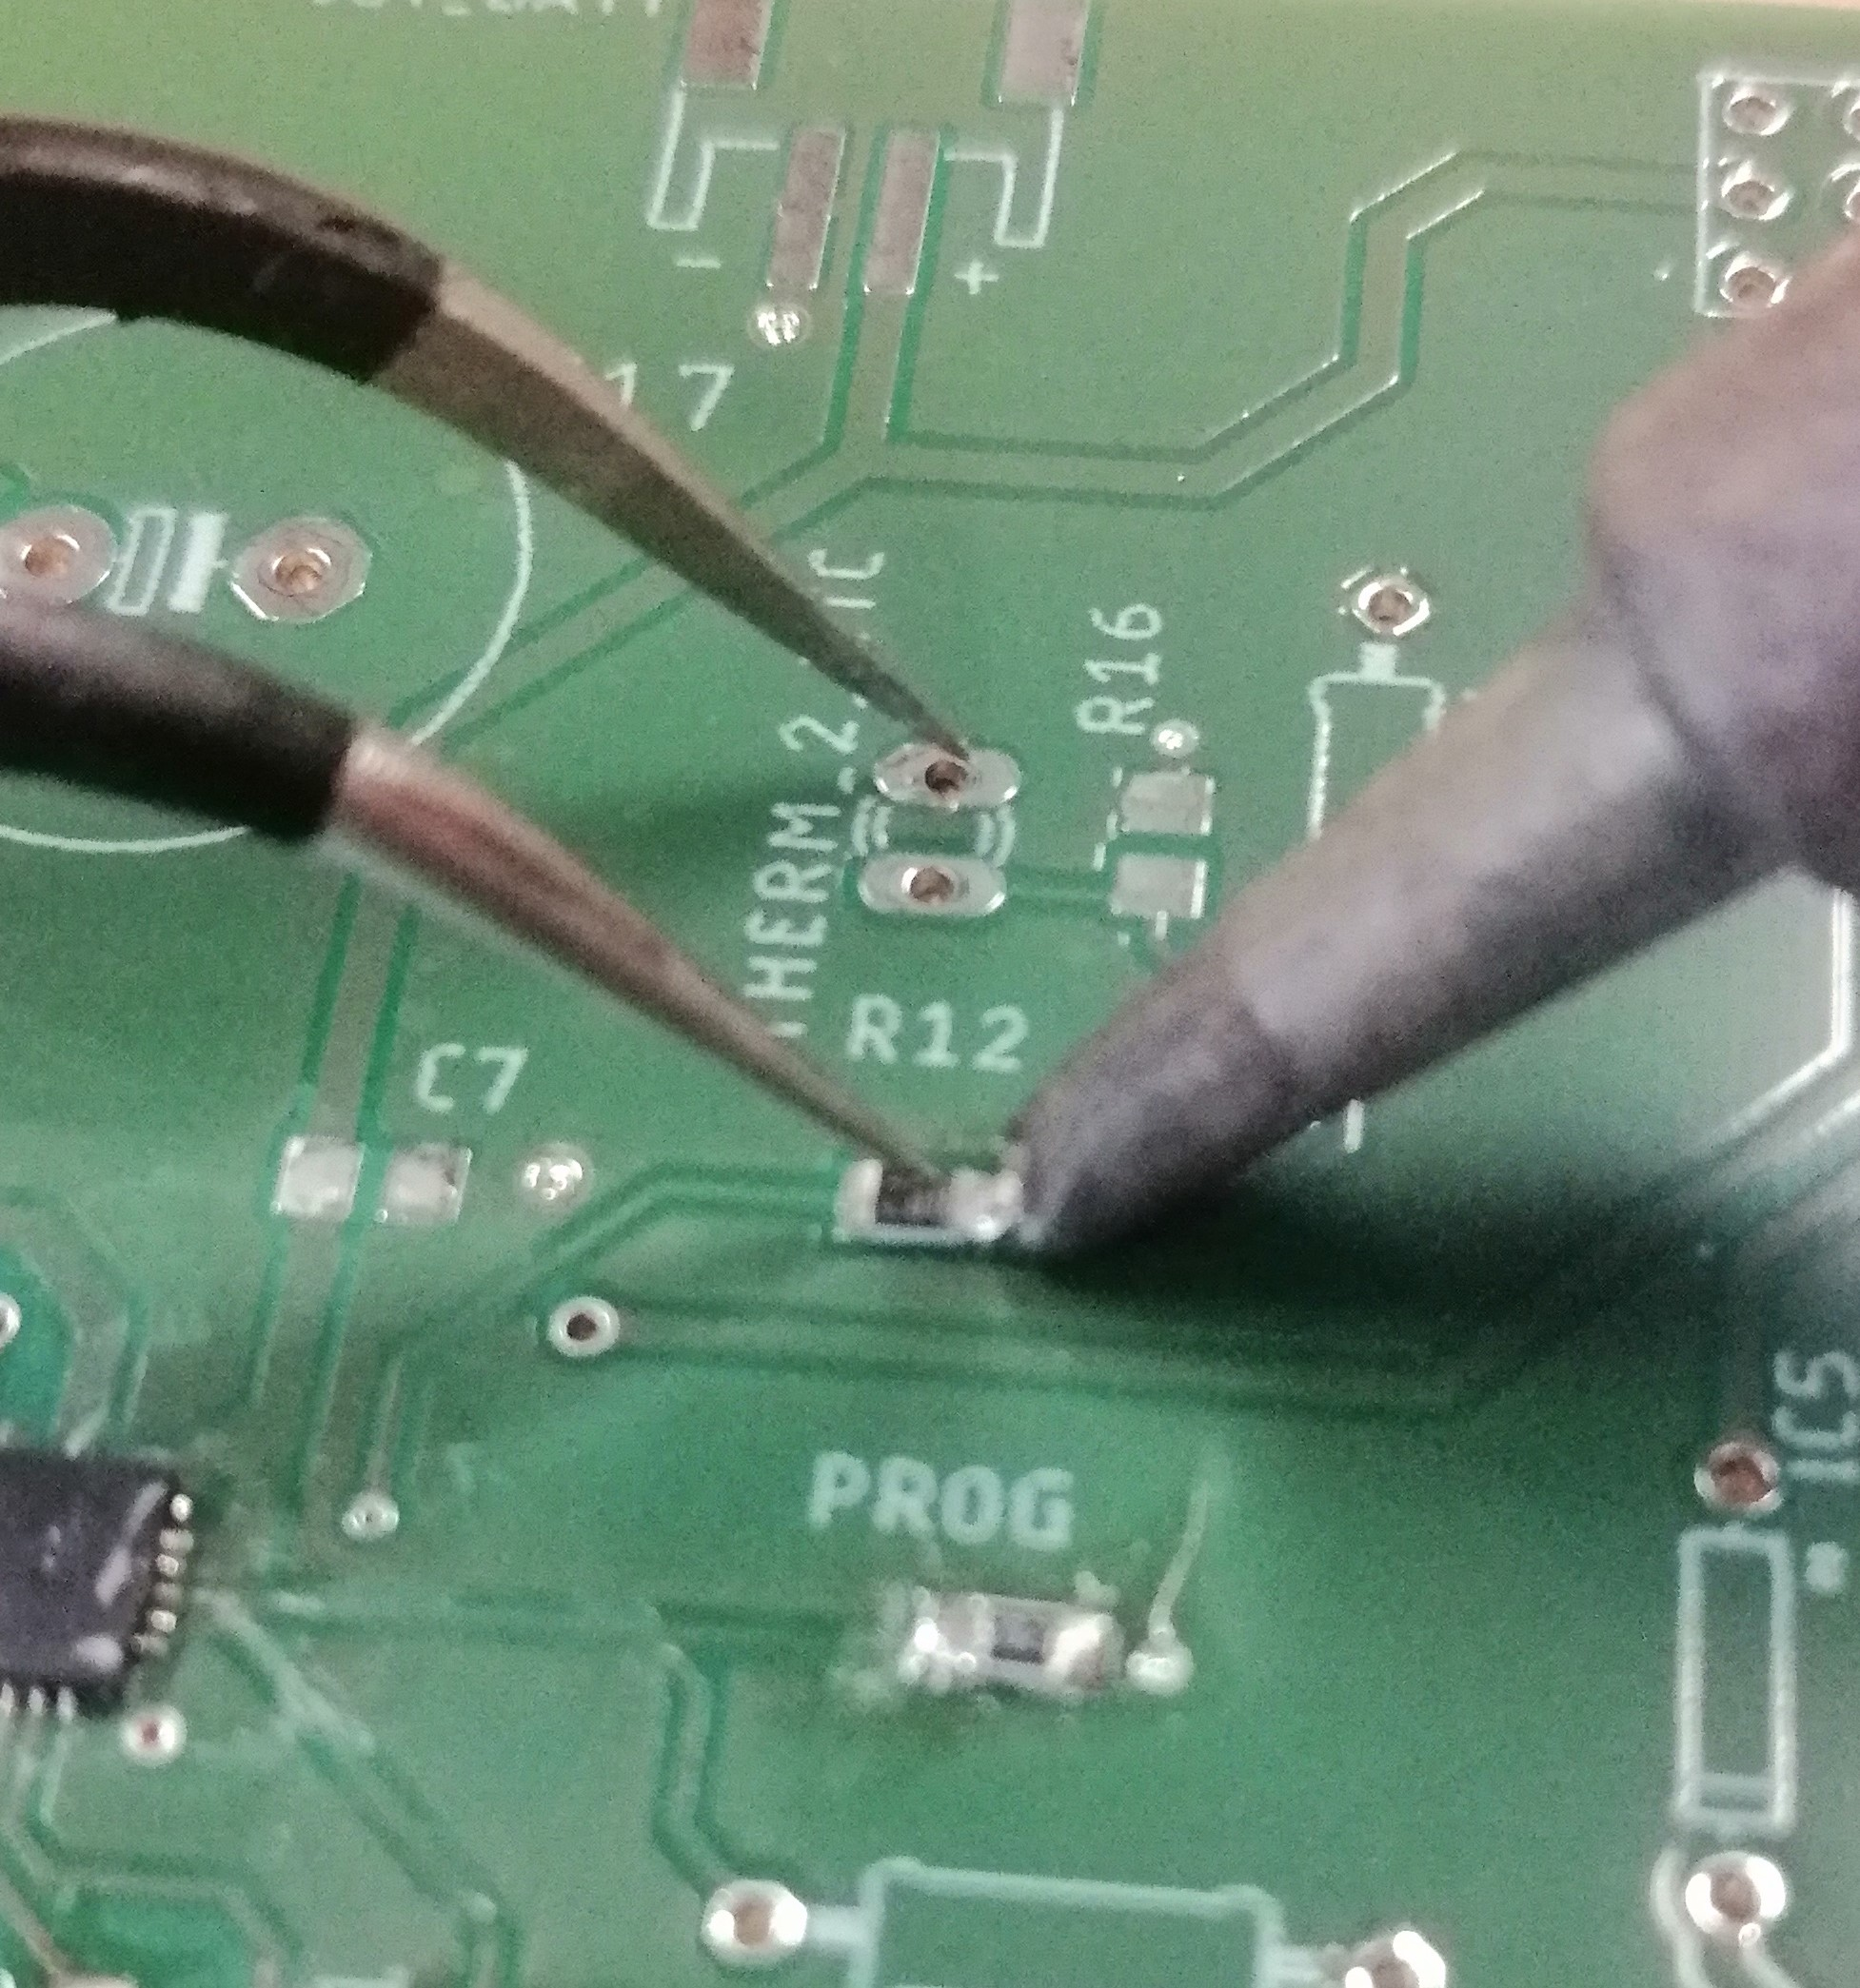
\includegraphics[width=0.8\linewidth]{graphics/HW_Val/SMD_Loeten.jpg}
\captionof{figure}{Das Löten eines SMD-Bauteils.}
\label{fig:SMD_Loeten}
\end{minipage}}


Die MCU hat ein TQFP gehäuse mit insgesamt 100 Pins (25 je Seite). Diese Pins sind äusserst nahe beieinander und sehr dünn, weshalb ein normales anlöten wie bei oben genannten SMD Bauteilen nicht gut funktioniert. Hier wird das oft \textit{Ziehlöten} genannte Verfahren angewendet. Dabei wird die MCU erst äusserst sorgfältig korrekt platziert. Mit einer Pinzette wird die MCU an Ort und Stelle gehalten. Die Pins auf einer Seite werden nun grosszügig mit Flussmittel eingestrichen. Direkt nach dem Einstreichen muss der Lötstab mit dem breiten Lötaufsatz und ganz wenig Lötzinn über die Pins fahren, um den Lötzinn auf die Pins zu verteilen. Nun kann wieder mit dem Flussmittel gearbeitet werden, wobei der Lötstab frontal von den Enden der Pins (MCU-seitig) nach aussen gzogen wird. Lötzinn muss im zweiten Schritt meistens keiner mehr verwendet werden und wenn doch, dann nur äusserst wenig. Die Kunst besteht darin, nicht zu viel Lötzinn zu verwenden, da sonst Lötbrücken entstehen können, welche nicht ganz einfach zu entfernen sind. Dieses Verfahren wird in Abbildung \todo[inline]{ref Bild einfügen MCU löten} dargestellt.

\subsubsection{Mängel der Erstversion und dessen Verbesserungen}
Die Mängel der Erstversion werden hier aufgelistet und deren Verbesserung für die Zweitversion direkt erläutert.
\begin{enumerate}
\item Beim ersten Testen des Boards wurde erkannt, dass Probleme mit dem Versorgungslayer bestehen, da fast alle Bauteile, welche mit diesem über ein Via (ein Verbinder zwischen Layer) verbunden sein sollten, nicht mit Strom versorgt wurden. Dieses Manko wurde provisorisch mit einer Leiterplatte und Drähten gelöst, so dass weitere Tests gemacht werden konnten.\\
Für die Zweitversion wurde die Füllung des Versorgungslayers mit direkten Leiterbahnen zu den entsprechenden Pins ersetzt.
\item In einem weiteren Schritt wurde erkannt, dass die ChargePump nicht die gewünschte Spannung ausgibt wie auf einem Steckbrett zuvor getestet, wobei sich dieser Mangel erst bei geringerem Akkustand bemerkbar macht, weshalb weitere Tests gemacht werden konnten.\\
Um dieses Problem zu beheben, sollen andere Dioden verwendbar sein, Aus diesem Grund werden für den zweiten Print THT-Bauteile verwendet, da diese einfacher auszulöten und zu ersetzen sind.
\item Gemäss den Tests sperren die Schutzdioden in der Nähe des DCIN Jacks nicht wie gewünscht in Sperrrichtung.\\
Auch hier werden für den zweiten Print THT-Bauteile verwendet, um ein austauschen der Dioden vornehmen zu können.
\item Pins für die serielle Schnittstelle (TXD und RXD) wurden vertauscht, weshalb keine Kommunikation über PuTTY erfolgen konnte.\\
Dieses Problem wurde im Redesign behoben, indem die Anschlüsse vertauscht wurden.
\item Beim SIM808 muss der Pin PWRKEY auf Ground sein um diesen starten zu können. Dieser Pin war jedoch nicht auf Ground gezogen sondern floating.\\
Der entsprechende Pin wurde im Redesign mit Ground verbunden.
\item Desweiteren konnte beim SIM808 die 1.8V Ausgangsspannung für die SIM-Karte nicht gemessen werden. Es wurde vermutet, dass es wegen des TVS-Arrays nicht möglich war. Für das TVS-Array wurde ein zu kleiner Footprint verwendet, weshalb die Lötaugen nicht zur Grösse des Gehäuses passte, was schliesslich zu defekten auf dem PCB führte.\\
Der Footprint wurde von Hand angepasst, so dass das Bauteil nun richtig angelötet werden kann. Ausserdem wurde eine Bestückungsvariante implementiert, mit der der SIM808 mit Breakout Board direkt angeschlossen werden kann über Pinheader.
\item Die Signale des Anemometers und des Ombrometers waren verrauscht, was auf einen ineffektiven Tiefpass hindeutet. Die Abstände zwischen Widerstand und Kondensator waren wirklich etwas weit entfernt.\\
Die Abstände wurden im Redesign massiv verringert.
\item Der verwendete Kippschalter trennt die Wetterstation von der Versorgung, jedoch ist der SIM808 direkt vom Akku gespiesen und läuft deshalb weiter.\\
Durch das Ersetzen des Kippschalters mit einem anderen, welcher 2 Stromkreise gleichzeitig schaltet, konnte dieses Problem im Redesign behoben werden.
\end{enumerate}
Die Mängel wurden gemäss den Erläuterungen behoben und ein zweites PCB bestellt. Das eingetroffene PCB wies weiterhin Problem 1 auf, was erst zu Ratlosigkeit führte. Schnell konnte jedoch herausgefunden werden, dass der Hersteller des PCBs (JLCPCB) keine Blind Vias unterstützt, welche jedoch für die Verbindung zwischen Bauteil und Versorgungslayer im Design verwendet wurden. Es musste deshalb ein drittes PCB bei einem Hersteller bestellt werden, welches Blind Vias unterstützt. Auf der Webseite www.multi-circuit-boards.eu konnten Blind Vias als Option angekreuzt werden, weshalb bei diesem Hersteller das dritte PCB bestellt wurde. Bestellen musste dies jedoch die FHNW, da dieser Anbieter nur an Institutionen und Unternehmen liefert und die Projektteilnehmer die kosten eines PCBs von rund 280.- nicht auf sich nehmen konnten. \\[0.5cm]
Das erfolgreich erhaltene dritte PCB wurde wie erläutert bestückt und getestet gemäss den dokumentierten Tests in Kapitel \ref{subsubsec:HW_Val}. Die Firmware konnte ebenso auf die MCU geflasht werden und funktioniert gemäss. \todo[inline]{Referenz zum Kapitel Firmwareverifikation} Die Wetterstation funktioniert soweit und benötigt lediglich ein Gehäuse, um präsentabel zu sein und um ein Betrieb im Freien zu ermöglichen. Auf diese Thematik wird im nächsten Kapitel eingegangen.

\subsection{Das Gehäuse}
\label{subsec:HW:Gehaeuse}
Damit die Wetterstation gebraucht werden kann, muss das PCB vor den Wettereinflüssen geschützt werden. In Absprache mit dem Auftraggeber soll als Wunschziel ein provisorisches Design des Gehäuses erfolgen und dieses mit einem 3D-Drucker gedruckt werden um bei der Bachelor-Thesis Ausstellung am 16. August 2019 ein anschauliches Modell zu haben. Im folgenden Unterkapitel wird aufgezeigt, auf was beim Design des Gehäuses acht gegeben werden muss und in einem folgenden Unterkapitel wird das Design für das provisorische Gehäuse vorgestellt.

\subsubsection{Wichtige Merkmale}
Damit beim Design des Gehäuses nichts vergessen geht, werden hier die wichtigsten Punkte, auf die acht gegeben werden muss, erläutert. Die grobe Dimensionierung wird durch das PCB vorgegeben und ist in Abbildung \ref{fig:Dimensionen1} zu sehen.

\begin{figure}[h]
\centering
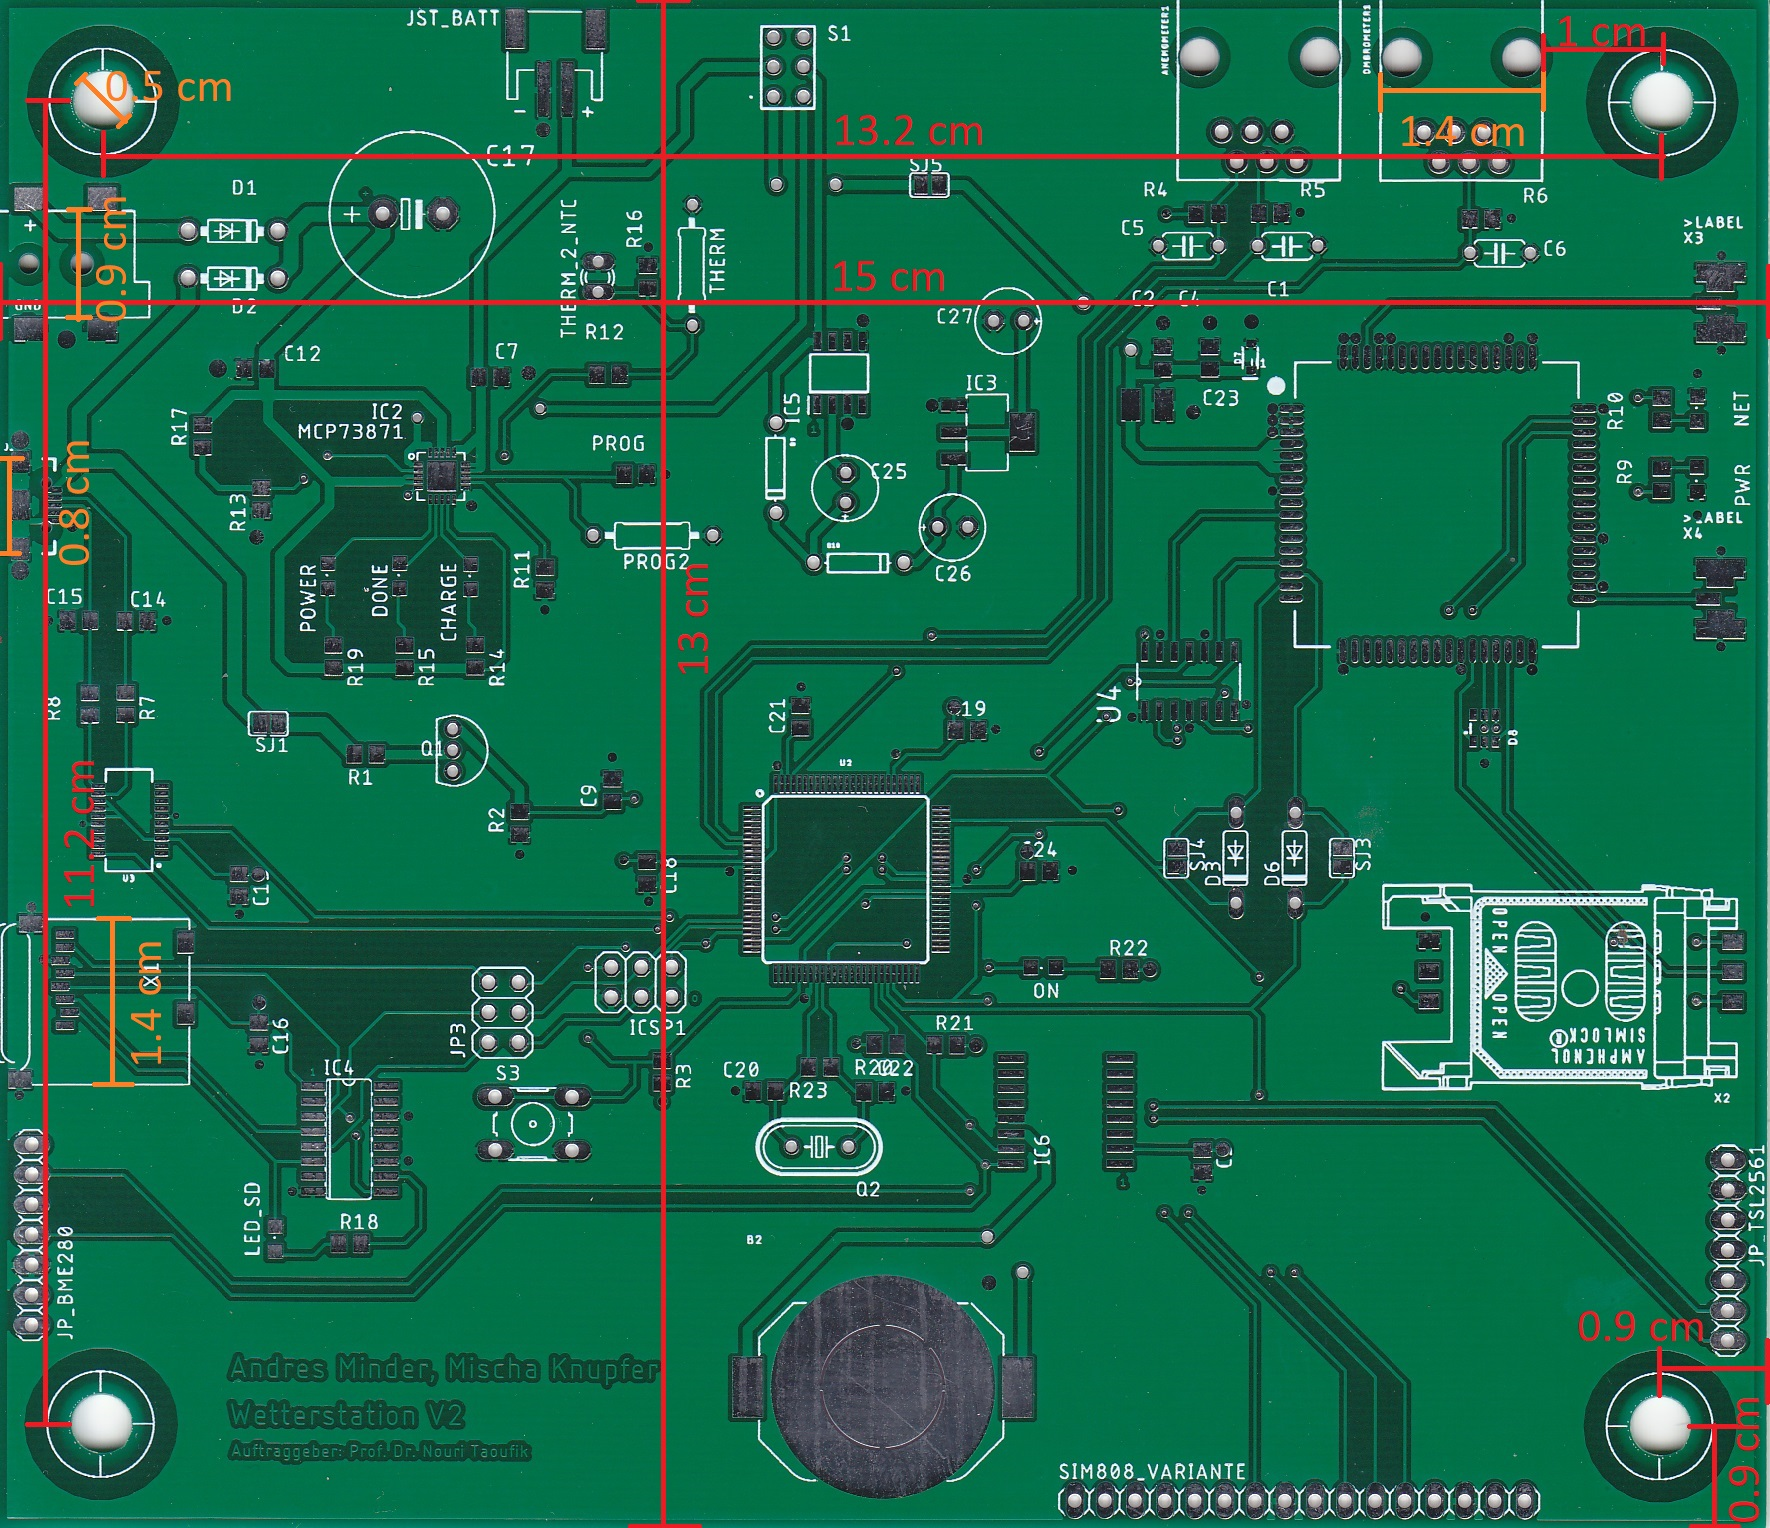
\includegraphics[width=0.9\linewidth]{graphics/Gehaeuse/PCB_Dimensionen.jpg}
\caption{Das noch unbestückte PCB mit den wichtigsten Dimensionen.}
\label{fig:Dimensionen1}
\end{figure}
\newpage
Abbildung \ref{fig:Dimensionen1} zeigt das noch unbestückte PCB, wie es schon in der Hardware Übersicht verwendet wurde, mit den wichtigsten Dimensionen. Das PCB hat eine Breite von 15cm, eine länge von 13cm. Die Mittelpunkte der 5mm breiten Bohrlöcher sind 13.2cm weit entfernt in der Breite und 11.2cm in der Länge, wobei diese jeweils 9mm vom Rand entfernt sind. Die Breite der Bauteile die aus dem Gehäuse hinausragen sind 1.4cm (RJ11, $\mu$SD), 0.9cm (DCIN Jack) und 0.8cm ($\mu$USB). Damit alle Bauteile von der Höhe her Platz haben, muss das Gehäuse nach oben hin mindestens über 3cm Freiraum verfügen wegen dem zum MCP73871 gehörenden Elektroly-Kondensator (C17). Der Akkumulator soll ebenfalls im Gehäuse Platz finden, weshalb genügend Platz (min. 2cm) in der Tiefe für diesen zur Verfügung stehen muss. Da es eine Bestückungsvariante gibt für den SIM808, soll das Gehäuse an der unteren Seite um mindestens 4cm erweitert werden, da das Breakout Board des SIM808 ansonsten nicht angeschlossen werden kann. Auf der rechten Seite werden Antennen für den SIM808 angeschlossen, weshalb das Gehäuse auf dieser Seite um mindestens 1cm erweitert werden soll, damit diese nicht knicken. Ebenfalls sollen auch die Kabel des Akkumulators vom knicken geschützt werden, hier benötigt man eine erweiterung des Gehäuses von mindestens 3mm, da die Kabel selbst eine höhere Flexibilität als die Antennen aufweisen. Auf der linken Seite befindet sich die $\mu$USB-Buchse, sowie die Öffnung für die $\mu$SD-Karte. Diese Öffnungen ragen ein wenig hinaus und sollten gut geschützt werden, weshalb eine Erweiterung der Dimensionierung auf der Linken Seite von 1mm empfohlen ist. Äusserst wichtig ist ebenfalls, dass der BME280 auf der linken Seite des Gehäuses nach aussen gebracht wird und in einem gut mit Aussenluft durchströmten eigenen Raum seinen Platz findet. Der TSL2561 wird ebenfalls auf der rechten Seite nach aussen geführt, damit dieser dort unter einem mit durchsichtigem Plexiglas versehenen eigenen Raum die Lichtintensität messen kann.\\[0.5cm]
Die wichtigsten Punkte wurden erläutert, weshalb es nun zum Design des Gehäuses kommt, welches im nächsten Abschnitt vorgestellt wird.

\subsubsection{Das Design}
Im vorhergehenden Unterkapitel wurden die wichtigsten Merkmale und Dimensionen des Gehäuses erläutert. In diesem Unterkapitel wird nun das provisorische Design vorgestellt. Da für den Zusammenbau das PCB auf einen Teil des Gehäuses gelegt wird und mit einem zweiten Teil überdeckt, wird in diesem Abschnitt der Begriff \textit{Boden} für den unteren Teil und \textit{Deckel} für den oberen Teil verwendet. Das Design wurde mit dem CAD-Programm Autodesk Fusion 360 erstellt, welches den Studenten von Bildungseinrichtungen wie der FHNW frei zur Verfügung steht.
\newpage

\begin{figure}[h]
\centering
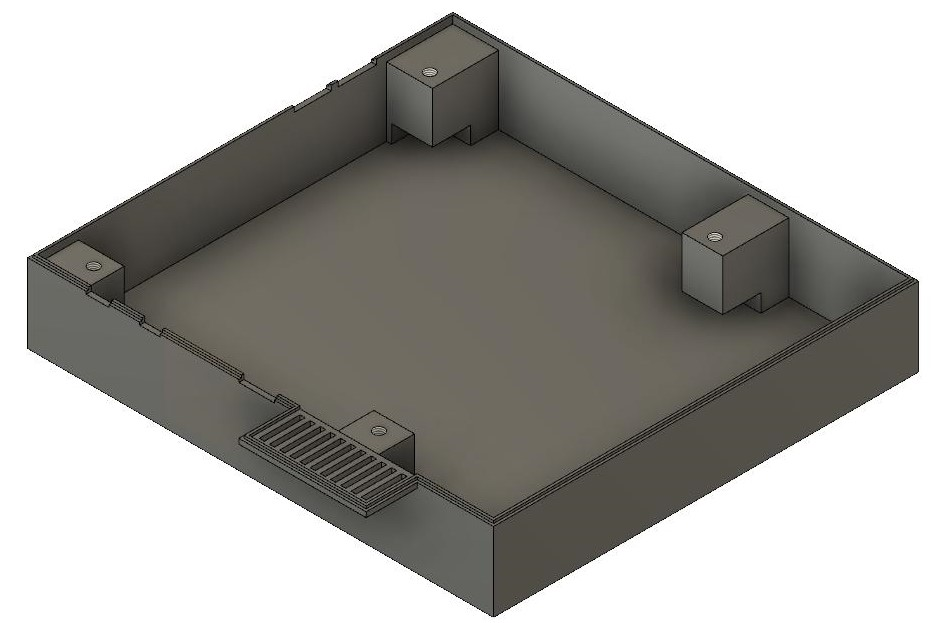
\includegraphics[width=0.99\linewidth]{graphics/Gehaeuse/Design_Boden.jpg}
\caption{Gesamtansicht des Designs des Bodens.}
\label{fig:D:Boden}
\end{figure}

Die Gesamtansicht des Designs des Bodens ist in Abbildung \ref{fig:D:Boden} zu sehen. Diverse Blöcke und Aussparungen sind deutlich zu sehen, worauf mit der Hilfe von den nachfolgenden Abbildungen näher eingegangen wird.\\

{\begin{minipage}[b][8cm][t]{0.39\textwidth}
Das PCB muss erhöht sein, damit der Akku darunter Platz findet. Ausserdem soll eine Schraube das Gehäuse mit dem PCB verbinden. Aus diesen Gründen wurden im Boden Blöcke implementiert, welche ein Schraubengewinde besitzen, wie in Abbildung \ref{fig:D:Boden:Schrauben} ersichtlich ist. Am unteren Ende des Schraubenblocks befindet sich eine Aussparung. Diese Aussparung bietet Platz für eine Mutter, falls das implementierte Gewinde fehlerhaft gedruckt wird.
\end{minipage}}
{\begin{minipage}[b][8cm][t]{0.6\textwidth}
\centering
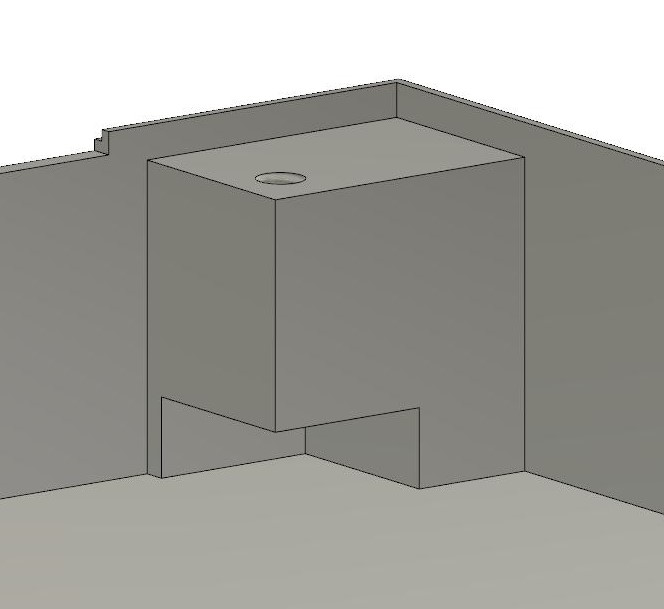
\includegraphics[width=0.8\linewidth]{graphics/Gehaeuse/Design_Boden_Schrauben.jpg}
\captionof{figure}{Design des Schraubenblocks des Bodens.}
\label{fig:D:Boden:Schrauben}
\end{minipage}}

\newpage
\begin{figure}[h]
\centering
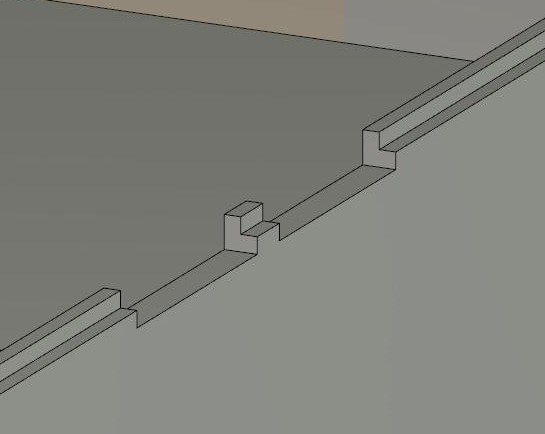
\includegraphics[width=0.5\linewidth]{graphics/Gehaeuse/Design_Boden_Aussparungen.jpg}
\caption{Aussparungen für Bauteile, welche aus dem Gehäuse hinausragen.}
\label{fig:D:Boden:Aussparungen}
\end{figure}
Die in Abbildung \ref{fig:D:Boden:Aussparungen} ersichtlichen Aussparungen sind notwendig um Öffnungen im Gehäuse zu generieren, welche Platz für die hinausragenden Bauteile bieten. Beim Boden sind diese Aussparungen alle gleich tief, da die Bauteile alle auf dem planen PCB angelötet sind und dieses somit als Referenz gilt.

\begin{figure}[h]
\centering
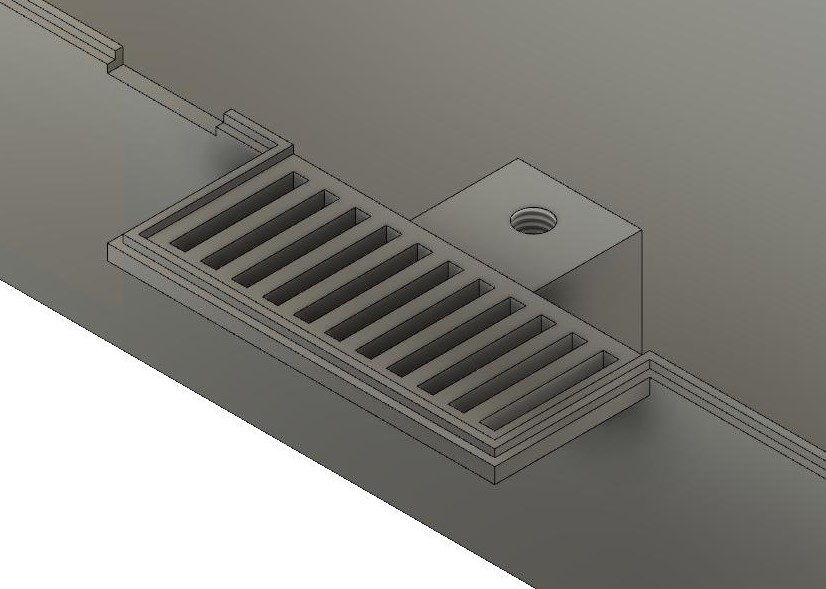
\includegraphics[width=0.7\linewidth]{graphics/Gehaeuse/Design_Boden_BME.jpg}
\caption{Seitenwand für den BME280-Extraraum mit Luftschlitzen.}
\label{fig:D:Boden:BME}
\end{figure}
Der BME280 muss nach aussen geführt werden in einen kleinen Extraraum, welcher gut belüftet ist. Nur so ist der BME280 in der Lage, die exakten Messwerte liefern zu können. Aus diesem Grund wird ein kleiner Extraraum am Rand des Gehäuses gefertigt, welcher mit Luftschlitzen versehen ist. In Abbildung \ref{fig:D:Boden:BME} sieht man den Boden für den im Deckel implementierten Extraraum. Der Boden ist, wie erwähnt, mit 2mm breiten Luftschlitzen versehen.

\newpage

\begin{figure}[h]
\centering
\includegraphics[width=0.99\linewidth]{graphics/Gehaeuse/Design_Deckel.jpg}
\caption{Gesamtansicht des Designs des Deckels.}
\label{fig:D:Deckel}
\end{figure}
Die Gesamtansicht des Designs des Deckels ist in Abbildung \ref{fig:D:Deckel} zu sehen. Wie schon beim Boden sind auch hier diverse Blöcke und Aussparungen zu sehen, auf welche mit der Hilfe von den nachfolgenden Abbildungen näher eingegangen wird.\\

{\begin{minipage}[b][9cm][t]{0.39\textwidth}
Die Schraubenblöcke des Deckels sind weniger interessant, da diese durchgehende Blöcke sind mit einem entsprechenden Gewinde. Aus diesem Grund wurde in Abbildung \ref{fig:D:Deckel:Schrauben} die Aussenseite des Deckels abgebildet, welche die Schraubenversenkung zeigt. In dieser Schraubenversenkung wird der Kopf der verwendeten Schraube seinen Platz finden, weshalb es zu keinem herausragen einer Schraube kommt.
\end{minipage}}
{\begin{minipage}[b][9cm][t]{0.6\textwidth}
\centering
\includegraphics[width=0.8\linewidth]{graphics/Gehaeuse/Design_Deckel_Schraubenversenkung.jpg}
\captionof{figure}{Schraubenversenkung im Deckel.}
\label{fig:D:Deckel:Schrauben}
\end{minipage}

\begin{figure}[h]
\centering
\includegraphics[width=0.6\linewidth]{graphics/Gehaeuse/Design_Deckel_BMEundAussparungen.jpg}
\caption{Aussparungen für Bauteile, welche aus dem Gehäuse hinausragen und der designte Extraraum für den BME280 mit Luftschlitzen.}
\label{fig:D:Deckel:BME}
\end{figure}
Abbildung \ref{fig:D:Deckel:BME} zeigt den bereits erwähnten Extraraum des BME280. Die Luftschlitze sind deutlich zu erkennen und an jeder Seite des Extraraumes angebracht. Ausserdem ist auf dieser Abbildung ebenso ersichtlich, dass die Aussparungen verschiedene Höhen aufweisen. Die Höhe einer Aussparung ist Bauteilabhängig, genauso wie deren Breite.

\begin{figure}[h]
\centering
\includegraphics[width=0.5\linewidth]{graphics/Gehaeuse/Design_Deckel_TSL.jpg}
\caption{Öffnung und Bohrungen für den TSL2561 und den BME280.}
\label{fig:D:Deckel:TSL}
\end{figure}
Um den BME280 und den TSL2561 hinausführen zu können, wurden im Gehäuse entsprechende Öffnungen und auch Schraubenlöcher eingelassen. Die eben genannten Öffnungen und Schraubenlöcher sind in Abbildung \ref{fig:D:Deckel:TSL} äusserst gut ersichtlich.
\newpage
{\begin{minipage}[b][6cm][t]{0.49\textwidth}
\centering
\includegraphics[width=0.8\linewidth]{graphics/Gehaeuse/Design_Boden_Rand.jpg}
\captionof{figure}{Design des Randes vom Boden zum Deckel hin.}
\label{fig:D:Boden:Rand}
\end{minipage}}
{\begin{minipage}[b][6cm][t]{0.49\textwidth}
\centering
\includegraphics[width=0.8\linewidth]{graphics/Gehaeuse/Design_Deckel_Rand.jpg}
\captionof{figure}{Design des Randes vom Deckel zum Boden hin.}
\label{fig:D:Deckel:Rand}
\end{minipage}}

Damit das Befestigen des Bodens mit dem Deckel einfacher zu handhaben ist, wurde beim Boden die äussere Hälfte des Randes um 1mm gesenkt, wobei beim Deckel die innere Hälfte des Randes um 1mm gesenkt wurde. Dank diesem Feature ist es möglich den Deckel wie ein Puzzlestück am Boden anzubringen, bevor die Verschraubung von statten geht.\\[0.25cm]
Das Design des Gehäuses für das PCB wurde in diesem Unterkapitel näher erläutert. Es sei jedoch erwähnt, dass dieses Gehäuse nicht geeignet ist um die Wetterstation im freien betreiben zu können. Das hier vorgestellte Design zeigt lediglich auf, auf was beim Gehäuse, in Bezug auf das PCB, geachtet werden muss. Damit das Gehäuse für den Gebrauch im freien taugt, muss es zwingend gegen Regen und Staub dicht sein, so dass die verwendete Elektronik keine Schäden erleidet. Dennoch muss der BME280 mit Aussenluft belüftet werden, was bei einem möglichst Regen- und Staubdichten Gehäuse eine zusätzliche, kontrollierte Belüftung notwendig macht. Ausserdem muss auf einen möglichen Hitzestau durch Sonneneinstrahlung getestet und gegebenfalls eine Kühlung integriert werden.

\subsubsection{Probleme mit dem gedruckten Gehäuse}
Das mit einem 3D-Printer gedruckte Gehäuse aus weissem PLA weist Mängel auf. Zum einen kam es durch die Schwingungen des Druckers zu Fehlprints im Bereich des Extraraumes für den BME280, da die Lamellen zu instabil sind (dünn und lang). Das implementierte Gewinde für die Schrauben war unzureichend gedruckt, weshalb es lediglich zu einer Verengung des Schraubenlochs kam und kleinere Schrauben verwendet werden mussten. Zudem hin kommt eine Differenz in der Distanz der Bohrlöcher, denn die Bohrlöcher scheinen wegen 1mm nicht aufeinander zu passen und mussten deshalb aufgebohrt werden. Dies führte dazu, dass am unteren Ende für die Schrauben eine Mutter positioniert und angeklebt werden musste, da die Schrauben sonst keinen Halt fänden. Ebenfalls gab es Probleme beim BME280 und beim TSL2561, weil die auf dem Print implementierten Pinheader mit den Schraubenblocks kollidierten, was ebenfalls mit einer Bohrmaschine behoben wurde. Die Anschlüsse auf der Seite des $\mu$USB-Anschlusses ragten nicht hinaus, weshalb die Öffnung des $\mu$USB-Anschlusses vergrössert werden musste, damit ein Kabel angeschlossen werden kann. Die Schrauben, um den BME280 und den TSL2561 zu befestigen, gab es im OBI nicht zu kaufen, weshalb auf Holzschrauben mit angemessenem Durchmesser zurückgegriffen werden musste und eine Holzleiste für die Befestigung benötigt wurde. Der transparente Raum für den TSL2561 konnte nicht gedruckt werden, da das transparente Filament nicht transparent genug wäre und Rillen enthalten würde, weshalb ein transparentes Stück Plastik einer Verpackung angeklebt wurde. \\[0.25cm]
Die Firmware, die Hardware und das Gehäuse wurden erstellt, weshalb nun die Validierung des Konzepts im nächsten Kapitel folgt.


\cleardoublepage
\thispagestyle{empty}
\vspace*{4cm}
\begin{center}
	\section{Abschluss}
	\label{sec:Abschluss}
\end{center}
\newpage
\subsection{Konzeptvalidierung}
\label{subsec:Konzeptvalidierung}

\subsubsection{Validierung der Hardware}
\label{subsubsec:HW_Val}
Die Validierung der Hardware ist ein wichtiger Schritt um Denk- und Designfehler zu entdecken bzw. den geplanten Betrieb der Hardware sicherzustellen. Aus diesem Grund wird in diesem Unterkapitel die Validierung der Hardware thematisiert und mit Abbildungen anschaulich dargestellt. Bevor jedoch die Validierung von statten geht, werden die verwendeten Gerätschaften im nächsten Abschnitt kurz erläutert.\\
\paragraph{\textbf{Verwendete Gerätschaften}}[0.4cm]
{\begin{minipage}[b][9cm][t]{0.42\textwidth}
Damit die Hardware validiert werden kann, braucht es spezielle Geräte. Zum einen wird ein FLUKE 117 (Abbildung \ref{fig:FLUKE}), ein handliches RMS Multimeter, benutzt. Zwei Hauptfunktionen des FLUKEs werden hauptsächlich verwendet, diese sind das Messen von Gleichspannung, sowie die Messgerätfunktion Kontinuität, um zu testen ob elektrische Verbindungen bestehen \cite{FLUKE}. Zum anderen wird der TDS 210, ein Digitales Real-Time Oszilloskop von Tektronix, verwendet, um Spannungsverläufe zu analysieren. In Abbildung \ref{fig:KO} ist dieser zu sehen. Um genaue Eingangsspannungen generieren zu können, wird ein Speisegerät verwendet, welches in der Abbildung \ref{fig:PowerSupply} zu sehen ist.
\end{minipage}}
{\begin{minipage}[b][9cm][t]{0.57\textwidth}
\centering
\includegraphics[width=0.6\linewidth]{graphics/HW_Val/Fluke.jpg}
\captionof{figure}{Das handliche RMS Multimeter FLUKE 117 mit Sonden.}
\label{fig:FLUKE}
\end{minipage}}

{\begin{minipage}[b][7cm][t]{0.49\textwidth}
\centering
\includegraphics[width=0.9\linewidth]{graphics/HW_Val/KO.jpg}
\captionof{figure}{TDS 210 von Tektronix.}
\label{fig:KO}
\end{minipage}}
{\begin{minipage}[b][7cm][t]{0.49\textwidth}
\centering
\includegraphics[width=0.9\linewidth]{graphics/HW_Val/PowerSupply.jpg}
\captionof{figure}{Das verwendete Speisegerät.}
\label{fig:PowerSupply}
\end{minipage}}

Die Geräte wurden nun vorgestellt, weshalb im nächsten Abschnitt bereits mit der Validierung der Energieversorgung begonnen wird.
\newpage
\paragraph{\textbf{Validierung der Energieversorgung}}[0.4cm]
{\begin{minipage}[b][6.5cm][t]{0.42\textwidth}
Die Energieversorgung ist äusserst wichtig, da ohne eine funktionierende Energieversorgung kein Bauteil seiner Funktion nachgehen kann. Zuerst wird kontrolliert, ob die Verbindungen der Leiterbahnen für das 3.3V-Netz bestehen. Dies wird mit der Kontinuitätsfunktion (Abbildung \ref{fig:Kontinuitaet}) des Flukes gemacht, bei welcher ein Ton erklingt sobald eine elektrische Verbindung besteht (kleiner Widerstand). Es werden vom Ausgang des Linearreglers aus alle Verbindungen getestet, welche in Abbildung \ref{fig:Verbindungstestpunkte} eingezeichnet wurden.
\end{minipage}}
{\begin{minipage}[b][6.5cm][t]{0.57\textwidth}
\centering
\includegraphics[width=0.6\linewidth]{graphics/HW_Val/Kontinuitaet.jpg}
\captionof{figure}{Das Zeichen für die Kontinuitätsfunktion des FLUKEs.}
\label{fig:Kontinuitaet}
\end{minipage}}
\begin{figure}[h]
\centering
\includegraphics[width=0.9\linewidth]{graphics/HW_Val/Verbindungstestpunkte.jpg}
\caption{Die Rot markierten Stellen zeigen die Endpunkte des Verbindungstests an. Die Orange markierte Stelle zeigt den Startpunkt an.}
\label{fig:Verbindungstestpunkte}
\end{figure}

Die Verbindungen konnten erfolgreich verifiziert werden. Bei jedem Punkt gemäss Abbildung \ref{fig:Verbindungstestpunkte} ist ein Signalton aus dem FLUKE gekommen, was eine bestehende elektrische Verbindung signalisiert.

Als zweites wird nach dem Bestücken der Energieversorgung diese ausgetestet. Es wird überprüft, ob der Linearregler am Ausgang auf 3.3V regelt. Ausserdem muss überprüft werden, ob die ChargePump die Akkuspannung auf das gewünschte Potenzial bringt. Darüber hinaus muss noch getestet werden, ob die Dioden in der nähe des DCIN Jacks wie gewünscht in Sperrichtung sperren. Für diese Tests müssen Spannungsverläufe auf dem TDS 210 betrachtet werden, sowie mit dem Speisegerät eine Eingangsspannung erzeugt werden. Die nachfolgende Bilder zeigen jeweils die Testpunkte der Messung, sowie die Visualisierung der gemessenen Spannung auf dem TDS 210.\\[0.5cm]

{\begin{minipage}[b][8cm][t]{0.49\textwidth}
\centering
\includegraphics[width=0.9\linewidth]{graphics/HW_Val/Test_Eingangsspannung.jpg}
\captionof{figure}{Testpunkt zur Überprüfung der Eingangsspannung.}
\label{fig:Test_Eingangsspannung}
\end{minipage}}
{\begin{minipage}[b][8cm][t]{0.49\textwidth}
\centering
\includegraphics[width=0.9\linewidth]{graphics/HW_Val/Ergebnis_Eingangsspannung.jpg}
\captionof{figure}{Die Eingangsspannung auf dem TDS 210 visualisiert. Es werden 4V angezeigt.}
\label{fig:Ergebnis_Eingangsspannung}
\end{minipage}}

{\begin{minipage}[b][8cm][t]{0.49\textwidth}
\centering
\includegraphics[width=0.9\linewidth]{graphics/HW_Val/Test_ChargePump.jpg}
\captionof{figure}{Testpunkt um die Spannungserhöhung der ChargePump zu messen.}
\label{fig:Test_ChargePump}
\end{minipage}}
{\begin{minipage}[b][8cm][t]{0.49\textwidth}
\centering
\includegraphics[width=0.9\linewidth]{graphics/HW_Val/Ergebnis_ChargePump.jpg}
\captionof{figure}{Die durch die ChargePump erhöhte Spannung, welche auf dem TDS 210 visualisiert wurde. Es werden etwas mehr als 6V angezeigt.}
\label{fig:Ergebnis_ChargePump}
\end{minipage}}

{\begin{minipage}[b][8cm][t]{0.49\textwidth}
\centering
\includegraphics[width=0.9\linewidth]{graphics/HW_Val/Test_Ausgangsspannung.jpg}
\captionof{figure}{Testpunkt für die Ausgangsspannung des Linearreglers.}
\label{fig:Test_Ausgangsspannung}
\end{minipage}}
{\begin{minipage}[b][8cm][t]{0.49\textwidth}
\centering
\includegraphics[width=0.9\linewidth]{graphics/HW_Val/Ergebnis_Ausgangsspannung.jpg}
\captionof{figure}{Die durch den Linearregler geregelte Ausgangsspannung. Es werden rund 3.3V angezeigt.}
\label{fig:Ergebnis_Ausgangsspannung}
\end{minipage}}

Die Abbildungen \ref{fig:Test_Eingangsspannung}, \ref{fig:Test_ChargePump} und \ref{fig:Test_Ausgangsspannung} zeigen die Testpunkte, an denen gemessen wurde. Die Ergebnisse davon sind in den Abbildungen \ref{fig:Ergebnis_Eingangsspannung}, \ref{fig:Ergebnis_ChargePump} und \ref{fig:Ergebnis_Ausgangsspannung} zu sehen. Das Ergebnis der Eingangsspannung zeigt, dass kein Kurzschluss vorhanden ist und die Spannung vom Speisegerät her auf dem PCB ankommt. Gemäss dem Ergebnis der Messung der ChargePump stellt man fest, dass diese ebenfalls funktioniert und die Spannung deutlich erhöht. Der Linearregler erzeugt aus der Spannung der ChargePump die benötigten 3.3V, was dem Ergebnis dieser Messung zu entnehmen ist. Es kann gesagt werden, dass die Energieversorgung soweit funktioniert.
\todo[inline]{Wie niedrige Spannung noch funktionstauglich, messung mit solarpanel ebenfalls}

Versorgungstechnisch hat das PCB die Tests bestanden, weshalb nun mit dem Herzstück der Wetterstation, der MCU-Bauteilgruppe, fortgefahren wird.

\paragraph{\textbf{Validierung der MCU-Bauteilgruppe}}[0.2cm]
In einem weiteren Schritt wird die MCU mit ihrer Peripherie auf dem PCB angelötet. Um zu testen, ob die MCU funktioniert, wird diese über den ICSP-Header geflasht (über ein AVR-Dragon) und dabei auf einen externen 8MHz-Clock eingestellt. Die LED soll nach dem flashen zu Testzwecken blinken, da die MCU in betrieb ist. Ausserdem soll die LED nicht mehr leuchten, solange der Reset-Button gedrückt wird.

{\begin{minipage}[b][8cm][t]{0.49\textwidth}
\centering
\includegraphics[width=0.9\linewidth]{graphics/HW_Val/MCU_flashen.jpg}
\captionof{figure}{Verbindung zwischen AVR-Dragon und MCU.}
\label{fig:MCU_flashen}
\end{minipage}}
{\begin{minipage}[b][8cm][t]{0.49\textwidth}
\centering
\includegraphics[width=0.9\linewidth]{graphics/HW_Val/MCU_LED.jpg}
\captionof{figure}{Die leuchtende LED der MCU.}
\label{fig:MCU_LED}
\end{minipage}}

{\begin{minipage}[b][7cm][t]{0.49\textwidth}
Abbildung \ref{fig:MCU_flashen} zeigt, wie die MCU mit einem Programm geflasht wird, wobei ein AVR-Dragon verwendet wird, welcher am ICSP Header angeschlossen ist. Das Blinken der LED kann leider nicht mit Bildern festgehalten werden, jedoch kann mit Hilfe des TDS 210 auch dieser Signalverlauf angezeigt werden, wie in Abbildung \ref{fig:Blinken_LED} ersichtlich.
\end{minipage}}
{\begin{minipage}[b][7cm][t]{0.49\textwidth}
\centering
\includegraphics[width=0.9\linewidth]{graphics/HW_Val/Blinken_LED.jpg}
\captionof{figure}{Signalverlauf der blinkenden LED.}
\label{fig:Blinken_LED}
\end{minipage}}

{\begin{minipage}[b][7cm][t]{0.49\textwidth}
\centering
\includegraphics[width=0.9\linewidth]{graphics/HW_Val/Testpunkt_Quarz.jpg}
\captionof{figure}{Messung am Quarz.}
\label{fig:Testpunkt_Quarz}
\end{minipage}}
{\begin{minipage}[b][7cm][t]{0.49\textwidth}
\centering
\includegraphics[width=0.9\linewidth]{graphics/HW_Val/Ergebnis_Quarz.jpg}
\captionof{figure}{Das oszillierende Signal des Quarzes auf dem TDS 210.}
\label{fig:Ergebnis_Quarz}
\end{minipage}}

An welcher Stelle der Quarz getestet wurde, ist in Abbildung \ref{fig:Testpunkt_Quarz} ersichtlich. Das Ergebnis kann in Abbildung \ref{fig:Ergebnis_Quarz} betrachtet werden. Es ist zu sehen, dass der Quarz mit den gewünschten 8MHz schwingt.

Da die MCU-Bauteilgruppe nun getestet wurde, wird als nächstes die serielle Schnittstelle ($\mu$USB-Anschluss) validiert, um weitere Bauteilgruppen mit dessen Hilfe validieren zu können.

\paragraph{\textbf{Validierung der seriellen Schnittstelle}}[0.2cm]
Die Bauteilgruppe der seriellen Schnittstelle wird nun auf dem PCB angelötet. Deren Funktion wird mit Hilfe eines Programms auf der MCU und PuTTY (ein Emulator für serielle Schnittstellen auf dem Computer) getestet.

{\begin{minipage}[b][7.5cm][t]{0.49\textwidth}
\centering
\includegraphics[width=0.9\linewidth]{graphics/HW_Val/Testpunkt_serial.jpg}
\captionof{figure}{Messung an einem Via der TRX-Signalbahn der MCU.}
\label{fig:Testpunkt_serial}
\end{minipage}}
{\begin{minipage}[b][7.5cm][t]{0.49\textwidth}
\centering
\includegraphics[width=0.9\linewidth]{graphics/HW_Val/Ergebnis_serial.jpg}
\captionof{figure}{Signalverlauf der von der MCU gesendeten Zeichen.}
\label{fig:Ergebnis_serial}
\end{minipage}}\\
Die Abbildungen \ref{fig:Testpunkt_serial} und \ref{fig:Ergebnis_serial} zeigen den Ort des gemessenen Signals und dessen Verlauf. Es ist ersichtlich, dass die gesendeten Zeichen von der MCU aus auf den FT231XS gelangen. Der Ausgang des FT231XS wird über die $\mu$USB-Schnittstelle an das Notebook gesendet und dort mit Hilfe von PuTTY auf dem Bildschirm sichtbar.

Daten können über die serielle Schnittstelle übertragen werden, womit im folgenden Abschnitt auf die Validierung der Datenspeicherung eingegangen werden kann.

\paragraph{\textbf{Validierung der Datenspeicherung}}[0.2cm]
Bei der Bauteilgruppe der Datenspeicherung wird mit Hilfe der seriellen Schnittstelle die Funktionsweise getestet. Dies geschieht, indem ein File auf der $\mu$SD-Karte gespeichert und über die serielle Schnittstelle ausgelesen wird.


Die Datenspeicherung wurde erfolgfreich validiert, weshalb im nächsten Abschnitt auf die etwas grössere Bauteilgruppe des SIM808 eingegangen wird.

\paragraph{\textbf{Validierung des SIM808}}[0.2cm]
Als nächster grosser Schritt wird die SIM808 mit deren Peripherie implementiert. Es wird getestet, ob die SIM-Karte eine 1.8V Speisung erhält (einfache Spannungsmessung). Nachfolgend wird dann das Senden und Empfangen einer SMS, sowie das ermitteln des Standorts über ein kleines Testprogramm getestet. Die LEDs werden dabei auf ihr korrektes Verhalten hin beobachtet. 

\todo[inline]{Fazit SIM808test}

Es wurden bereits einige Bauteilgruppen validiert, jedoch bleiben unter anderem die RTC, das Ombrometer, das Anemometer und der Windrichtungsgeber, weshalb im nächsten Abschnitt darauf eingegangen wird.

\paragraph{\textbf{Validierung der Peripherie und der RTC}}[0.2cm]
Nun werden die RTC, das Ombrometer und das Anemometer mit Windrichtungsgeber angeschlossen. Die Signale des Ombrometers, des Anemometers und des Windrichtungsgebers werden auf ein möglichst sauberes (unverrauschtes) Signal hin getestet und die Flanken des Ombrometers und des Anemometers auf Störungen untersucht. Die Flanke sollte gemäss Abbildung \ref{fig:Flankenbeispiel}, stetig steigend, aussehen, sodass keine Mehrfachdetektionen wegen Störungen auftreten.

\todo[inline]{Fazit RTC Anemo Ombro test}

Nun bleiben nur noch der BME280 und der TSL2561 offen für die Validierung, weshalb im nächsten Abschnitt darauf eingegangen wird.

\paragraph{\textbf{Validierung des BME280 und des TSL2561}}[0.2cm]
Zu guter letzt können der BME280 und der TSL2561 angeschlossen werden und über ein Testprogramm auf ihre korrekte Funktionsweise hin überprüft werden.

\todo[inline]{Fazit BME-TSL-test}

Die Hardware wurde validiert, es kann gesagt werden, dass alle Tests bestanden wurden. In einem weiteren Schritt muss nun die Firmware auf die MCU geladen und getestet werden, was im nächsten Kapitel erfolgt.
\subsection{Schluss}
\label{subsec:Schluss}


\newpage


\subsection{Authentizitätserklärung}

Wir, Mischa Knupfer und Andres Minder, versichern, dass dieses Projekt und Fachbericht selbstständig erarbeitet wurden. Alle Quellen und Hilfsmittel aus anderen Werken, die dem Wortlaut oder dem Sinne nach entnommen wurden und zu dieser Arbeit beigetragen haben, sind jeweils kenntlich referenziert.\\

Aufgrund dessen, dass der Fachbericht als PDF per E-Mail abgegeben wurde, wie vom Auftraggeber/Betreuer gefordert, wird keine Unterschrift gesetzt. \\
\vfill
\begin{center}
\begin{tabular}{p{5cm}p{1cm}l}
\Large\textbf{Ort, Datum:} & & \Large\textbf{Mitwirkende:} \\
\vspace{1cm} & \vspace{1cm} & \vspace{1cm} \\
\Large{Brugg/Windisch, \today} & & \\
\end{tabular}
\end{center}
%%---BIBLIOGRAPHY------------------------------------------------------------------------
%\section{Referenzen}
{\sloppypar
\printbibliography[heading=bibintoc]
\label{sec:lit}
%\selectlanguage{english}				%ngerman or english
%\printbibliography[heading=bibintoc]
}

\listoftables
\listoffigures
%%---APPENDIX----------------------------------------------------------------------------
\cleardoublepage
\thispagestyle{empty}
\vspace*{4cm}
\begin{center}
	\section*{Anhang}
	\label{sec:Anhang}
	\addcontentsline{toc}{section}{Anhang}
\end{center}
\newpage
\begin{appendix}

\includepdf[pages={1},nup=1x1,landscape=false,scale=0.85,offset=0 -40,pagecommand={\section{Lastenheft}\label{appendix:Lastenheft}}]{appendix/Auftragsbeschreibung.pdf} 

\newpage

\includepdf[pages={1},nup=1x1,landscape=false,scale=0.85,offset=0 -40,pagecommand={\section{Aufgabenstellung}\label{appendix:aufgabenstellung}\thispagestyle{myheadings}}]{appendix/Aufgabenstellung.pdf} 

\newpage

\section{Lizenz-Texte}
\label{sec:lizenztexte}
\subsection{Adafruit\_BME280}
\label{subsec:adafruit_bme280_lizenztext}
Copyright (c) 2015, Limor Fried \& Kevin Townsend for Adafruit Industries 
All rights reserved.\\

Redistribution and use in source and binary forms, with or without 
modification, are permitted provided that the following conditions are met:
\begin{itemize}
	\item[*] Redistributions of source code must retain the above copyright notice, this list of conditions and the following disclaimer.
	\item[*] Redistributions in binary form must reproduce the above copyright notice, this list of conditions and the following disclaimer in the documentation and/or other materials provided with the distribution.
	\item[*] Neither the name of Adafruit Industries nor the names of its contributors may be used to endorse or promote products derived from this software without specific prior written permission.\\
\end{itemize}

THIS SOFTWARE IS PROVIDED BY THE COPYRIGHT HOLDERS AND CONTRIBUTORS \glqq AS IS\grqq AND ANY EXPRESS OR IMPLIED WARRANTIES, INCLUDING, BUT NOT LIMITED TO, THE IMPLIED WARRANTIES OF MERCHANTABILITY AND FITNESS FOR A PARTICULAR PURPOSE ARE DISCLAIMED. IN NO EVENT SHALL THE COPYRIGHT OWNER OR CONTRIBUTORS BE LIABLE FOR ANY DIRECT, INDIRECT, INCIDENTAL, SPECIAL, EXEMPLARY, OR CONSEQUENTIAL DAMAGES (INCLUDING, BUT NOT LIMITED TO, PROCUREMENT OF SUBSTITUTE GOODS OR SERVICES; LOSS OF USE, DATA, OR PROFITS; OR BUSINESS INTERRUPTION) HOWEVER CAUSED AND ON ANY THEORY OF LIABILITY, WHETHER IN CONTRACT, STRICT LIABILITY, OR TORT (INCLUDING NEGLIGENCE OR OTHERWISE) ARISING IN ANY WAY OUT OF THE USE OF THIS SOFTWARE, EVEN IF ADVISED OF THE POSSIBILITY OF SUCH DAMAGE. \cite{license_bme280}\\

\subsection{RTClib}
\label{subsec:rtclib_lizenztext}
MIT License\\

Copyright (c) 2019 Adafruit Industries\\

Permission is hereby granted, free of charge, to any person obtaining a copy of this software and associated documentation files (the \glqq Software\grqq), to deal in the Software without restriction, including without limitation the rights to use, copy, modify, merge, publish, distribute, sublicense, and/or sell copies of the Software, and to permit persons to whom the Software is furnished to do so, subject to the following conditions:\\

The above copyright notice and this permission notice shall be included in all copies or substantial portions of the Software.\\

THE SOFTWARE IS PROVIDED \glqq AS IS\grqq, WITHOUT WARRANTY OF ANY KIND, EXPRESS OR IMPLIED, INCLUDING BUT NOT LIMITED TO THE WARRANTIES OF MERCHANTABILITY, FITNESS FOR A PARTICULAR PURPOSE AND NONINFRINGEMENT. IN NO EVENT SHALL THE AUTHORS OR COPYRIGHT HOLDERS BE LIABLE FOR ANY CLAIM, DAMAGES OR OTHER LIABILITY, WHETHER IN AN ACTION OF CONTRACT, TORT OR OTHERWISE, ARISING FROM, OUT OF OR IN CONNECTION WITH THE SOFTWARE OR THE USE OR OTHER DEALINGS IN THE SOFTWARE. \cite{license_rtclib}\\

\newpage

\section{Konzept Posterbild}
\label{sec:konzept_posterbild}
\begin{figure}[h]
\centering
\includegraphics[width=\textwidth]{graphics/Konzeptdiagramme/komplett.PNG}
\caption{Komplette Darstellung des Konzepts}
\label{fig:konzept_posterbild}
\end{figure}
\newpage
\begin{landscape}
\section{Schema}
\label{Anhang:Schema}
\begin{figure}[h]
\centering
\includegraphics[width=0.66\linewidth]{graphics/Anhang_Eagle/PowerSupply.png}
\caption{Schema der Energieversorgung.}
\label{fig:Anhang_PowerSupply}
\end{figure}
Abbildung \ref{fig:Anhang_PowerSupply} zeigt das Schema der Energieversorgungs-Bauteilgruppe.
\newpage
\begin{figure}[h]
\centering
\includegraphics[width=0.7\linewidth]{graphics/Anhang_Eagle/MCU.png}
\caption{Schema der MCU-Bauteilgruppe.}
\label{fig:Anhang_MCU}
\end{figure}
Abbildung \ref{fig:Anhang_MCU} zeigt das Schema der MCU-Bauteilgruppe.
\newpage
\begin{figure}[h]
\centering
\includegraphics[width=0.7\linewidth]{graphics/Anhang_Eagle/uSDCard.png}
\caption{Schema der $\mu$SD-Bauteilgruppe.}
\label{fig:Anhang_uSDCard}
\end{figure}
Abbildung \ref{fig:Anhang_uSDCard} zeigt das Schema der Datenspeicherungs-Bauteilgruppe.
\newpage
\begin{figure}[h]
\centering
\includegraphics[width=0.7\linewidth]{graphics/Anhang_Eagle/IfAndSense.png}
\caption{Schema des $\mu$USB-Anschlusses und der Sensorik.}
\label{fig:Anhang_IfAndSense}
\end{figure}
Abbildung \ref{fig:Anhang_IfAndSense} zeigt das Schema der seriellen Schnittstelle und der Sensorik.
\newpage
\begin{figure}[h]
\centering
\includegraphics[width=0.7\linewidth]{graphics/Anhang_Eagle/SIM808.png}
\caption{Schema des SIM808.}
\label{fig:Anhang_SIM808}
\end{figure}
\ref{fig:Anhang_SIM808} zeigt das Schema der SIM808-Bauteilgruppe.
\end{landscape}
\newpage
\section{PCB-Layout}
\label{Anhang:PCB}
\begin{figure}[h]
\centering
\includegraphics[width=0.99\linewidth]{graphics/Anhang_Eagle/PCB.png}
\caption{Das PCB-Layout der Wetterstation.}
\label{fig:Anhang_PCBLayout}
\end{figure}
Abbildung \ref{fig:Anhang_PCBLayout} zeigt das PCB-Layout der Wetterstation. Es sind deutlich die verwendeten Bauteile zu erkennen, die Bohrlöcher, Vias und verschiedenfarbige Linien. Rote Linien sind auf dem obersten Layer (Layer 1), welcher hauptsächlich für Signale verwendet wird. Der zweitoberste Layer (Layer 2) ist mit einer Groundfläche (0V) ausgefüllt und wird über Vias angesteuert. Der zweitunterste Layer (Layer 3) dient dem 3.3V-Netz um die Bauteilgruppen zu Speisen (Orange). Der unterste Layer (Layer 4) ist ebenfalls für Signale reserviert (Blau), um anderen Leiterbahnen besser Ausweichen zu können. Etwaige Wechsel zwischen Layer 1 und Layer 4 werden mit durchgehenden Vias gemacht. Wechsel zwischen Layer 1 und Layer 2 bzw. Layer 3 werden mit blind Vias gemacht. Die verschiedenen Layer wurden alle mit Groundflächen ausgefüllt, damit die Herstellung des PCBs dem Hersteller vereinfacht wird (weniger ätzen).

\end{appendix}



%%---NOTES for DEBUG---------------------------------------------------------------------
\ifdraft{%Do this only if mode=draft
%%requires \usepackage{todonotes})
\newpage
\listoftodos[\section{Todo-Notes}]
\clearpage
}
{%Do this only if mode=final
}
\end{document}
